\documentclass[11pt,a4paper,oneside]{book}\usepackage[]{graphicx}\usepackage[]{color}
%% maxwidth is the original width if it is less than linewidth
%% otherwise use linewidth (to make sure the graphics do not exceed the margin)
\makeatletter
\def\maxwidth{ %
  \ifdim\Gin@nat@width>\linewidth
    \linewidth
  \else
    \Gin@nat@width
  \fi
}
\makeatother

\definecolor{fgcolor}{rgb}{0.345, 0.345, 0.345}
\newcommand{\hlnum}[1]{\textcolor[rgb]{0.686,0.059,0.569}{#1}}%
\newcommand{\hlstr}[1]{\textcolor[rgb]{0.192,0.494,0.8}{#1}}%
\newcommand{\hlcom}[1]{\textcolor[rgb]{0.678,0.584,0.686}{\textit{#1}}}%
\newcommand{\hlopt}[1]{\textcolor[rgb]{0,0,0}{#1}}%
\newcommand{\hlstd}[1]{\textcolor[rgb]{0.345,0.345,0.345}{#1}}%
\newcommand{\hlkwa}[1]{\textcolor[rgb]{0.161,0.373,0.58}{\textbf{#1}}}%
\newcommand{\hlkwb}[1]{\textcolor[rgb]{0.69,0.353,0.396}{#1}}%
\newcommand{\hlkwc}[1]{\textcolor[rgb]{0.333,0.667,0.333}{#1}}%
\newcommand{\hlkwd}[1]{\textcolor[rgb]{0.737,0.353,0.396}{\textbf{#1}}}%

\usepackage{framed}
\makeatletter
\newenvironment{kframe}{%
 \def\at@end@of@kframe{}%
 \ifinner\ifhmode%
  \def\at@end@of@kframe{\end{minipage}}%
  \begin{minipage}{\columnwidth}%
 \fi\fi%
 \def\FrameCommand##1{\hskip\@totalleftmargin \hskip-\fboxsep
 \colorbox{shadecolor}{##1}\hskip-\fboxsep
     % There is no \\@totalrightmargin, so:
     \hskip-\linewidth \hskip-\@totalleftmargin \hskip\columnwidth}%
 \MakeFramed {\advance\hsize-\width
   \@totalleftmargin\z@ \linewidth\hsize
   \@setminipage}}%
 {\par\unskip\endMakeFramed%
 \at@end@of@kframe}
\makeatother

\definecolor{shadecolor}{rgb}{.97, .97, .97}
\definecolor{messagecolor}{rgb}{0, 0, 0}
\definecolor{warningcolor}{rgb}{1, 0, 1}
\definecolor{errorcolor}{rgb}{1, 0, 0}
\newenvironment{knitrout}{}{} % an empty environment to be redefined in TeX

\usepackage{alltt}
\usepackage{amsmath,amsthm,amsfonts,amssymb}
\usepackage{pst-eucl,pstricks,pstricks-add}
\usepackage[utf8]{inputenc}
%\usepackage[latin1]{inputenc}
\usepackage[spanish,activeacute]{babel}
\usepackage[a4paper,margin=2.5cm]{geometry}
\usepackage{times}
\usepackage[T1]{fontenc}
\usepackage{titlesec}
\usepackage{color}
\usepackage{url}
\usepackage{float}
\usepackage{cite}
\usepackage{graphicx}
\usepackage{multicol}
\usepackage{float}
\usepackage{lmodern}
\newcommand{\code}[1]{\fcolorbox{white}{gray!15}{#1}}
\parindent=0mm
\IfFileExists{upquote.sty}{\usepackage{upquote}}{}
\begin{document}

%\pagecolor[gray]{0.95}
\thispagestyle{empty}
%%% modificacion preambulo
\makeatletter
\def\thickhrulefill{\leavevmode \leaders \hrule height 1ex \hfill \kern \z@}
\def\@makechapterhead#1{%
  \reset@font
  \vspace*{10\p@}%
  {\parindent \z@ 
    \begin{flushleft}
      \reset@font \scshape \bfseries \Huge \thechapter \par
    \end{flushleft}
    \hrule
    \begin{flushleft}
      \reset@font \LARGE \strut #1\strut \par
    \end{flushleft}
    \vskip 80\p@
  }}
\def\@makeschapterhead#1{%
  \reset@font
  \vspace*{10\p@}%
  {\parindent \z@ 
    \begin{flushleft}
      \reset@font \scshape \bfseries \Huge \vphantom{\thechapter} \par
    \end{flushleft}
    \hrule
    \begin{flushleft}
      \reset@font \LARGE \strut #1\strut \par
    \end{flushleft}
    \vskip 80\p@
  }}
%%%

% Portada


%%% Portada inicial

% \begin{titlepage}
% \begin{center}
% ~\\[3cm]
% \textbf{\Huge \fontsize{13mm}{5em}\selectfont SOURCE STAT LAB}\vspace{0.6cm}\\
% \textbf{\Large Training, Reporting and Consultancy}\\[2cm]
% 
\includegraphics[scale=2.5]{figuras/logo_only.pdf}
% \vspace{2cm}\\
% \textbf{\Large Introducción al programa estadístico R} \vspace{4cm}\\
% \textbf{\Large R Nivel Básico}\vspace{2cm}\\
% 
% \textbf{\Large Quito, Mayo 2015}
% \end{center}
% \end{titlepage}
% \pagecolor{white}

%%% Portada Actualizada

\newcommand*{\titleBOOK}{\begingroup
\raggedleft
%\centering
\vspace*{\baselineskip}
{\Huge\scshape Análisis y Tratamiento \\[5mm]
de Datos con R} \\ [\baselineskip]
{\itshape Con ejemplos e ilustraciones}\\[40mm]
{\Large\bfseries Primera Edición}\\[0.3 \textheight]
{\Large Diego Paul Huaraca S.}\\
{\large\scshape MS-PLUS, Inc.}\par
\vfill
\begin{flushleft}
{\Large \includegraphics[scale=0.4]{figuras/msplus.eps}}\\
\rule{\textwidth}{0.5pt}
\end{flushleft}
\vspace*{\baselineskip}
\endgroup}
\titleBOOK

%Derechos


% Dedicatoria
\setcounter{page}{0}
\cleardoublepage
\vspace*{\stretch{1}}
\hfill
\begin{minipage}[t]{0.66\textwidth}
\raggedleft
\thispagestyle{empty}
\textit{Un aporte de Source Stat Lab Ecuador a la sociedad.}
\end{minipage}
\vspace*{\stretch{3}}
\clearpage

% Contenidos
\tableofcontents




\chapter{Introducción}

Hace varios años en el área de la Matemática y la Estadística existía un claro concenso acerca del lenguaje de programación que se debía enseñar en las aulas universitarias, este era \texttt{Pascal}. Pues se le consideraba un lenguaje sencillo y al mismo tiempo elegante, en la actualidad son pocas las personas que consideran que Pascal sea adecuado debido a sus deficiencias como: la ausencia de modularidad, la falta de paradigmas de programación (OOP\footnote{Programación orientada a objetos}), el desarrollo de software libre, etc.\newline

En la Estadística, aprender a programar es un paso importante para acercarse a la comprensión de la información. Por esta razón, creo firmemente que la programación es una habilidad vital para todos los que trabajamos analizando datos.\newline

En Ecuador, el \texttt{lenguaje de programación R} no goza aún de un amplio reconocimiento en las aulas universitarias, sin embargo, mi interés me ha llevado a usar el programa desde el año 2010 por tres propiedades esenciales:
\begin{itemize}
   \item {\bf Reproducibilidad:} Capacidad para recrear un análisis pasado.
   \item {\bf Automatización:} Capacidad para volver a crear un análisis cuando han surgido cambios en los datos.
   \item {\bf Comunicación:} El código es solo texto, por lo que es fácil comunicar. Esto hace simple conseguir ayuda de usuarios de todo el mundo.
\end{itemize}

\section{Lenguaje R}

Para introducirnos en el \emph{mundo del lenguaje R} debemos tener claro la doble naturaleza de \emph{entorno} y \emph{lenguaje de programación}, pues integra un conjunto de herramientas y un lenguaje de comandos para la manipulación de datos, la realización de cálculos y análisis estadísticos, así como su representación gráfica en alta calidad y la reportería dinámica.

\begin{figure}[H]
\centering

\includegraphics[scale=.55]{figuras/logo_r.eps}
\caption{Logo del proyecto R}
\end{figure}

El lenguaje R se encuentra enmarcado como un software estadístico flexible, potente y profesional que se distribuye \emph{libremente} bajo licencia GNU (General Public License), y en la actualidad es muy utilizado por la comunidad científica debido a su doble naturaleza, como lenguaje de programación y como entorno.\newline 

La libertad de la licencia GNU permite al usuario:
\begin{itemize}
   \item Ejecutar el programa para cualquier propósito;
   \item Estudiar el funcionamiento del programa y adaptarlo a las necesidades, pues se dispone del código fuente;
   \item Redistribuir copias del programa;
   \item Mejorar el programa y liberar las mejoras al público.
\end{itemize}

Dadas sus características el lenguaje R tiene gran potencial para ser utilizado en diferentes áreas de la estadística, finanzas, simulación, reportería dinámica, biomatemática, minería de datos, big data, etc., y puede ser instalado en diversas plataformas y sistemas operativos tales como: Windows, Linux, Mac OS X y Unix.

\section{Historia}

R inició como un proyecto experimental para utilizar métodos de Lisp\footnote{Lenguaje de programación multiparadigma creado en 1958 por el MIT.} en la construcción de un pequeño banco de pruebas que sirvan para evaluar posibles construcciones de entornos estadísticos. Desde el inicio del proyecto se decidió usar la sintaxis del lenguaje S\footnote{Lenguaje de programación estadístico comercial desarrollado en Bell Laboratories.}. Como consecuencia, la sintaxis del lenguaje R es similar al lenguaje S, pero la semántica, que aparentemente es parecida a la de S, en realidad es sensiblemente diferente, sobre todo en los detalles un poco más profundos de la programación.\newline

Ross Ihaka inicia el proyecto R tras haber obtenido acceso a cierta información importante sobre el lenguaje S, misma que fue publicada por John Chambers y Rick Becker. En corto tiempo, Ross nota las similitudes existentes entre S y Scheme\footnote{Lenguaje de programación desarrollado en 1970 por el MIT.}, en su afán de mostrarse ante Alan Zaslavsky\footnote{Alan M. Zaslavsky, PhD, profesor de Estadística del Departamento de Cuidado de la Salud en la Escuela Médica de Harvard.} le propone indicar el uso del ámbito léxico para la obtención de variables propias. Sin ninguna copia de Scheme trata de mostrarle usando S, sin embargo sus intentos fracasan debido a las diferencias entre las reglas de asignación que tiene S y Scheme, esto le llevó a darse cuenta que S requería ciertas funcionalidades extras para lograr convertirse en un completo entorno estadístico.\newline

Tiempo más tarde, Ross Ihaka y Robert Gentleman llegan a ser colegas en la Universidad de Auckland\footnote{Universidad pública situada en Auckland. Fue fundada en 1883 como parte de la Universidad de Nueva Zelanda.}, y ambos muestran interés en temas de Estadística Computacional. Como profesores del Departamento de Estadística ven la necesidad de mejorar un ambiente del laboratorio de computación e inician su trabajo con la visión de crear un lenguaje similar al S pero con más funcionalidades, mismas que ya fueron identificadas previamente por Ross en su intento de incluir los ámbitos léxicos.

\begin{figure}[H]
\centering
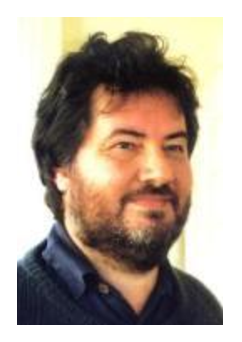
\includegraphics[height=5.5cm, width=4.5cm]{figuras/Ross.eps}\qquad
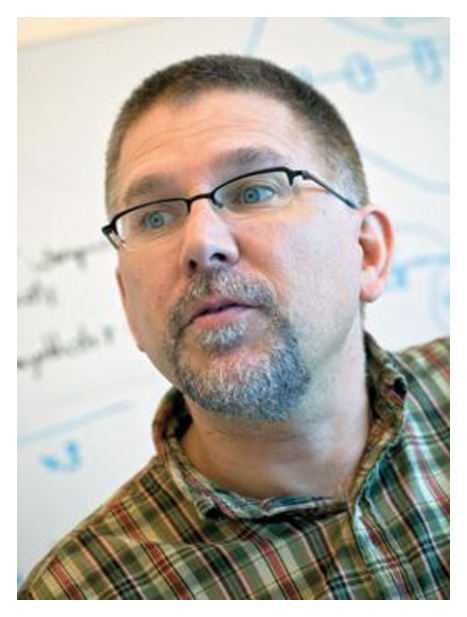
\includegraphics[height=5.5cm, width=4.5cm]{figuras/Robert.eps}
\caption{Ross Ihaka $\&$ Robert Gentleman}
\label{creadores}
\end{figure}

El desarrollo del lenguaje R como tal inició en el año de 1991, el progreso fue bastante bueno por lo que para Agosto de 1993 decidieron colocar algunas copias binarias del lenguaje R en Statlib\footnote{Sistema para la distribución de software estadístico vía electrónica.} y a su vez anunciaron al público el lanzamiento de la versión alfa del programa por medio de la lista de noticias de S (\emph{S news mailing list}). De manera sorpresiva un gran número de personas probaron el nuevo lenguaje y ofrecieron su retroalimentación sobre la versión que habían liberado, entre ellos el más persistente fue Martin Machler\footnote{Profesor de Estadística Computacional, Departamento de Matemática, Escuela Politécnica Federal de Zúrich.} que los animó a liberar el código fuente de manera que R se distribuya bajo licencia GNU General Public License, por lo cual en Junio de 1995 aparece la primera versión libre (\emph{open source}), el interés por el lenguaje R creció rapidamente al punto que para Marzo de 1996 fue necesario crear la propia lista de noticias y un año más tarde se tuvo que reemplazar por listas específicas: R-announce, R-help $\&$ R-devel, esto debido a la gran cantidad de consultas que realizaban los usuarios en varios temas relacionados.\newline

Para a mediados de 1997 se estableció el \texttt{R Core Group} o \texttt{R Core Team}, un grupo de desarrolladores talentosos y experimentados con permisos para administar el código fuente del lenguaje R, en sus inicios lo conformaban:
\begin{multicols}{3}
\begin{itemize}
   \item Ross Ihaka
   \item Robert Gentleman
   \item Martin Machler
   \item Doug Bates
   \item Peter Dalgaard
   \item Kurt Hornik
   \item Friedrich Leisch
   \item Thomas Lumley
   \item Paul Murrell
   \item Heiner Schwarte
   \item Luke Tierney
\end{itemize}
\end{multicols}

Entre sus tareas iniciales se encontraba realizar los cambios en el código fuente de acuerdo a los bugs reportados por los usuarios, todas las tareas se realizaban de manera voluntaria pues el grupo se formó sin fines de lucro, en la actualidad lo conforman alrededor de 20 personas que se encuentran en 11 diferentes cuidades del mundo.\newline

Se tuvo que esperar hasta el 29 de Febrero del 2000, para considerar que el software se encontraba completo y estable para liberar la versión 1.0.0. Desde entonces el programa se distribuye gratuitamente a través del repositorio \texttt{Comprehensive R Archive Network} (CRAN) en \url{http://www.r-project.org}, su mantenimiento se encuentra a cargo del grupo R Core Team desde el año 1997 asistido por una gran cantidad de colaboradores internacionales.\newline

El repositorio CRAN es fundamental para el uso del lenguaje R, pues en el sitio se almacena el ejecutable del programa así como las librerías que permiten ampliar sus capacidades. Con la finalidad de evitar el colapso del \emph{mundo estadístico} no se tiene una única ubicación al que todo mundo tiene acceso, el CRAN se \emph{refleja} en diferentes lugares de todo el mundo, de esta manera como residente de Ecuador podría acceder a una ubicación CRAN en Ecuador\footnote{En Ecuador se cuenta con el CRAN de la Escuela Politécnica del Litoral}, mientras que si se encuentra en un país que no tiene repositorio lo más recomendable es acceder a la copia del repositorio de un país cercano. Los países desarrollados como: EEUU, Alemania, Francia tienen múltiples CRAN's para abastecer a los usuarios. \emph{La filosofía básica es elegir un repositorio que se encuentre geográficamente cercano al usuario}.\newline 

R es considerado la versión libre del programa comercial S-Plus, el cual fue desarrollado para AT$\&$T Bell Laboratories por John M. Chambers y colaboradores en el año 1988, aunque son evidentes las diferencias entre R y S, la gran mayoría del código escrito para S funciona sin inconvenientes en R. En la actualidad el lenguaje S es distribuido por la empresa TIBCO bajo el nombre de S-PLUS.\newline

El mayor inconveniente para los nuevos usuarios de R es adaptarse a su interfaz gráfica que para muchos es \emph{poco amigable}, en el sentido que se deben tipear las funciones predefinidas o a su vez programar las funciones nuevas a diferencia de programas clásicos como SPSS, STATA, Minitab, etc., en los cuales se tienen botones o ventanas que despliegan opciones de análisis para el usuario. \newline

Dada la popularidad que ha adquirido el lenguaje en los últimos años se han desarrollado varias interfaces gráficas libres  GUIS's (Grafical User Interface) con el fin de volver más amigable la interacción con el usuario. Entre las interfaces más populares y utilizadas por la comunidad se encuentran:
\begin{multicols}{3}
\begin{itemize}
  \item RStudio
  \item Rattle
  \item Deducer
  \item RKWard
  \item Eclipse
  \item Knime
  \item R Analytic Flow
  \item JGR
  \item ESS
  \item Red -R
  \item R Commander
\end{itemize}
\end{multicols}

En el tercer capítulo del libro analizaremos con detalle las interfaces: RStudio y R Analityc Flow.

\section{Soporte}

El lenguaje R al ser un software libre carece de soporte técnico, sin embargo, debido a la gran cantidad de usuarios que ha adquirido en los últimos años han aparecido empresas que proveen varios tipos de soportes bajo pago. Entre las más destacadas se encuentran:
\begin{multicols}{2}
\begin{itemize}
  \item RStudio, Inc.
  \item Revolution Analytics, Inc.
  \item XL - Solutions Corporation.
  \item Quantide, Inc.
  \item R-Plus
  \item Statconn
\end{itemize}
\end{multicols}

De entre las empresas antes mencionadas se destaca de sobremanera Revolution Analytics\footnote{Revolution Analytics fue fundada en el año 2007 con la finalidad de dar soporte comercial al software Revolution R, adicionalmente provee componentes tales como: ParallelR, RevoScaleR, RevoDeployR, etc.}, Inc. por haber optimizado el código fuente del lenguaje R lo cual ha permitido que el programa sea multicore, es decir, a través de estas modificaciones se logró aprovechar al máximo la funcionalidad de todos los núcleos de los procesadores (16 núcleos para procesadores Core i7, etc.). El impacto inmediato del multicore se ve reflejado en la mayor velocidad de procesamiento de información permitiendo de este modo trabajar con grandes cantidades de datos sin ningún problema, así como también en la reducción del tiempo de ejecución.

\begin{figure}[H]
\centering
\includegraphics[scale=.6]{figuras/logo_rro.eps}
\caption{Revolution R Open}
\end{figure}

El programa optimizado es $100\%$ compatible con el software relacionado a R (paquetes, interfaces, etc.) y puede obtenerse desde el sitio web \url{http://www.revolutionanalytics.com} como \texttt{Revolution R Open} de forma gratuita bajo licencia GPL, sin embargo en el caso de requerir soporte se puede adquirir la versión pagada \texttt{Revolution R Enterprise}.


\section{Funcionamiento}

El programa R es un lenguaje orientado a objetos (OOP\footnote{La programación OOP está basada en varias técnicas: herencia, clasificación, identidad, polimorfismo y encapsulamiento.}) dise\~nado en un entorno auténtico bajo el cual esconde su simplicidad y flexibilidad, lo cual permite a sus usuarios a\~nadir funcionalidad mediante la definición de nuevas \emph{funciones}. El término \emph{orientado a objetos} hace referencia a un paradigma de la programación que emplea objetos en sus interacciones y diseño de aplicaciones. R almacena sus variables, datos, funciones, resultados, etc., en la memoria activa del computador en forma de objetos con un nombre específico y pueden ser modificados o manipulados por el usuario mediante operadores y funciones.\newline

El hecho que R sea un lenguaje de programación puede desmotivar a muchos usuarios, los cuales piensan que para iniciarse en el programa se necesita \emph{alma de programador} lo cual no es cierto. Primero R es un lenguaje interpretado similar a Java, y segundo no es un lenguaje compilado a diferencia de C, C++, Fortran, Pascal, ect. sino más bien mediante comandos ingresados por teclado los cuales se ejecutan directamente sin necesidad de construir archivos ejecutables. En su mayoría R se encuentra programado en C++, Python y Fortran, esto implica que R tiene la capacidad de interpretar código externo mediante el uso de ciertas librerías. La utilidad básica de lo anterior se encuentra en elaborar scripts, por ejemplo en C++, que emplean menor tiempo de ejecución.\newline 

El programa R incluye 8 bibliotecas o paquetes estándar, sin embargo, las capacidades de R pueden ser ampliadas fácilmente mediante la incorporación de paquetes que se encuentran disponibles en varios repositorios como:
\begin{multicols}{2}
\begin{itemize}
  \item CRAN
  \item BioConductor
  \item Github
  \item Omegahat
  \item MRAN
  \item RForge, entre otros.
\end{itemize}
\end{multicols}

Los paquetes estándar pueden ser visualizados a través del comando:
\begin{knitrout}
\definecolor{shadecolor}{rgb}{0.969, 0.969, 0.969}\color{fgcolor}\begin{kframe}
\begin{alltt}
\hlkwd{search}\hlstd{()}
\end{alltt}
\begin{verbatim}
##  [1] ".GlobalEnv"         "package:data.table" "package:dplyr"     
##  [4] "package:knitr"      "package:stats"      "package:graphics"  
##  [7] "package:grDevices"  "package:utils"      "package:datasets"  
## [10] "package:methods"    "Autoloads"          "package:base"
\end{verbatim}
\end{kframe}
\end{knitrout}

En la actualidad\footnote{Información obtenida al 21 de Septiembre 2015.} existen 7190 paquetes válidos en el repositorio CRAN, que se encuentran ordenados por fecha de publicación o alfabéticamente agrupadas en diversas líneas de investigación.

\section{Ventajas}

Entre las principales ventajas que posee el software R podemos anotar lo siguiente:
\begin{itemize}
  \item Al tratarse de un software libre el costo es nulo.
  \item Se han implementado una gran cantidad de métodos estadísticos desde los más básicos hasta los más avanzados y modernos. Todos los métodos se encuentran organizados en librerías, que se encuentran en constante crecimiento.
  \item Capacidad para acceder a datos de múltiples formatos. En la actualidad existen varias librerías para leer datos desde SPSS, SAS, STATA, MySQL, Excel, etc.
  \item Gran capacidad para la manipulación de datos y funciones, así como para la generación de gráficos de alta calidad.
  \item Facilidad para enlazarse con LaTeX y generar reportes dinámicos.
  \item Amplia bibliografía tanto en internet como en libros publicados por prestigiosas editoriales como: Springer, Wiley, O'Reilly, Chapman $\&$ Hall/CRC, etc.
  \item Fácil visualización e interpretación de los algoritmos implementados en R con lo cual el usuario puede conocer exactamente lo que el ordenador ejecuta.
  \item Permite visualizar los algoritmos en él implementados, modificarlos y ajustarlos a nuestras necesidades (esto no es permitido en los softwares licenciados).
  \item Una gran comunidad de usuarios, lo cual permite obtener ayuda de manera fácil de expertos por medio de la R help mailing list, entre otros.
\end{itemize}

\section{Desventajas}

Los inconvenientes a los cuales se deben enfrentar los usuarios de R son:
\begin{itemize}
  \item Al ser un programa libre carece de un departamento de atención al cliente al cual se pueda recurrir en caso de que se reporte un inconveniente con el mismo. Sin embargo, existe una comunidad en crecimiento de usuarios de R que se encuentran dispuestos a colaborar desinteresadamente en la resolución de problemas.
  \item El software R como tal no dispone de una interfaz amigable para el usuario, las tareas se llevan a cabo a través de líneas de comando lo cual puede resultar difícil para el usuario común. No obstante con el desarrollo de GUI's se ha facilitado en gran medida la experiencia del programa con el usuario común.
  \item El código en R es interpretado, no compilado, lo cual puede ocasionar una ejecución lenta en ocasiones en las que se realizan simulaciones intensas. Con el fin de remediar lo anterior el grupo R Core Team a partir de la versión 2.14 ha precompilado todas las funciones y librerías de R con el objetivo de acelerar la ejecución.
  \item R no es particularmente un lenguaje de programación rápido, si a eso sumamos que muchos usuarios escriben pobremente su código, obtenemos como resultado un funcionamiento lento.
\end{itemize}

\section{Usuarios en el mundo}

Han transcurrido 22 años desde el aparecimiento de R y el número de usuarios sigue creciendo día a día\footnote{Se estima que existe alrededor de dos milones de usuarios en todo el mundo.}. Lo que comenzó como un proyecto para proporcionar un \emph{software estadístico}, hoy en día se ha convertido en una solución estándar para el análisis de datos en todo el mundo.

\begin{figure}[H]
\centering
\includegraphics[scale=.5]{figuras/rapporter.pdf}
\caption{Actividad de los usuarios}
\end{figure}

Los países con mayor cantidad de usuarios activos son:
\begin{multicols}{2}
\begin{enumerate}
   \item Suiza
   \item Nueva Zelanda
   \item Austria
   \item Irlanda
   \item Estados Unidos
   \item Australia
   \item Singapur
   \item Dinamarca
   \item Reino Unido
   \item Canadá
\end{enumerate}
\end{multicols}

Llama la atención que cada vez más se incrementa el número de cursos y cantidad de libros relacionados con el programa R. Además los usuarios optan por escribir en sus blogs muchas de sus experiencias con ciertos paquetes lo cual se ha convertido en material de gran ayuda para los principiantes.

\subsection{UseR!}

Con la finalidad de conocer a otros usuarios, aprender de los expertos, compartir experiencias y participar de tutoriales se ha venido llevando a cabo conferencias internacionales anualmente desde el 2004.

\begin{figure}[H]
\centering
\includegraphics[scale=.6]{figuras/useR.pdf}
\caption{Logo UseR!}
\end{figure}

La última conferencia \texttt{UseR!} se llevó a cabo entre el 30 de Junio y 3 de Julio de 2015 en la ciudad de Aalborg, Dinamarca y contó con más de $660$ participantes de $40$ diferentes países. Mientras que para el año 2016, la conferencia tendrá lugar en la Universidad de Stanford (California, EEUU) entre el 27 y 30 de Junio.\newline

Para mayor información: \url{https://www.r-project.org/conferences.html}

\subsection{R User Groups}

Debido que la comunidad de usuarios a nivel mundial es demasiado grande, existen grupos más pequeños formados por: temas especificos, idioma, ubicación, etc., que permiten interactuar de manera sencilla con otros usuarios. Actualmente, existen alrededor de $150$ grupos registrados en el directorio de Revolution Analytics, la gran mayoría de ellos se reúnen periodicamente y cuentan con una página web en Meetup que les permite compartir noticias y detalles de próximas reuniones.




\chapter{Instalación y actualización}

En esta sección mostraremos los pasos a seguir para la instalación, actualización del programa y sus paquetes. Asumiremos que el usuario se encuentra trabajando sobre un computador con sistema Windows o Mac, sin embargo, no existe mayor diferencia en los pasos a seguir en el caso que el usuario use un sistema operativo o plataforma diferente.

\section{Instalación de R}

La descarga del programa R se describe en los siguientes pasos:
\begin{enumerate}
  \item Accedemos al sitio web del R Project a través de un navegador tecleando la dirección: \url{http://www.r-project.org}.
  \begin{figure}[H]
    \centering
    \includegraphics[scale=.45]{figuras/install1.eps}
    \caption{Página web R-Project}
    \label{rproject}
  \end{figure}
  
  \item Nos dirigimos al enlace de la CRAN ubicado en la parte superior izquierda y elegimos un repositorio cercano a nuestra localidad. En nuestro caso seleccionamos el repositorio de la Escuela Politécnica de Litoral.
  \begin{figure}[H]
    \centering
    
\includegraphics[width=4cm,height=1.2cm]{figuras/install2.eps}
    \caption{Repositorio Espol}
    \label{respol}
  \end{figure}
  
  \item En la parte superior de la página nos dirigimos al enlace \texttt{Download and install R}, seguido elegimos el sistema operativo.
  \begin{figure}[H]
    \centering
    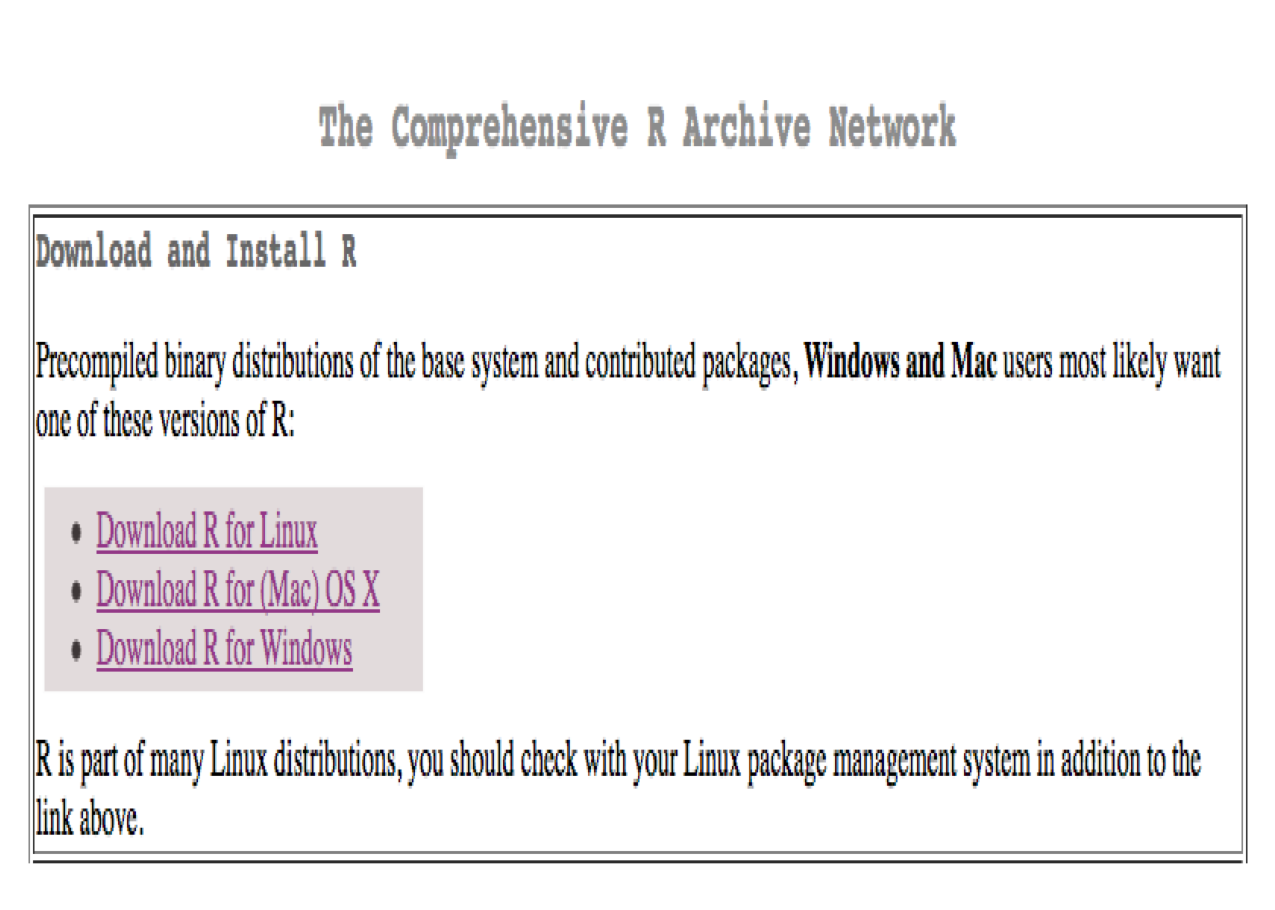
\includegraphics[width=10.5cm,height=3.7cm]{figuras/install3.eps}
    \caption{Selección Sistema Operativo}
    \label{soperativo}
  \end{figure}
  
  \item Elegimos el subdirectorio \texttt{base}.
  \begin{figure}[H]
    \centering
    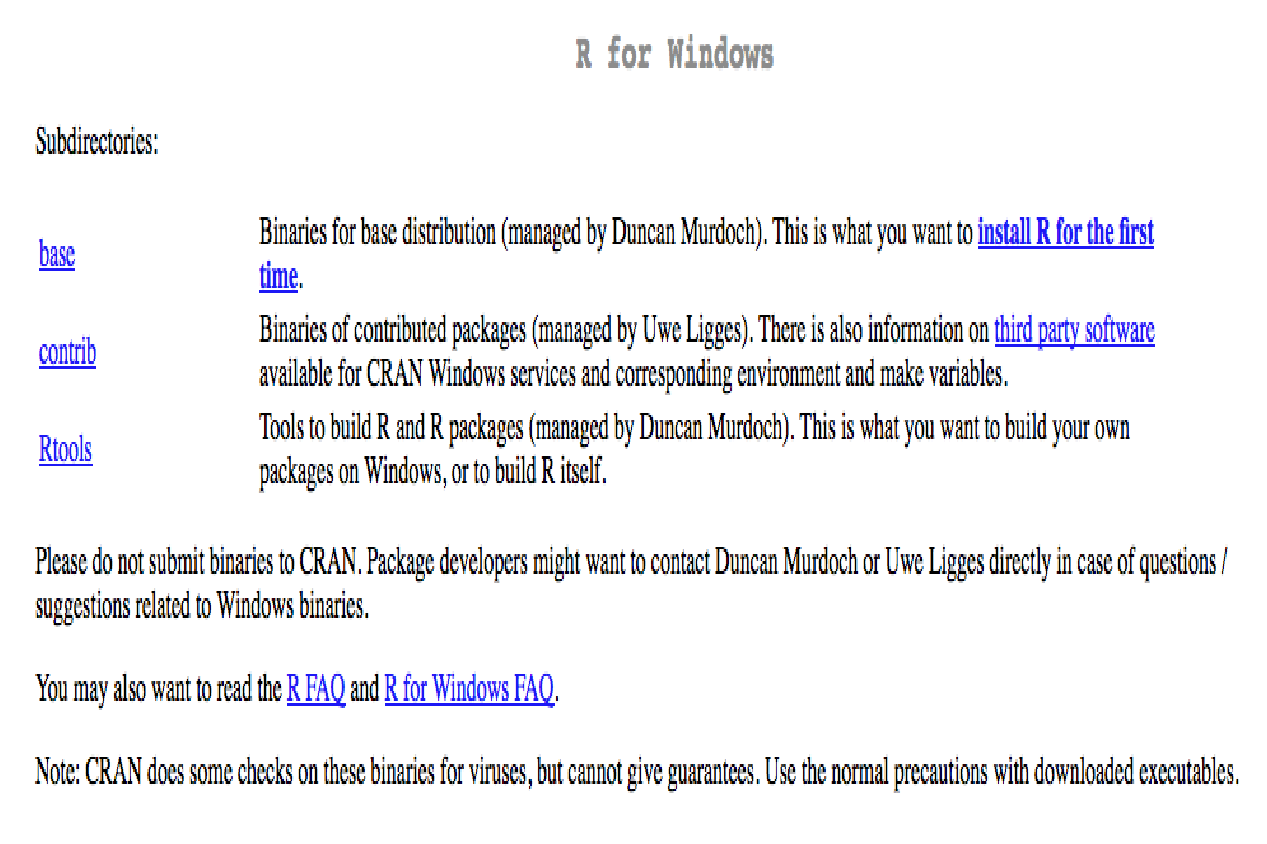
\includegraphics[width=11.5cm,height=4.2cm]{figuras/install4.eps}
    \caption{Subdirectorios}
    \label{subdirectorio}
  \end{figure}
  
  \item Finalmente, damos click sobre \texttt{Download R X.Y.Z for Windows}, con lo cual descargamos la versión de R más reciente.
  \begin{figure}[H]
    \centering
    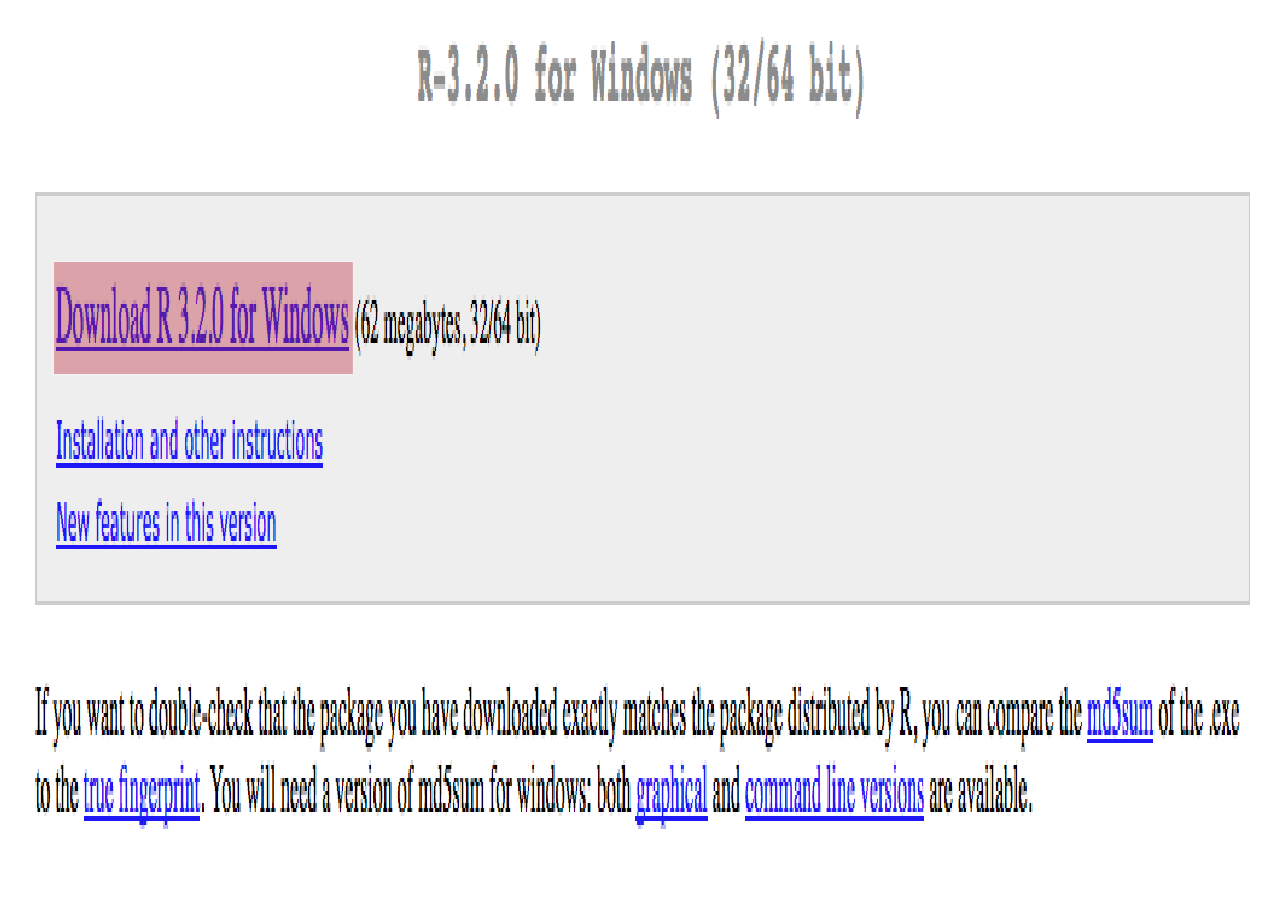
\includegraphics[width=11.5cm,height=3.2cm]{figuras/install5.eps}
    \caption{Descarga programa}
    \label{download}
  \end{figure}
\end{enumerate}

Una vez obtenido el ejecutable del programa procedemos con la instalación:
\begin{enumerate}
   \item Damos doble click sobre el ejecutable y seleccionamos el idioma que nos guiará en el proceso de instalación.
   \begin{figure}[H]
    \centering
    \includegraphics[scale=0.6]{figuras/r01.pdf}
    \caption{Seleccionamos \texttt{Español} como idioma}
  \end{figure}
   \item En las siguientes dos ventanas damos click sobre el botón \emph{Siguiente}. En caso de requerirlo ponemos revisar los términos establecidos para el uso del software.
   \begin{figure}[H]
    \centering
    \includegraphics[scale=0.54]{figuras/r02.pdf}\qquad
    \includegraphics[scale=0.54]{figuras/r03.pdf}
    \caption{Click en \texttt{Siguiente}}
  \end{figure}
   \item Seleccionamos el lugar en disco para albergar los archivos del programa o simplemente aceptamos la dirección por defecto (recomendado).
   \begin{figure}[H]
    \centering
    \includegraphics[scale=0.54]{figuras/r04.pdf}
    \caption{Seleccionamos el directorio de instalación}
  \end{figure}
   \item Seleccionamos los componentes del programa ha ser instalados, por defecto se instalan todos los componentes, sin embargo no es necesario (se podría instalar únicamente los dos primeros componentes).
   \begin{figure}[H]
    \centering
    \includegraphics[scale=0.54]{figuras/r05.pdf}
    \caption{Componentes del programa}
  \end{figure}
   \item Para las tres siguientes ventanas simplemente damos click en el botón \emph{Siguiente} de acuerdo a la configuración mostrada a continuación:
   \begin{figure}[H]
    \centering
    \includegraphics[scale=0.54]{figuras/r06.pdf}\qquad
    \includegraphics[scale=0.54]{figuras/r07.pdf}\qquad
    \includegraphics[scale=0.54]{figuras/r08.pdf}
    \caption{Click en \texttt{Siguiente}}
  \end{figure}
   \item Para la configuración del \emph{proxi} debemos tomar en consideración si la red de internet con la cual trabajamos tiene seguridades o no. En caso afirmativo seleccionaremos \emph{Internet2} (recomendado), caso contrario \emph{Standard}.
   \begin{figure}[H]
    \centering
    \includegraphics[scale=0.54]{figuras/r09.pdf}
    \caption{Configuración Proxi}
  \end{figure}
   \item En las últimas dos ventanas damos click sobre el botón \emph{Siguiente} de acuerdo a la configuración mostrada a continuación:
   \begin{figure}[H]
    \centering
    \includegraphics[scale=0.54]{figuras/r10.pdf}\qquad
    \includegraphics[scale=0.54]{figuras/r11.pdf}
    \caption{Click en \texttt{Siguiente}}
  \end{figure}
\end{enumerate}

Con los pasos antes descritos lograremos tener el programa $100\%$ funcional y listo para utilizarlo en nuestro computador.\newline

En la actualidad, el software R puede ser instalado incluso sobre la plataforma Android\footnote{\url{https://play.google.com/store/apps/details?id=com.appsopensource.R&hl=es_419}}, esto permite que muchos usuarios puedan tener acceso al programa en todo momento con tan sólo contar con un smartphone operativo.

\section{Entorno de trabajo}

Es de gran importancia para el usuario de R conocer el entorno de trabajo, y es precisamente lo que trataremos en esta sección. Iniciaremos explicando  la barra de herramientas, la misma que consta de las secciones: Archivo, Editar, Visualizar, Misc, Paquetes, Ventanas y Ayuda.

\begin{figure}[H]
\centering
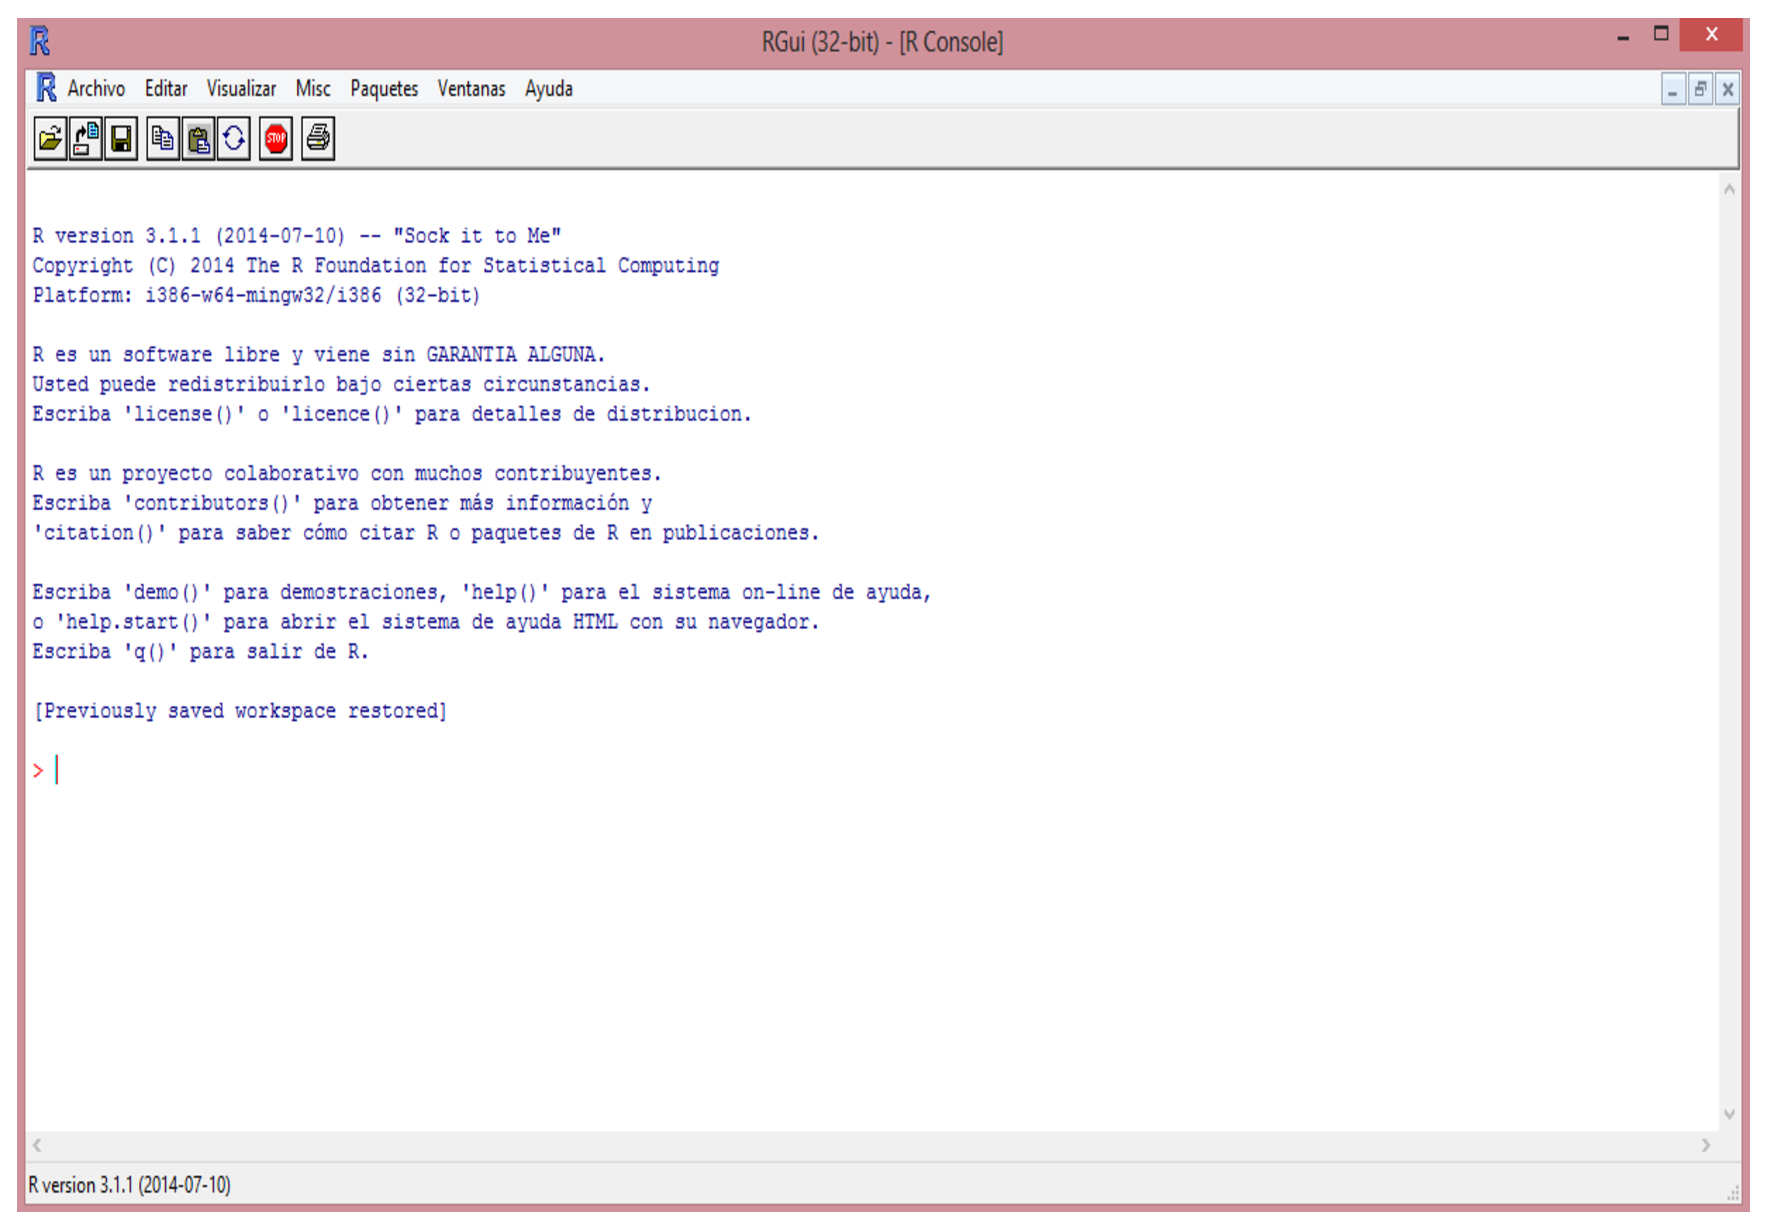
\includegraphics[scale=.4]{figuras/console.eps}
\caption{Entorno de trabajo de R}
\label{entorno}
\end{figure}


%\begin{itemize}
\subsection{Archivo}

En esta sección se podrá tratar todo lo relacionado con el área de trabajo, manejo de archivos y salida del programa. Los elementos que lo componen son:
  \begin{figure}[H]
  \centering
  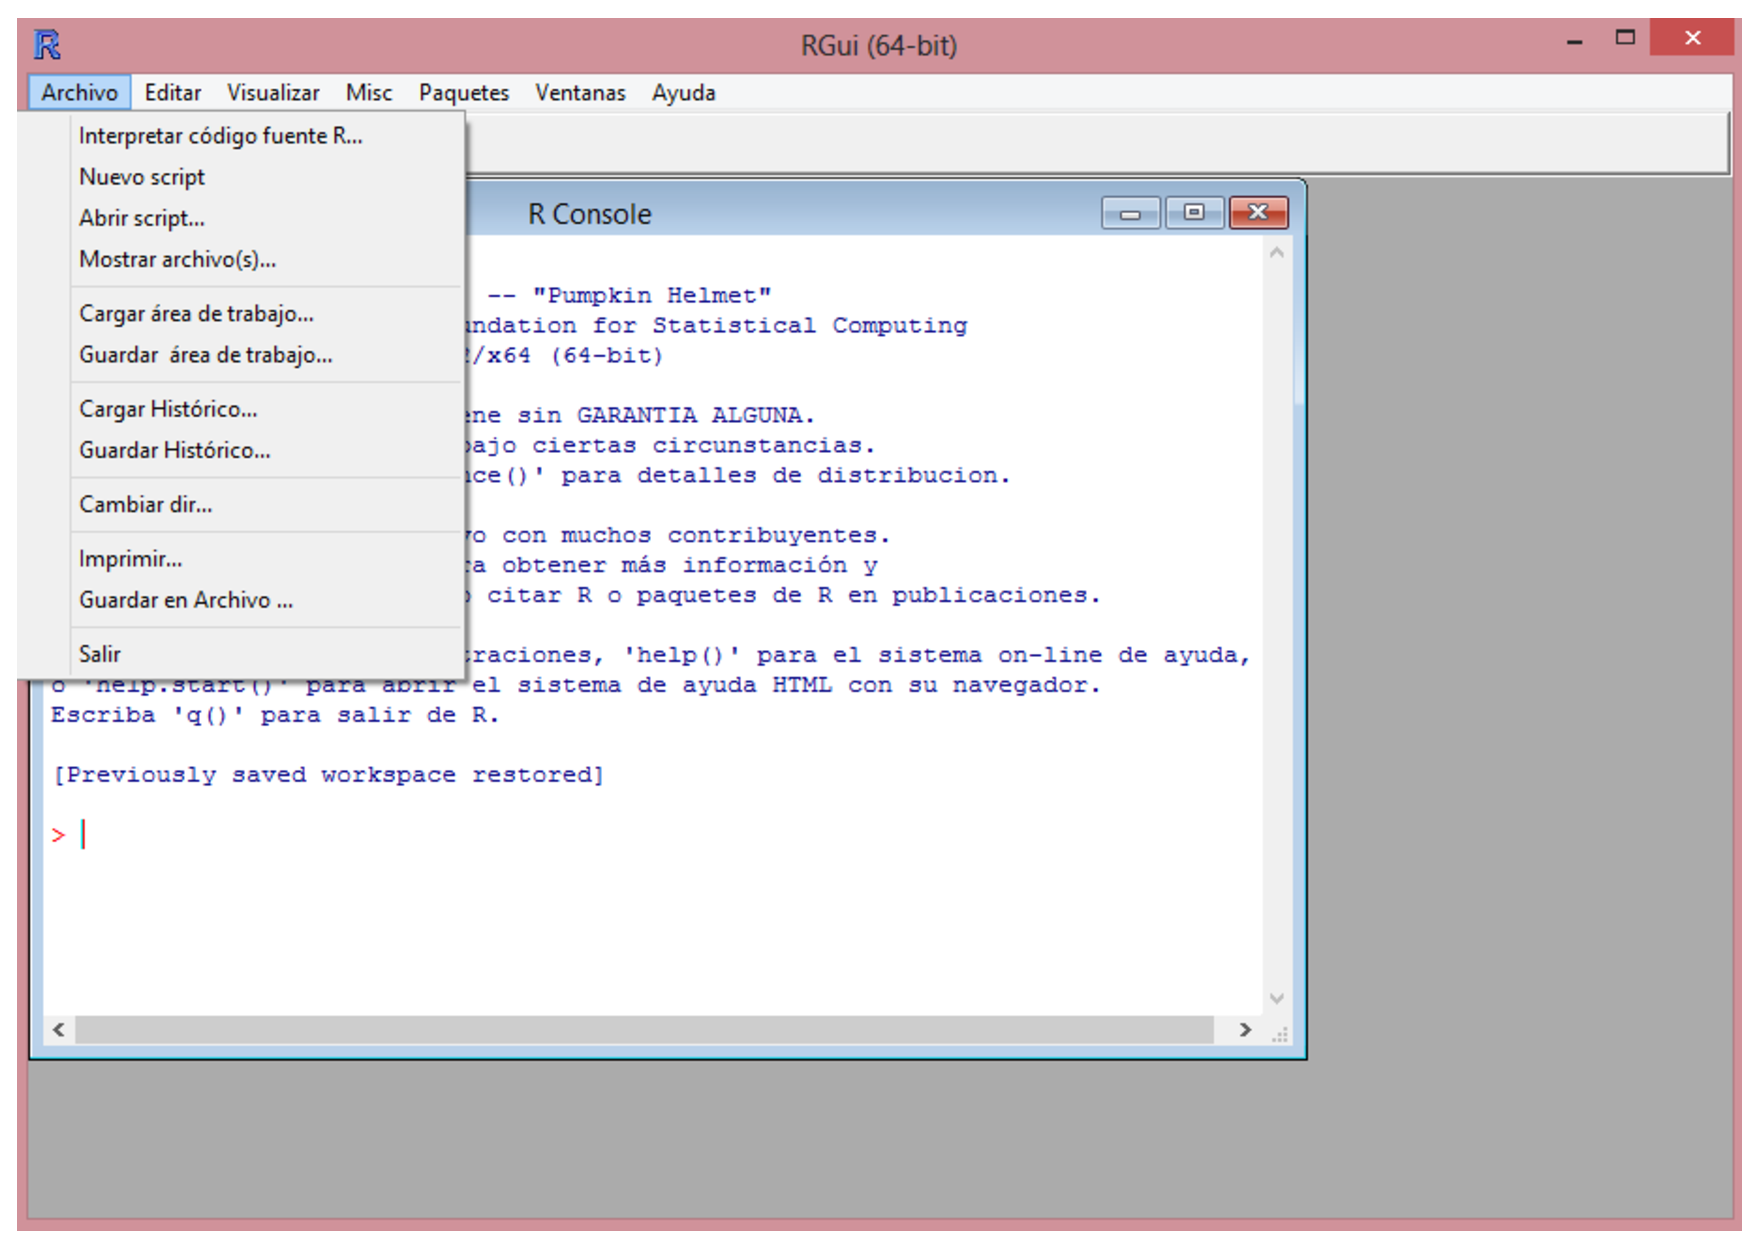
\includegraphics[scale=.4]{figuras/archivo.eps}
  \caption{Sección Archivo}
  \label{archivo}
  \end{figure}

\begin{itemize}
      \item {\bf Interpretar código fuente R:} Hay que recordar que R es un lenguaje de programación derivado del S, es por ello que podemos realizar programas en un editor externo, con esta opción podemos ejecutar dicho programa en la consola siempre y cuando, la extensión de guardado sea del tipo .R.
      \item {\bf Nuevo script:} Si lo ejecutamos, se nos abrirá un editor de lenguaje R para crear script que luegos podemos llamar desde la consola, el tipo de archivo que podemos generar son R o S.
      \item {\bf Abrir script:} Los script que hemos generados o que tengamos del tipo R o S podemos abrirlos en un editor para poder editarlos.
      \item {\bf Mostrar archivo(s):} Siver para abrir y poder visualizar o editar cualquier archivo, es interesante para los que tengan relación con el lenguaje R o S. Se diferencia con la opción Abrir script de que éste no puede editarlos directamente, simplemente visualizarlos. Se pueden abrir varios archivos a la vez.
      \item {\bf Cargar área de trabajo:} Pues como su nombre indica, sirve para cargar un área de trabajo que hayamos configurado y guardado previamente, es útil por ejemplo, cuando hemos definido el tipo de letra, el espacio de trabajo, los colores, etc, y queremos usarlo. La extensión común es .RData aunque también puede cargarse entornos de trabajo con formato antiguo tipo .rda.
      \item {\bf Guardar área de trabajo:} Cuando se haya configurado el entorno de consola de R, colores, tipo de letra, tamaño, etc, podemos guardarlo para cargarlo posteriormente en futuras aplicaciones ya que el propio programa R no guarda, de momento, dicha configuración. El formato del entorno de trabajo es .RData.
      \item {\bf Cargar Histórico:} Podemos cargar el archivo de comandos que se hayan ejecutado en una sesión previamente guardada. El formato de salida es .history.
      \item {\bf Guardar Histórico:} Con él, podemos guardar los comandos que hayamos instroducido por consola en una sesión. El formato de guardado es .history.
      \item {\bf Cambiar dir:} Podemos configurar el directorio de trabajo que está definido por defecto cuando se instaló el programa.
      \item {\bf Imprimir:} Podemos configurar e imprimir el entorno de trabajo de R, la consola.
      \item {\bf Guardar en archivo:} Se guardará todo lo que se haya escrito por la consola en formato .txt que después podremos recuperar.
      \item {\bf Salir:} Sirve para salir del programa R, antes nos preguntará si queremos guardar el área de trabajo.
\end{itemize}

\subsection{Editar}

Es la sección encargada de la edición de datos y de la configuración del entorno de trabajo.
  \begin{itemize}
  \begin{figure}[H]
  \centering
  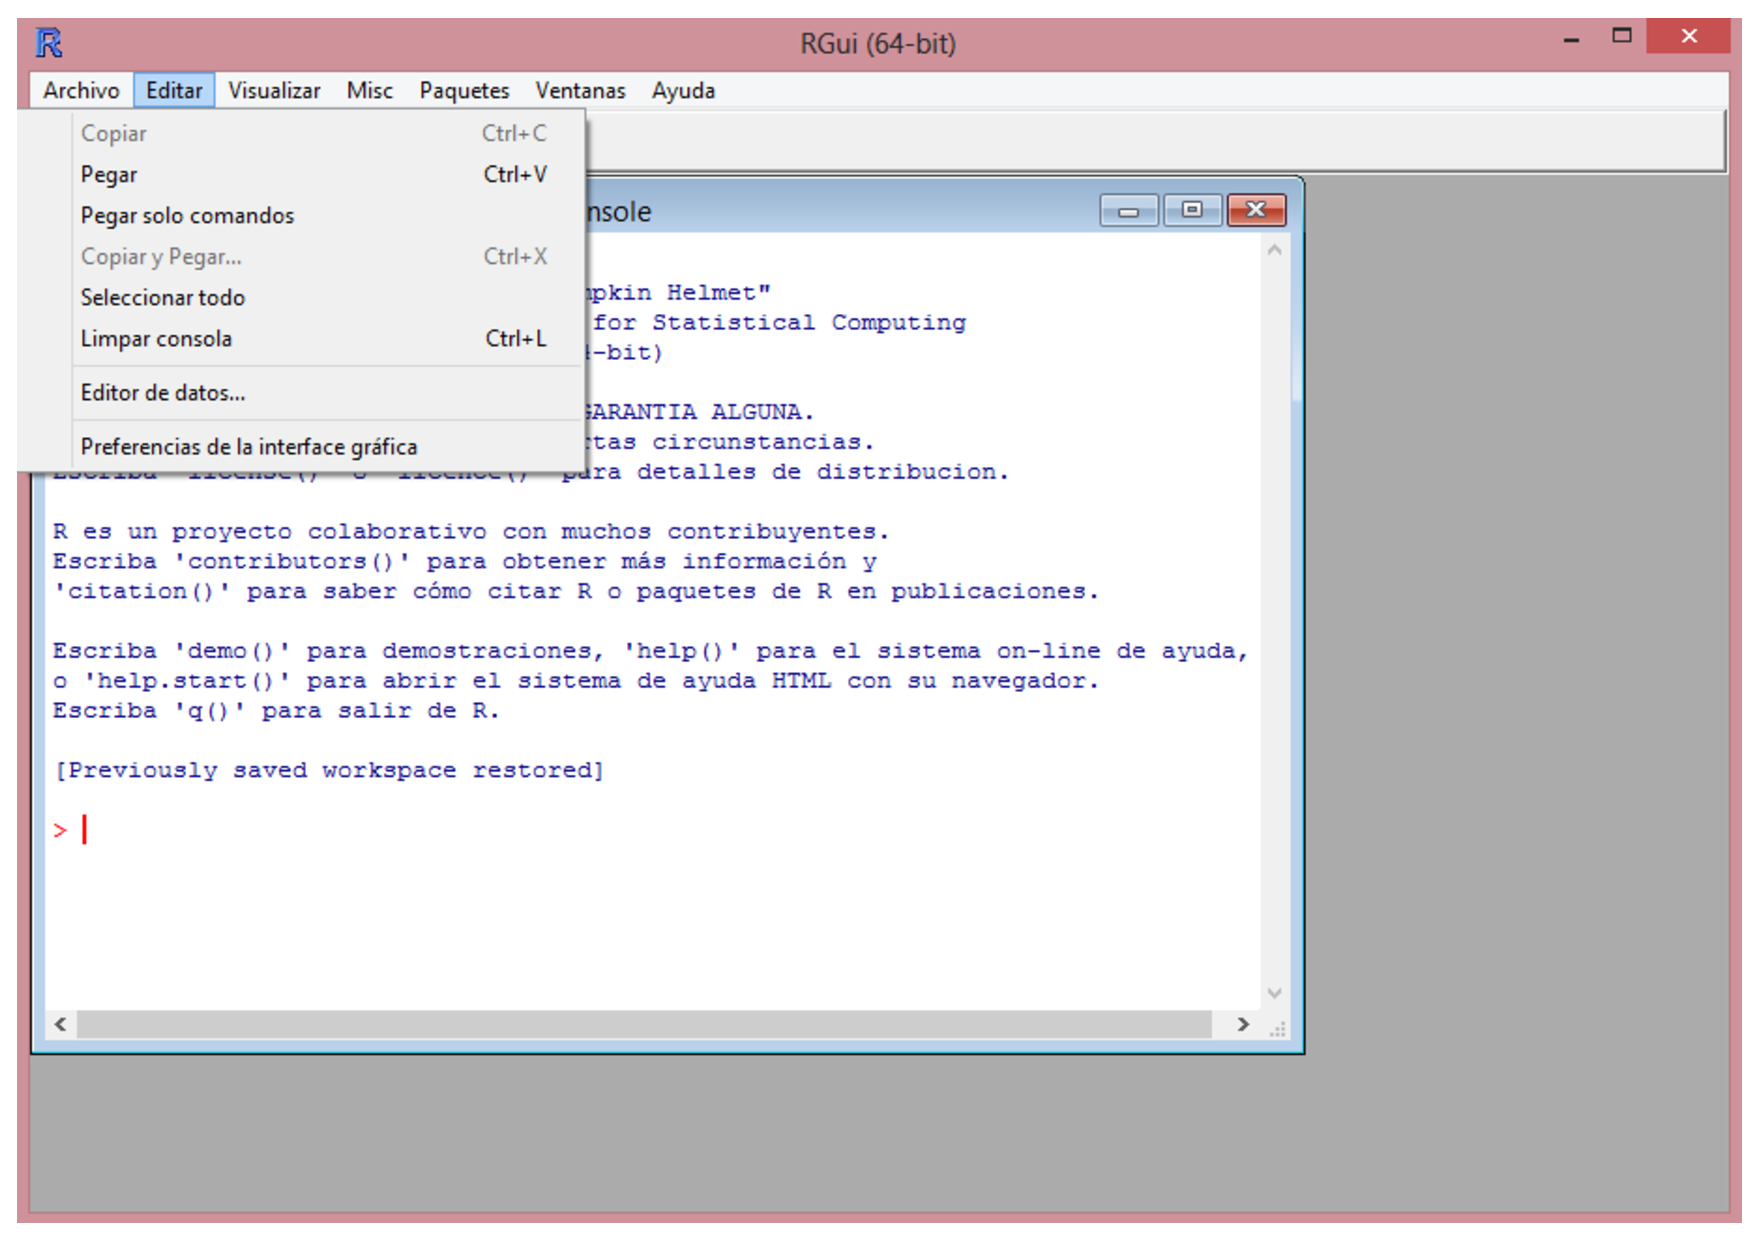
\includegraphics[scale=.4]{figuras/editar.eps}
  \caption{Sección Editar}
  \label{editar}
  \end{figure}

\begin{itemize}
      \item {\bf Copiar:}Podemos copiar al portapapeles el comando o sentencia o lo que queramos de la consola. Para acceder de forma
      rápida por teclado se debe pulsar: Ctrl + C.
      \item {\bf Pegar:} Podemos pegar en la consola aquello que tengamos en el portapapeles. Para acceder de forma rápida por teclado
      se debe pulsar: Ctrl + V.
      \item {\bf Pegar solo comandos:} La diferencia básica con la opción Pegar es que con esta opción, sólo se pegarán en la consola
      aquello que sea comandos para ejecutarse.
      \item {\bf Copiar y Pegar:} Todo aquello que copiemos, directamente se pegará, de forma inmediata, en la consola. Para acceder de
      forma rápida por teclado se debe pulsar: Ctrl + X.
      \item {\bf Seleccionar todo:} Como su nombre indica, se selecciona todo lo que esté presente en la consola.
      \item {\bf Limpiar consola:} Se borrarán todo lo que esté presente en la consola, pero ojo, no se borrarán las variables y estructuras definidas. Es útil cuando tenemos en la consola mucha información que ya no es útil. Para acceder de forma rápida por
      teclado se debe pulsar: Ctrl + L.
      \item {\bf Editor de datos:} Podemos definir datos (vectores, estructuras, funciones, etc) y guardarlos para posteriormente llamarlos en la consola. Estos datos estarán definidos en la consola cuando se guarde.
      \item {\bf Preferencias de la interfaz gráfica:} En esta opción es donde podremos configurar todo lo relacionado a la visualización de texto reflejado en la consola: tamaño de letra, colores, tipo de letra, etc. También, se puede configurar el entorno de trabajo, para multiventana o una única ventana.
\end{itemize}

\subsection{Visualizar} 

Activa la visualización de algunos iconos en la parte superior tales como: Abrir script, Cargar área de trabajo, etc., mismas que ya se detallaron anteriormente.

  \begin{figure}[H]
  \centering
  \includegraphics[scale=.4]{figuras/visualizar.eps}
  \caption{Sección Visualizar}
  \label{visualizar}
  \end{figure}

\subsection{Misc} 

Esta es la sección denominada misceláneas, donde hay más de un control interesante.

  \begin{figure}[H]
  \centering
  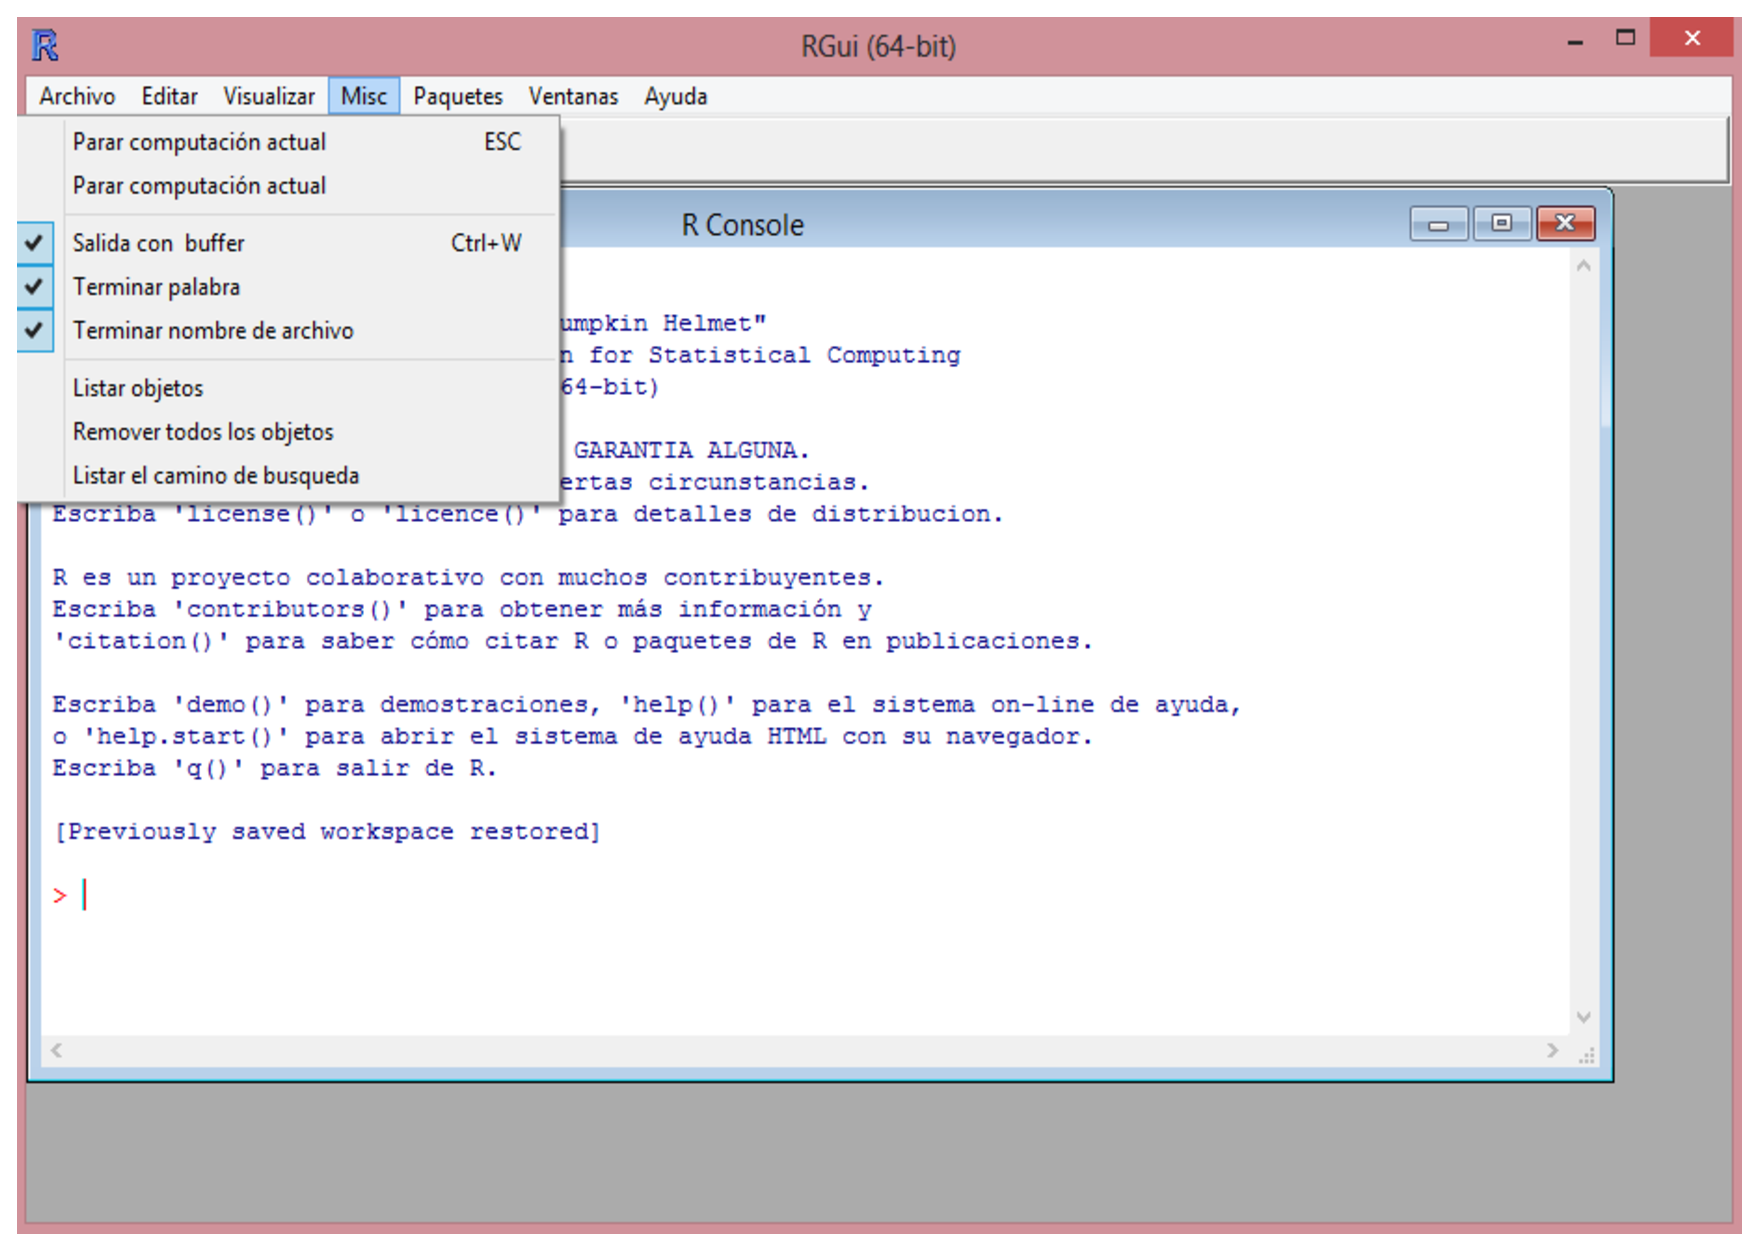
\includegraphics[scale=.4]{figuras/misc.eps}
  \caption{Sección Misc}
  \label{misc}
  \end{figure}

\begin{itemize}
      \item {\bf Parar computación actual:} Este control es muy interesante y útil, con él, podremos parar cualquier archivo, sentencia o código que esté ejecutando la consola R. Para acceder de forma rápida por teclado se debe pulsar: ESC.
      \item {\bf Salida con buffer:} Para acceder de forma rápida por teclado se debe pulsar: Ctrl + W.
      \item {\bf Terminar palabra:} Es una ayuda interactiva, que nos ayuda a completar las palabras mientras estamos escribiendo en caso que la consola las reconozca.
      \item {\bf Terminar nombre de archivo:} Realiza la misma función que la opción Terminar palabra pero en archivos.
      \item {\bf Listar objetos:} Se nos mostrará por consola los objetos que hasta en este momento hemos definido en la consola.
      \item {\bf Remover todos los objetos:} Como su nombre indica, elimina de memoria todos los objetos que hayamos definido (datos, variables, matrices, vectores, etc) en la consola de R. Cuando pulsemos sobre dicha opción, el programa, nos preguntará si realmente queremos borrarlos.
      \item {\bf Listar el camino de búsqueda:} Nos ofrece por consola las librerias y complementos que tenemos instalados en R.
\end{itemize}

\subsection{Paquetes} 

Dedicado al manejo de las librerías que posee el programa R.
  \begin{figure}[H]
  \centering
  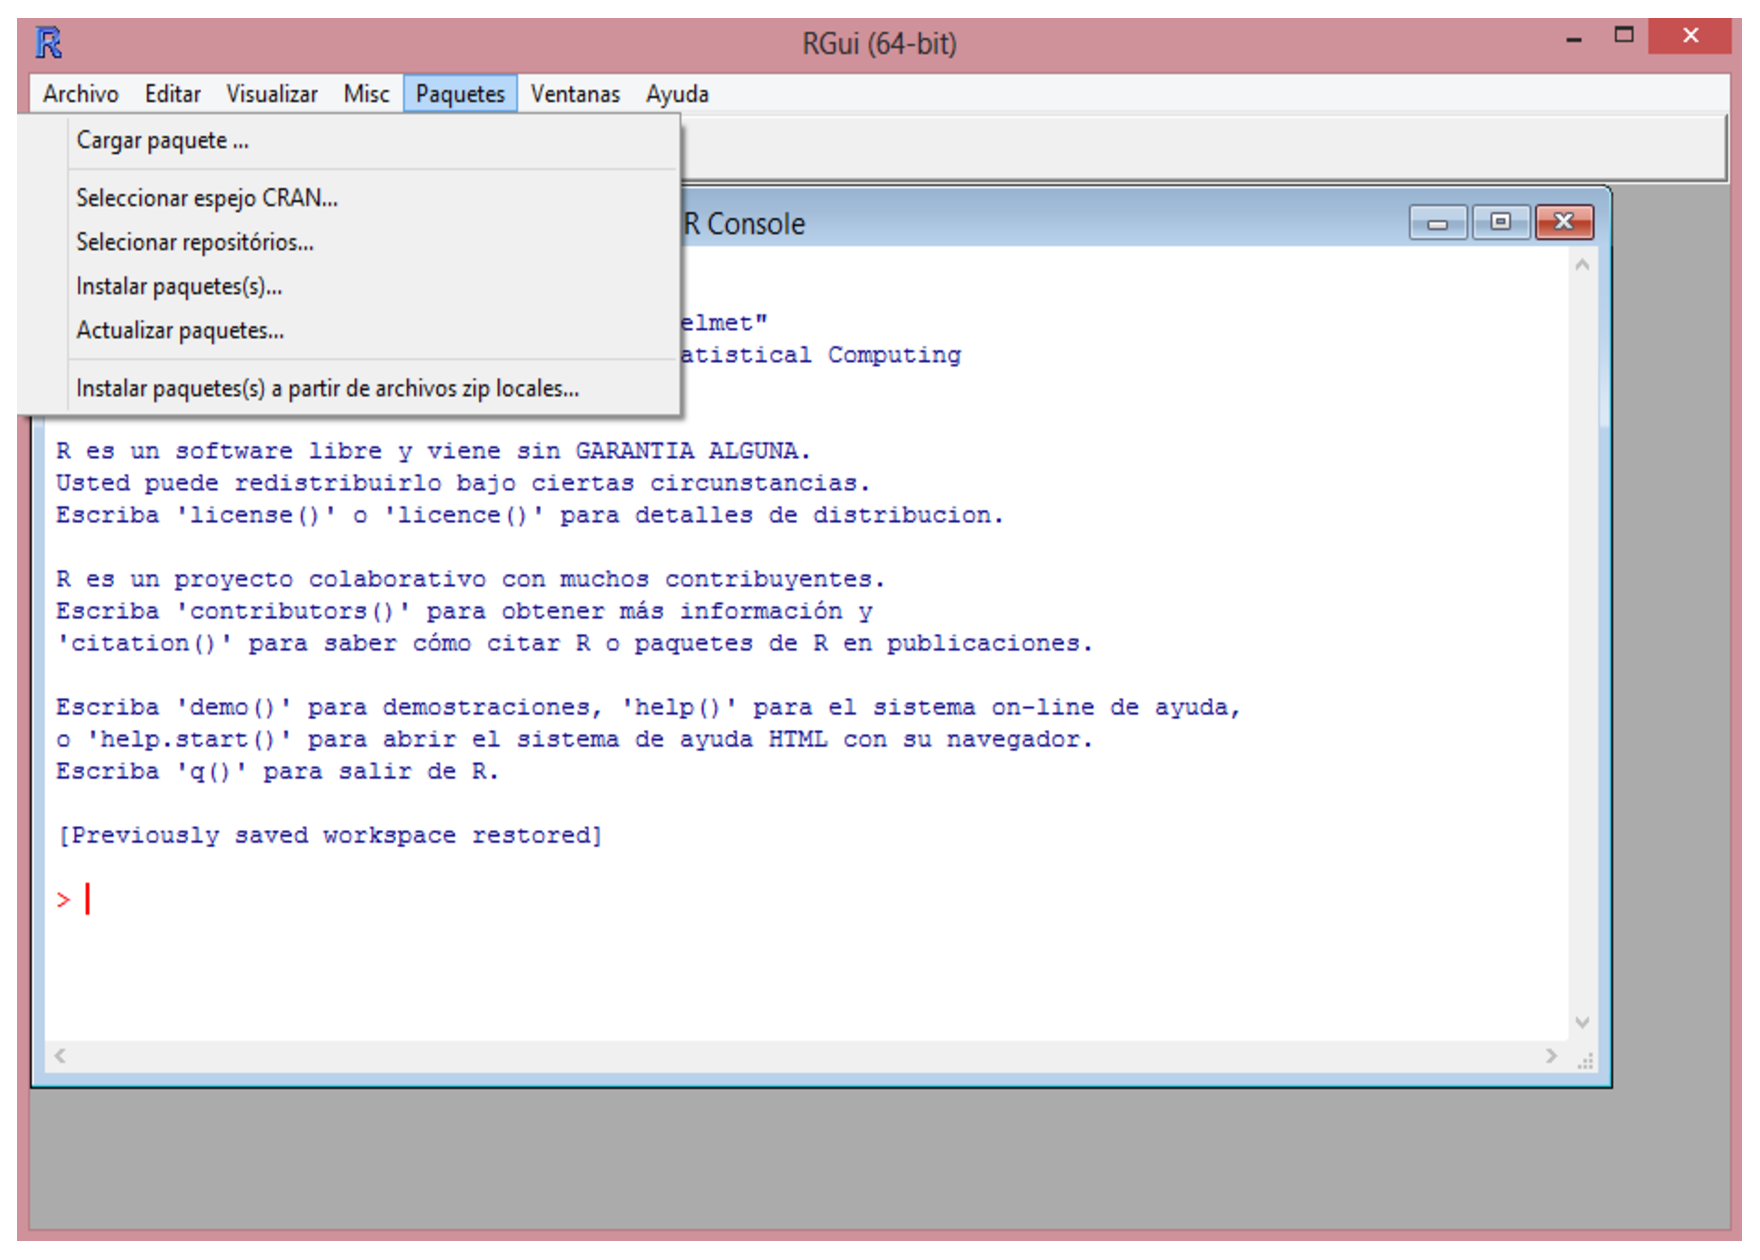
\includegraphics[scale=.4]{figuras/paquetes.eps}
  \caption{Sección Paquetes}
  \label{paquetes}
  \end{figure}

\begin{itemize}
      \item {\bf Cargar paquete:} Con él, podemos cargar en la consola cualquier librería que tengamos instalada.
      \item {\bf Seleccionar espejo CRAN:} Sirve para configurar el servidor de librerías.
      \item {\bf Seleccionar repositórios:} En consola nos mostrará los repositorios que tenemos instalados y nos pedirá cual usar para la sesión activa.
      \item {\bf Instalar paquetes(s):} Podremos actualizar o instalar librerías nuevas en red, para ello, debemos elegir un servidor.
      \item {\bf Actualizar paquetes(s):} Podemos actualizar las librerías que tengamos instaladas en caso de haber una actualización reciente por red, para ello, debemos seleccionar un servidor
      \item {\bf Instalar paquetes(s) a partir de archivos zip locales:} En caso de haber descargado una librería y tenerla en nuestro ordenador, podemos instalarlo mediante esta opción.
\end{itemize}

\subsection{Ventanas} 

Permite configurar la visualización de las ventanas: consola, área de gráficos y editor de script en modo vertical, horizontal, etc.

  \begin{figure}[H]
  \centering
  \includegraphics[scale=.4]{figuras/ventanas.eps}
  \caption{Sección Ventanas}
  \label{ventanas}
  \end{figure}

\subsection{Ayuda} 
  
Es un apartado que debemos tenerlo siempre presente, ya que en él se dispone al usuario, los manuales de utilización y específicos de R.
  \begin{figure}[H]
  \centering
  \includegraphics[scale=.4]{figuras/ayuda.eps}
  \caption{Sección Ayuda}
  \label{ayuda}
  \end{figure}

\begin{itemize}
      \item {\bf Console:} Nos mostrará en una ventana los atajos por teclado que posee la consola.
      \item {\bf FAQ en R:} Ayuda en html que se carga desde nuestro ordenador, donde nos ofrece las preguntas frecuentes que se suelen hacer los usuarios al utilizar R. No hace falta estar conectado a Internet.
      \item {\bf FAQ en R para Windows:} Preguntas frecuentes para los usuarios de Windows.
      \item {\bf Manuales en PDF:} Una recopilación de los manuales para el manejo del programa, esta opción es bastante interesante.
      \item {\bf Funciones R(texto):} Es una opción donde podremos introducir sentencias de comando para obtener ayuda sobre ellas, es bastante útil.
      \item {\bf Ayuda Html:} Se nos abrirá en el navegador una ayuda interactiva, no es necesario estar conectado a Internet.
      \item {\bf Html search page:} Consiste en una página html donde podremos buscar las instrucciones que queramos consultar.
      \item {\bf Página principal R:} Es un enlace directo a la web del proyecto R.
      \item {\bf Página principal de CRAN:} Enlace directo al directorio de librerias de R.
      \item {\bf Sobre:} Indica información de la compilación que se tenga instalada de R.
\end{itemize}


\section{Instalación de paquetes}

Como habíamos señalado en la sección anterior, una de las principales ventajas de R es su capacidad para incrementar su funcionalidad mediante la incorporación de nuevas bibliotecas o paquetes.\newline

Para entender de mejor manera la necesidad de emplear paquetes en R usaremos la siguiente metáfora: \emph{Imaginemos que tener instalado el programa en el computador es como haber adquirido un auto nuevo el cual cumple con ciertas funciones principales y no trae contratiempos, una vez que lo empezamos a rodar nos vamos dando cuenta de la necesidad de mejorar el rendimiento de ciertos mecanismos ya existentes del auto debido que lo vamos exponiendo a diferentes ambientes y condiciones. Lo anterior pasa exactamente con R, cuando  descargamos e instalamos el sotfware contamos con ciertas características y paquetes básicos pero existen miles de paquetes adicionales que pueden ser agregados para lograr mejorar su funcionalidad y a la vez realizar cosas estupendas}.

\subsection{Repositorio CRAN}

La instalación de paquetes en R desde el repositorio CRAN es sencillo, una vez conocido el nombre del paquete a ser instalado basta con introducir el siguiente comando en la consola:
\begin{knitrout}
\definecolor{shadecolor}{rgb}{0.969, 0.969, 0.969}\color{fgcolor}\begin{kframe}
\begin{alltt}
\hlkwd{install.packages}\hlstd{(}\hlstr{"nombre_paquete"}\hlstd{)}
\end{alltt}
\end{kframe}
\end{knitrout}

Ciertos paquetes de R requieren la instalación de otros paquetes adicionales debido que entre estos comparten algunas funciones (\emph{paquetes sugeridos}) para evitar tener inconvenientes con el funcionamiento total de un paquete se aconseja adicionar el parametro siguiente: 
\begin{knitrout}
\definecolor{shadecolor}{rgb}{0.969, 0.969, 0.969}\color{fgcolor}\begin{kframe}
\begin{alltt}
\hlkwd{install.packages}\hlstd{(}\hlstr{"nombre_paquete"}\hlstd{,} \hlkwc{dependencies}\hlstd{=}\hlnum{TRUE}\hlstd{)}
\end{alltt}
\end{kframe}
\end{knitrout}
En el caso que se desee instalar un lista de $n$ paquetes planteamos la siguiente solución:
\begin{knitrout}
\definecolor{shadecolor}{rgb}{0.969, 0.969, 0.969}\color{fgcolor}\begin{kframe}
\begin{alltt}
\hlstd{paquetes} \hlkwb{<-} \hlkwd{c}\hlstd{(}\hlstr{"pckg_1"}\hlstd{,}\hlstr{"pckg_2"}\hlstd{, ... ,} \hlstr{"pckg_n"}\hlstd{)}
\hlkwd{lapply}\hlstd{(}\hlkwd{seq_along}\hlstd{(paquetes),} \hlkwa{function}\hlstd{(}\hlkwc{i}\hlstd{)\{}
      \hlkwd{install.packages}\hlstd{(paquetes[[i]],} \hlkwc{dependencies}\hlstd{=}\hlnum{TRUE}\hlstd{)}
      \hlstd{\})}
\end{alltt}
\end{kframe}
\end{knitrout}

Una segunda alternativa al momento de instalar los paquetes de R consiste en obtener el archivo zipeado (.zip) desde el repositorio CRAN e instalarlo manualmente a través del menú del programa.\newline

Una vez instalado un paquete el paso siguiente consiste en cargar las funciones y datos del mismo dentro del área de trabajo, para esto tenemos dos comandos útiles: \texttt{library} y \texttt{require}, sin embargo lo más recomendable es utilizar el primero de ellos como se detalla a continuación:

\begin{knitrout}
\definecolor{shadecolor}{rgb}{0.969, 0.969, 0.969}\color{fgcolor}\begin{kframe}
\begin{alltt}
\hlkwd{library}\hlstd{(}\hlstr{'translate2R'}\hlstd{)}

\hlcom{## Error in library("translate2R") : }
\hlcom{## there is no package called ‘translate2R’}

\hlkwd{require}\hlstd{(}\hlstr{'translate2R'}\hlstd{)}

\hlcom{## Loading required package: translate2R}
\hlcom{## Warning message:}
\hlcom{## In library(package, lib.loc=lib.loc, character.only=TRUE,}
\hlcom{##          logical.return=TRUE,  }
\hlcom{##         : there is no package called ‘translate2R’}
\end{alltt}
\end{kframe}
\end{knitrout}

Para mostrar la diferencia entre de los comandos anteriores trataremos de cargar el paquete \texttt{translate2R}, el mismo que no ha sido descargado e instalado previamente. Al emplear \texttt{library} observamos que nos arroja un error, mientras que al emplear \texttt{require} únicamente tenemos una advertencia. En el caso puntual que nos encontremos trabajando en un código complejo la segunda opción nos causaría serios problemas dado que permite continuar con la ejecución del proceso sin que el usuario se percate, mientras que la primera opción alerta al usuario. Por todo lo antes mencionado la gran mayoría de usuarios R prefieren usar el comando \texttt{library}.\newline

En el caso que se desee cargar $n$ paquetes se tiene la siguiente solución:
\begin{knitrout}
\definecolor{shadecolor}{rgb}{0.969, 0.969, 0.969}\color{fgcolor}\begin{kframe}
\begin{alltt}
\hlstd{paquetes} \hlkwb{<-} \hlkwd{c}\hlstd{(}\hlstr{"pckg_1"}\hlstd{,}\hlstr{"pckg_2"}\hlstd{, ... ,} \hlstr{"pckg_n"}\hlstd{)}
\hlkwd{lapply}\hlstd{(paquetes,} \hlkwc{FUN}\hlstd{=library,} \hlkwc{character.only}\hlstd{=}\hlnum{TRUE}\hlstd{)}
\end{alltt}
\end{kframe}
\end{knitrout}

Si deseamos visualizar el listado completo de los paquetes instalados podemos recurrir al comando:
\begin{knitrout}
\definecolor{shadecolor}{rgb}{0.969, 0.969, 0.969}\color{fgcolor}\begin{kframe}
\begin{alltt}
\hlkwd{library}\hlstd{()}
\end{alltt}
\end{kframe}
\end{knitrout}
Además, si deseamos conocer el lugar en el cual se instalan los paquetes tecleamos:
\begin{knitrout}
\definecolor{shadecolor}{rgb}{0.969, 0.969, 0.969}\color{fgcolor}\begin{kframe}
\begin{alltt}
\hlkwd{.libPaths}\hlstd{()}
\end{alltt}
\begin{verbatim}
## [1] "/Users/Diego/Library/R/3.2/library"                            
## [2] "/Library/Frameworks/R.framework/Versions/3.2/Resources/library"
\end{verbatim}
\end{kframe}
\end{knitrout}

En algunas ocasiones los usuarios desean descargar los paquetes dentro de una carpeta específica (C:/pckg\_down) e instalar los paquetes en otra carpeta diferente (D:/pckg\_inst), a continuación mostramos una posible solución al problema:
\begin{knitrout}
\definecolor{shadecolor}{rgb}{0.969, 0.969, 0.969}\color{fgcolor}\begin{kframe}
\begin{alltt}
\hlkwd{install.packages}\hlstd{(}\hlstr{"pckgs"}\hlstd{,} \hlkwc{destdir}\hlstd{=}\hlstr{"C:/pckg_down"}\hlstd{,} \hlkwc{lib}\hlstd{=}\hlstr{"D:/pckg_inst"}\hlstd{)}
\hlkwd{library}\hlstd{(}\hlstr{"pckgs"}\hlstd{,} \hlkwc{lib.loc}\hlstd{=}\hlstr{"D:/pckg_inst"}\hlstd{)}
\end{alltt}
\end{kframe}
\end{knitrout}

Conocer la totalidad de paquetes que se encuentran albergados en la CRAN, y a su vez verificar cuáles de ellos se encuentran válidos y disponibles para su uso es posible mediante:
\begin{knitrout}
\definecolor{shadecolor}{rgb}{0.969, 0.969, 0.969}\color{fgcolor}\begin{kframe}
\begin{alltt}
\hlkwd{installed.packages}\hlstd{()}
\hlkwd{available.packages}\hlstd{()}
\end{alltt}
\end{kframe}
\end{knitrout}
En el caso que se requiera conocer los paquetes que se encuentra cargados en el área de trabajo emplearemos el siguiente comando:
\begin{knitrout}
\definecolor{shadecolor}{rgb}{0.969, 0.969, 0.969}\color{fgcolor}\begin{kframe}
\begin{alltt}
\hlkwd{sessionInfo}\hlstd{()}
\end{alltt}
\begin{verbatim}
## R version 3.2.3 (2015-12-10)
## Platform: x86_64-apple-darwin14.5.0 (64-bit)
## Running under: OS X 10.11.3 (El Capitan)
## 
## locale:
## [1] en_US.UTF-8/en_US.UTF-8/en_US.UTF-8/C/en_US.UTF-8/en_US.UTF-8
## 
## attached base packages:
## [1] stats     graphics  grDevices utils     datasets  methods   base     
## 
## other attached packages:
## [1] data.table_1.9.4 dplyr_0.4.2      knitr_1.11      
## 
## loaded via a namespace (and not attached):
##  [1] Rcpp_0.12.2    assertthat_0.1 chron_2.3-47   R6_2.1.1      
##  [5] plyr_1.8.3     DBI_0.3.1      formatR_1.2.1  magrittr_1.5  
##  [9] evaluate_0.7.2 highr_0.5      stringi_0.5-5  reshape2_1.4.1
## [13] tools_3.2.3    stringr_1.0.0  parallel_3.2.3
\end{verbatim}
\end{kframe}
\end{knitrout}
El comando anterior imprime información acerca de la versión y plataforma del ejecutable de R que se encuentra utilizando, adicionalmente muestra información de la localidad y de los paquetes adjuntos o cargados.\newline

Para ocasiones en las cuales se desee eliminar un paquete previamente instalado en R tenemos dos alternativas: la primera consiste básicamente en eliminar la carpeta que contiene dicho paquete del repositorio del computador mientras que la segunda alternativa consiste en emplear el siguiente comando:
\begin{knitrout}
\definecolor{shadecolor}{rgb}{0.969, 0.969, 0.969}\color{fgcolor}\begin{kframe}
\begin{alltt}
\hlkwd{remove.packages}\hlstd{(}\hlstr{"nombre_paquete"}\hlstd{,} \hlstr{"directorio"}\hlstd{)}
\end{alltt}
\end{kframe}
\end{knitrout}
donde: 
\begin{itemize}
   \item {\bf nombre\_ paquete:} Nombre o vector de nombres de los paquetes a ser eliminados.
   \item {\bf directorio:} Es un vector de caracteres que proporcionan la dirección del directorio del cual se eliminará el paquete. Si se omite dicho parámetro se asume por default la dirección obtenida por .libPaths().
\end{itemize}


\subsection{Repositorios externos}

Habíamos comentado sobre la existencia de varios repositorios adicionales al CRAN de entre los cuales destacan R-Forge\footnote{Sistema para el desarrollo y versionamiento de paquetes en R.}, BioConductor\footnote{Subproyecto dedicado a la investigación en bioestadística.} y Omegahat\footnote{Subproyecto dedicado al desarrollo de interfaces para la programación estadística basado en Java.}, dentro de estos repositorios se pueden encontrar paquetes que no se encuentran en el CRAN, o bien, versiones más actualizadas de los mismos.\newline

Para instalar los paquetes desde los repositorios externos antes mencionados basta la siguiente sentencia:
\begin{knitrout}
\definecolor{shadecolor}{rgb}{0.969, 0.969, 0.969}\color{fgcolor}\begin{kframe}
\begin{alltt}
\hlkwd{install.packages}\hlstd{(}\hlstr{"pckgname"}\hlstd{,} \hlkwc{repos}\hlstd{=}\hlstr{"http://r-forge.r-project.org"}\hlstd{)}
\hlkwd{install.packages}\hlstd{(}\hlstr{"pckgname"}\hlstd{,} \hlkwc{repos}\hlstd{=}\hlstr{"http://www.omegahat.org/R"}\hlstd{)}
\hlkwd{install.packages}\hlstd{(}\hlstr{"pckgname"}\hlstd{,} \hlkwc{repos}\hlstd{=}\hlstr{"http://www.bioconductor.org/
                                    packages/2.10/bioc"}\hlstd{)}
\end{alltt}
\end{kframe}
\end{knitrout}

Algunos de los paquetes se encuentran en formato binario, para su instalación basta adicionar el parámetro \texttt{type="source"}.

\subsection{Github}

GitHub es un repositorio de archivos y proyectos el cual emplea un sistema de control de versiones conocido como Git. Github fue lanzado a inicios del 2010, el código alojado en el repositorio se almacena de forma pública aunque también se puede almacenar de forma privada siempre y cuando se tenga una cuenta de pago.

\begin{figure}[H]
\centering

\includegraphics[scale=.45]{figuras/github.eps}
\caption{Logo Github}
\label{github}
\end{figure}

La instalación y sincronización de Git $\&$ Github con RStudio se realiza de la siguiente manera:
\begin{enumerate}
  \item Descargar e instalar la plataforma específica de Git\footnote{http://www.git-scm.com/} (no Github) con las opciones por default.
  \item Configurar Git con los comandos globales a través de la versión bash, esto permitirá que Git tenga conexión con los repositorios de Github para el envió/recepción de archivos, teclear lo siguiente:
  \begin{center}
  git config –-global user.name ''nombre de la cuenta de Github''\\
  git config –-global user.email ''Github-email@something.com''
  \end{center}
  \item Por último, abrir RStudio y configurar la ruta del ejecutable de Git:\newline Ir a Tools > Options > Git/SVN.
\end{enumerate}


En la actualidad gran cantidad de usuarios R han alojado sus proyectos en el sistema de control de versiones GitHub, Inc. por lo cual se hace necesario contar con una solución al momento de instalar algún paquete alojado en dicho sistema. Nuestra solución consiste en lo siguiente:
\begin{knitrout}
\definecolor{shadecolor}{rgb}{0.969, 0.969, 0.969}\color{fgcolor}\begin{kframe}
\begin{alltt}
\hlkwd{install.packages}\hlstd{(}\hlstr{'devtools'}\hlstd{,} \hlkwc{dependencies}\hlstd{=}\hlnum{TRUE}\hlstd{)}
\hlstd{devtools}\hlopt{::}\hlkwd{install_github}\hlstd{(}\hlstr{"rstudio/rmarkdown"}\hlstd{)}
\end{alltt}
\end{kframe}
\end{knitrout}
Iniciamos instalando el paquete \texttt{devtools} el cual nos provee la función \texttt{install\_github}, esta última es la encargada de acceder al sistema Github e instalar el paquete deseado, para esta ocasión hemos seleccionado el paquete \texttt{rmarkdown} alojado en el repositorio Github dentro del proyecto \texttt{rstudio}.\newline

En el caso que se requiera información acerca de un paquete previamente instalado podemos recurrir a:
\begin{knitrout}
\definecolor{shadecolor}{rgb}{0.969, 0.969, 0.969}\color{fgcolor}\begin{kframe}
\begin{alltt}
\hlkwd{library}\hlstd{(}\hlkwc{help}\hlstd{=}\hlstr{'pckgname'}\hlstd{)}
\end{alltt}
\end{kframe}
\end{knitrout}
También podemos enlistar todas las funciones que han sido implementadas dentro de un paquete como muestra el siguiente ejemplo:
\begin{knitrout}
\definecolor{shadecolor}{rgb}{0.969, 0.969, 0.969}\color{fgcolor}\begin{kframe}
\begin{alltt}
\hlkwd{library}\hlstd{(foreign)}
\hlkwd{ls}\hlstd{(}\hlstr{'package:foreign'}\hlstd{)}
\end{alltt}
\begin{verbatim}
##  [1] "data.restore"  "lookup.xport"  "read.arff"     "read.dbf"     
##  [5] "read.dta"      "read.epiinfo"  "read.mtp"      "read.octave"  
##  [9] "read.S"        "read.spss"     "read.ssd"      "read.systat"  
## [13] "read.xport"    "write.arff"    "write.dbf"     "write.dta"    
## [17] "write.foreign"
\end{verbatim}
\end{kframe}
\end{knitrout}
Si deseamos conocer los parámetros de cada una de las funciones implementadas dentro de un paquete podemos recurrir a lo siguiente:
\begin{knitrout}
\definecolor{shadecolor}{rgb}{0.969, 0.969, 0.969}\color{fgcolor}\begin{kframe}
\begin{alltt}
\hlkwd{lsf.str}\hlstd{(}\hlstr{'package:foreign'}\hlstd{)}
\end{alltt}
\end{kframe}
\end{knitrout}

Cuando un paquete es empleado dentro de una investigación surge la necesidad de citar a los autores del paquete, lo anterior lo solventamos mediante el comando \texttt{citation}.
\begin{knitrout}
\definecolor{shadecolor}{rgb}{0.969, 0.969, 0.969}\color{fgcolor}\begin{kframe}
\begin{alltt}
\hlkwd{citation}\hlstd{(}\hlstr{"foreign"}\hlstd{)}

\hlcom{## To cite package ‘foreign’ in publications use:}
\hlcom{##}
\hlcom{##  R Core Team (2014). foreign: Read Data Stored by Minitab, S, SAS, }
\hlcom{##  SPSS, Stata, Systat, Weka, dBase, .... R}
\hlcom{##  package version 0.8-61. http://CRAN.R-project.org/package=foreign}
\hlcom{##}
\hlcom{## A BibTeX entry for LaTeX users is}
\hlcom{##}
\hlcom{##  @Manual\{,}
\hlcom{##    title = \{foreign: Read Data Stored by Minitab, S, SAS, SPSS,}
\hlcom{##  Stata, Systat, Weka,dBase, ...\},}
\hlcom{##    author = \{\{R Core Team\}\},}
\hlcom{##    year = \{2014\},}
\hlcom{##    note = \{R package version 0.8-61\},}
\hlcom{##    url = \{http://CRAN.R-project.org/package=foreign\},}
\hlcom{##  \}}
\end{alltt}
\end{kframe}
\end{knitrout}

\section{Actualización de paquetes}

En el caso que se desee actualizar todos los paquetes previamente instalados contamos con el comando \texttt{update.packages}, el mismo que revisa las actualizaciones de los paquetes. El anterior comando nos preguntará si deseamos actualizar uno por uno los paquetes, lo cual es tedioso pues si contamos con un gran número de paquetes nos demandará bastante tiempo aprobar la actualización de los mismos. Para subsanar lo anterior basta añadir el parámetro \texttt{ask = TRUE}.
\begin{knitrout}
\definecolor{shadecolor}{rgb}{0.969, 0.969, 0.969}\color{fgcolor}\begin{kframe}
\begin{alltt}
\hlkwd{update.packages}\hlstd{(}\hlkwc{ask}\hlstd{=}\hlnum{TRUE}\hlstd{)}
\end{alltt}
\end{kframe}
\end{knitrout}
En el caso que se desee conocer únicamente los paquetes que fueron instalados previamente y en la actualidad constan con un versionamiento emplearemos lo siguiente:
\begin{knitrout}
\definecolor{shadecolor}{rgb}{0.969, 0.969, 0.969}\color{fgcolor}\begin{kframe}
\begin{alltt}
\hlkwd{old.packages}\hlstd{()}
\end{alltt}
\end{kframe}
\end{knitrout}
El comando anterior nos mostrará la versión del paquete que ha sido instalada y la última versión disponible del mismo.\newline

Para finalizar la sección dejamos un comando útil para los desarrolladores que deseen conocer los autores de los paquetes, así como también las personas que dan mantenimiento a los mismos:
\begin{knitrout}
\definecolor{shadecolor}{rgb}{0.969, 0.969, 0.969}\color{fgcolor}\begin{kframe}
\begin{alltt}
\hlkwd{lapply}\hlstd{(}\hlkwd{dir}\hlstd{(}\hlkwd{R.home}\hlstd{(}\hlstr{"library"}\hlstd{)), packageDescription)}
\end{alltt}
\end{kframe}
\end{knitrout}

\section{Actualización de R}

Mantener actualizado R y sus paquetes es relativamente fácil a través del tecleo de los siguientes comandos en la consola, los mismos que se detallan a continuación:
\begin{knitrout}
\definecolor{shadecolor}{rgb}{0.969, 0.969, 0.969}\color{fgcolor}\begin{kframe}
\begin{alltt}
\hlkwd{install.packages}\hlstd{(}\hlstr{'installr'}\hlstd{,} \hlkwc{dependencies} \hlstd{=} \hlnum{TRUE}\hlstd{)}
\hlkwd{library}\hlstd{(}\hlstr{'installr'}\hlstd{)}
\hlkwd{updateR}\hlstd{()}
\end{alltt}
\end{kframe}
\end{knitrout}

Iniciamos instalando el paquete \textbf{installr}, acto seguido procedemos a cargar el paquete a través del comando \texttt{library}, y finalmente, mediante el comando \texttt{updateR} verificamos la versión más reciente del programa  y descargamos la misma.\newline

En el caso que se desee conocer la versión de R que se encuentra instalada podemos teclear en la consola el comando: \texttt{R.version.string} o \texttt{R.version}
\begin{knitrout}
\definecolor{shadecolor}{rgb}{0.969, 0.969, 0.969}\color{fgcolor}\begin{kframe}
\begin{alltt}
\hlstd{R.version.string}
\end{alltt}
\begin{verbatim}
## [1] "R version 3.2.3 (2015-12-10)"
\end{verbatim}
\end{kframe}
\end{knitrout}

\begin{knitrout}
\definecolor{shadecolor}{rgb}{0.969, 0.969, 0.969}\color{fgcolor}\begin{kframe}
\begin{alltt}
\hlstd{R.version}
\end{alltt}
\begin{verbatim}
##                _                           
## platform       x86_64-apple-darwin14.5.0   
## arch           x86_64                      
## os             darwin14.5.0                
## system         x86_64, darwin14.5.0        
## status                                     
## major          3                           
## minor          2.3                         
## year           2015                        
## month          12                          
## day            10                          
## svn rev        69752                       
## language       R                           
## version.string R version 3.2.3 (2015-12-10)
## nickname       Wooden Christmas-Tree
\end{verbatim}
\end{kframe}
\end{knitrout}

\section{Obteniendo ayuda}

Existen algunas funciones en R que nos facilitan la vida al momento de indagar sobre la funcionalidad de ciertos comandos con tan sólo tener disponible una conexión de Internet. Por ejemplo, si nos encontramos interesados en obtener información acerca de la función \code{\texttt{seq()}} podemos escribir en la consola lo siguiente:
\begin{knitrout}
\definecolor{shadecolor}{rgb}{0.969, 0.969, 0.969}\color{fgcolor}\begin{kframe}
\begin{alltt}
\hlkwd{help}\hlstd{(seq)}
\end{alltt}
\end{kframe}
\end{knitrout}
Una forma alternativa es
\begin{knitrout}
\definecolor{shadecolor}{rgb}{0.969, 0.969, 0.969}\color{fgcolor}\begin{kframe}
\begin{alltt}
\hlopt{?}\hlstd{seq}
\end{alltt}
\end{kframe}
\end{knitrout}
Para el caso que se encuentren trabajando con funciones especificadas por caracteres especiales, el argumento debería ir entre comillas, con el fin de transformarlo en una \emph{cadena de caracteres}:
\begin{knitrout}
\definecolor{shadecolor}{rgb}{0.969, 0.969, 0.969}\color{fgcolor}\begin{kframe}
\begin{alltt}
\hlkwd{help}\hlstd{(}\hlstr{"[["}\hlstd{)}
\end{alltt}
\end{kframe}
\end{knitrout}
Se pueden utilizar tanto comillas simples como dobles sin que esto conlleve problemas a posteriori.\newline

Adicionalmente, si nos encontramos interesados en buscar información relacionada al término "normal", o algún otro término en específico podemos teclear lo siguiente:
\begin{knitrout}
\definecolor{shadecolor}{rgb}{0.969, 0.969, 0.969}\color{fgcolor}\begin{kframe}
\begin{alltt}
\hlkwd{help.search}\hlstd{(}\hlstr{"normal"}\hlstd{)}
\hlkwd{help.search}\hlstd{(}\hlstr{"termino_especifico"}\hlstd{)}
\end{alltt}
\end{kframe}
\end{knitrout}

En el caso que se requiera un manual de ayuda completo en formato HMTL, empleamos el comando:
\begin{knitrout}
\definecolor{shadecolor}{rgb}{0.969, 0.969, 0.969}\color{fgcolor}\begin{kframe}
\begin{alltt}
\hlkwd{help.start}\hlstd{()}
\end{alltt}
\end{kframe}
\end{knitrout}

Por último, existen circunstancias en las cuales se hace indispensable conocer todas las funciones relacionadas a un nombre en específico. Primero observamos un ejemplo en el cual se obtienen todas las funciones relacionadas con el término {\bf mean}.
\begin{knitrout}
\definecolor{shadecolor}{rgb}{0.969, 0.969, 0.969}\color{fgcolor}\begin{kframe}
\begin{alltt}
\hlkwd{apropos}\hlstd{(}\hlstr{"mean"}\hlstd{)}
\end{alltt}
\begin{verbatim}
##  [1] ".colMeans"     ".rowMeans"     "colMeans"      "cummean"      
##  [5] "kmeans"        "mean"          "mean.Date"     "mean.default" 
##  [9] "mean.difftime" "mean.POSIXct"  "mean.POSIXlt"  "rowMeans"     
## [13] "weighted.mean"
\end{verbatim}
\end{kframe}
\end{knitrout}
Ahora observamos un ejemplo que obtiene todas las funciones que poseen la letra w en sus nombres.
\begin{knitrout}
\definecolor{shadecolor}{rgb}{0.969, 0.969, 0.969}\color{fgcolor}\begin{kframe}
\begin{alltt}
\hlkwd{apropos}\hlstd{(}\hlstr{"w$"}\hlstd{)}
\end{alltt}
\begin{verbatim}
##  [1] ".__C__raw"         "all.equal.raw"     "ar.yw"            
##  [4] "as.data.frame.raw" "as.raw"            "charToRaw"        
##  [7] "dev.new"           "file.show"         "grepRaw"          
## [10] "is.raw"            "layout.show"       "n2mfrow"          
## [13] "new"               "nrow"              "NROW"             
## [16] "pat_brew"          "pat_rnw"           "plot.new"         
## [19] "plot.window"       "rainbow"           "raw"              
## [22] "row"               "show"              "tryNew"           
## [25] "url.show"          "View"              "window"
\end{verbatim}
\end{kframe}
\end{knitrout}
Para finalizar observamos un ejemplo que encuentra todos las funciones que tiene un número entre el 4 y 8.
\begin{knitrout}
\definecolor{shadecolor}{rgb}{0.969, 0.969, 0.969}\color{fgcolor}\begin{kframe}
\begin{alltt}
\hlkwd{apropos}\hlstd{(}\hlstr{"[4-8]"}\hlstd{)}
\end{alltt}
\begin{verbatim}
##  [1] ".__C__S4"       ".S4methods"     ".TAOCP1997init" "asS4"          
##  [5] "enc2utf8"       "fixPre1.8"      "Harman74.cor"   "intToUtf8"     
##  [9] "isS4"           "seemsS4Object"  "state.x77"      "utf8ToInt"
\end{verbatim}
\end{kframe}
\end{knitrout}


\section{Mostrando ejemplos}

La mayoría de funciones incluyen ejemplos que pueden ser ejecutados y facilitan al usuario comprender de mejor manera su uso. Para ejecutar los ejemplos usaremos el comando \texttt{example}, como se muestra a continuación:
\begin{knitrout}
\definecolor{shadecolor}{rgb}{0.969, 0.969, 0.969}\color{fgcolor}\begin{kframe}
\begin{alltt}
\hlkwd{example}\hlstd{(mean)}
\end{alltt}
\begin{verbatim}
## 
## mean> x <- c(0:10, 50)
## 
## mean> xm <- mean(x)
## 
## mean> c(xm, mean(x, trim = 0.10))
## [1] 8.75 5.50
\end{verbatim}
\begin{alltt}
\hlkwd{example}\hlstd{(range)}
\end{alltt}
\begin{verbatim}
## 
## range> (r.x <- range(stats::rnorm(100)))
## [1] -2.264624  1.908688
## 
## range> diff(r.x) # the SAMPLE range
## [1] 4.173312
## 
## range> x <- c(NA, 1:3, -1:1/0); x
## [1]   NA    1    2    3 -Inf  NaN  Inf
## 
## range> range(x)
## [1] NA NA
## 
## range> range(x, na.rm = TRUE)
## [1] -Inf  Inf
## 
## range> range(x, finite = TRUE)
## [1] 1 3
\end{verbatim}
\end{kframe}
\end{knitrout}




\chapter{Entornos de desarrollo}

Un entorno de desarrollo integrado, también conocido como IDE (Integrated Development Enviroment) es un programa informático compuesto por un conjunto de herramientas de programación que contiene: un editor, un compilador, un depurador y un constructor de interfaz gráfica (GUI), el mismo que viene empaquetado como un programa \texttt{aplicación} que facilita de sobre manera la realización de operaciones al usuario mediante una serie de menús o mediante interacción con los objetos gráficos que aparecen en pantalla, a través de periféricos como: el ratón y teclado.\newline

Los IDE's fueron desarrollados con el fin de proveer al usuario un marco de trabajo más amigable, a continuación describimos las IDE's más populares para los usuarios:
\begin{multicols}{2}
\begin{itemize}
  \item RStudio
  \item R Analytic Flow
\end{itemize}
\end{multicols}

\section{RStudio}

RStudio es un entorno IDE de código abierto lanzado en Febrero 2011 el cual nos ofrece un marco de trabajo más amigable con el software R y lo podemos encontrar para todas las plataformas (Windows, Mac, Linux) así como también puede ser ejecutado a través de un navegador web\footnote{Opción válida para la versión \texttt{server}.}.

\begin{figure}[H]
\centering
\includegraphics[width=5cm, height=3cm]{figuras/rstudio_install.eps}
\caption{Descarga RStudio}
\label{drstudio}
\end{figure}

RStudio puede ser obtenido libremente desde su página web \url{http://www.rstudio.org/}. Una vez obtenido el archivo ejecutable la instalación se la realiza de manera simple e intuitiva.\newline

Una forma de descarga e instalación más técnica de RStudio puede realizarse a partir del siguiente script:
\begin{knitrout}
\definecolor{shadecolor}{rgb}{0.969, 0.969, 0.969}\color{fgcolor}\begin{kframe}
\begin{alltt}
\hlcom{# descarga e instala el paquete installr}
\hlkwd{install.packages}\hlstd{(}\hlstr{"installr"}\hlstd{)}
\hlcom{# cargamos el paquete installr}
\hlkwd{library}\hlstd{(installr)}
\hlcom{# instalamos RStudio IDE}
\hlkwd{install.RStudio}\hlstd{()}
\end{alltt}
\end{kframe}
\end{knitrout}

RStudio ofrece una amplia integración con ficheros de diversos formatos: R scripts (.R), Markdown (.md), LaTeX (.Rnw) entre otros. La facilidad en la generación de documentos dinámicos con \texttt{RStudio} y \texttt{knitr} han hecho que el programa se convierta en la IDE preferida por muchos usuarios de R.\newline

\begin{figure}[H]
\centering
\includegraphics[scale=.40]{figuras/rstudio.eps}
\caption{Interfaz de RStudio}
\label{rstudio}
\end{figure}

El programa se encuentra organizado en cuatro ventanas de trabajo distintas:
\begin{itemize}
  \item {\bf Editor de código fuente:} Se encuentra en la zona superior izquierda, esta ventana nos permite abrir  y editar ficheros con código R.
  \item {\bf Consola:} Se ubica en la zona inferior izquierda, esta ventana es también conocida como consola y nos permite ejecutar comandos de R.
  \item {\bf Navegador de objetos:} La zona superior derecha posee dos ventanas auxiliares:
  \begin{itemize}
    \item {\bf Workspace:} En esta ventana se enlistan todos los objetos creados en memoria.
    \item {\bf History:} En esta ventana se almacena el histórico de las líneas de código que han sido ejecutadas en R. 
  \end{itemize}
  \item {\bf Visualización e información:} Esta última ventana ubicada en la zona inferior derecha se encuentra conformada por 4 ventanas auxiliares:
  \begin{itemize}
    \item {\bf Files:} Provee el acceso al árbol de directorios y ficheros del disco duro.
    \item {\bf Plots:} Ventana auxiliar en la cual aparecen los gráficos creados en la consola.
    \item {\bf Packages:} Esta ventana  facilita la administración de los paquetes de R instalados en el computador.
    \item {\bf Help:} Esta última ventana nos ayuda en la búsqueda de información respecto a un comando en específico.
  \end{itemize}
\end{itemize}

RStudio ofrece varios mecanismos para controlar varios aspectos de la evaluación durante una sesión. La función \texttt{options( )} es empleada para compartir los valores de parámetros entre las funciones.

\subsection{Ancho de impresión}
Existen ocasiones en las cuales el usuario desea controlar el ancho de impresión de los resultados que se muestran en la pantalla, como primer paso para modificar el ancho de impresión debemos obtener el parámetro actual mediante:
\begin{knitrout}
\definecolor{shadecolor}{rgb}{0.969, 0.969, 0.969}\color{fgcolor}\begin{kframe}
\begin{alltt}
\hlkwd{getOption}\hlstd{(}\hlstr{"width"}\hlstd{)}
\end{alltt}
\begin{verbatim}
## [1] 75
\end{verbatim}
\end{kframe}
\end{knitrout}

Una vez conocido el ancho de pantalla actual procedemos a modificar el mismo cambiando el valor del parámetro \texttt{width}, de la siguiente manera:

\begin{knitrout}
\definecolor{shadecolor}{rgb}{0.969, 0.969, 0.969}\color{fgcolor}\begin{kframe}
\begin{alltt}
\hlkwd{options}\hlstd{(}\hlkwc{width}\hlstd{=}\hlnum{40}\hlstd{)}
\hlkwd{rnorm}\hlstd{(}\hlnum{10}\hlstd{)}
\end{alltt}
\begin{verbatim}
##  [1] -0.4092371  0.2175773 -0.0839351
##  [4]  0.1899497  1.3661712 -0.1130192
##  [7] -0.5656102  0.2825694 -2.7245851
## [10]  0.1148768
\end{verbatim}
\end{kframe}
\end{knitrout}

\begin{knitrout}
\definecolor{shadecolor}{rgb}{0.969, 0.969, 0.969}\color{fgcolor}\begin{kframe}
\begin{alltt}
\hlkwd{options}\hlstd{(}\hlkwc{width}\hlstd{=}\hlnum{55}\hlstd{)}
\hlkwd{rnorm}\hlstd{(}\hlnum{10}\hlstd{)}
\end{alltt}
\begin{verbatim}
##  [1] -0.1713940  1.1128282 -1.3237829 -0.2870068
##  [5]  0.3009777 -0.3800250  0.1627976 -0.6331231
##  [9] -0.9787627  1.8281374
\end{verbatim}
\end{kframe}
\end{knitrout}

\begin{knitrout}
\definecolor{shadecolor}{rgb}{0.969, 0.969, 0.969}\color{fgcolor}\begin{kframe}
\begin{alltt}
\hlkwd{options}\hlstd{(}\hlkwc{width}\hlstd{=}\hlnum{70}\hlstd{)}
\hlkwd{rnorm}\hlstd{(}\hlnum{10}\hlstd{)}
\end{alltt}
\begin{verbatim}
##  [1]  1.1528966 -0.5623925 -2.1274754 -0.2416307  0.8000772 -0.1824963
##  [7] -0.2746854  1.2508753  0.3428340  1.1602346
\end{verbatim}
\end{kframe}
\end{knitrout}

\subsection{Prompt}
Para los usuarios que deseen cambiar el simbolo \code{\text{$>$}} del prompt o interpretador por otro símbolo diferente como: \code{\text{$->$}} o por un nombre, tenemos el siguiente código:
\begin{knitrout}
\definecolor{shadecolor}{rgb}{0.969, 0.969, 0.969}\color{fgcolor}\begin{kframe}
\begin{alltt}
\hlkwd{options}\hlstd{(}\hlkwc{prompt}\hlstd{=}\hlstr{"->"}\hlstd{)}
\hlkwd{options}\hlstd{(}\hlkwc{prompt}\hlstd{=}\hlstr{"diego >"}\hlstd{)}
\end{alltt}
\end{kframe}
\end{knitrout}

\subsection{Decimales}
Una preocupación adicional para los usuarios es la cantidad de decimales con la cual se muestran los resultados, dicha cantidad de decimales puede ser modificada y debe encontrarse en el rango de 1 a 22.
\begin{knitrout}
\definecolor{shadecolor}{rgb}{0.969, 0.969, 0.969}\color{fgcolor}\begin{kframe}
\begin{alltt}
\hlkwd{getOption}\hlstd{(}\hlstr{"digits"}\hlstd{)}
\end{alltt}
\begin{verbatim}
## [1] 7
\end{verbatim}
\end{kframe}
\end{knitrout}
R por default muestran los resultados con 7 decimales, sin embargo los mismos pueden ser modificados como se muestra a continuación:
\begin{knitrout}
\definecolor{shadecolor}{rgb}{0.969, 0.969, 0.969}\color{fgcolor}\begin{kframe}
\begin{alltt}
\hlkwd{options}\hlstd{(}\hlkwc{digits}\hlstd{=}\hlnum{2}\hlstd{)}
\hlkwd{rnorm}\hlstd{(}\hlnum{3}\hlstd{)}
\end{alltt}
\begin{verbatim}
## [1] -0.079 -0.705  0.416
\end{verbatim}
\end{kframe}
\end{knitrout}

\begin{knitrout}
\definecolor{shadecolor}{rgb}{0.969, 0.969, 0.969}\color{fgcolor}\begin{kframe}
\begin{alltt}
\hlkwd{options}\hlstd{(}\hlkwc{digits}\hlstd{=}\hlnum{5}\hlstd{)}
\hlkwd{rnorm}\hlstd{(}\hlnum{3}\hlstd{)}
\end{alltt}
\begin{verbatim}
## [1]  0.11352 -0.97566  0.18922
\end{verbatim}
\end{kframe}
\end{knitrout}

\begin{knitrout}
\definecolor{shadecolor}{rgb}{0.969, 0.969, 0.969}\color{fgcolor}\begin{kframe}
\begin{alltt}
\hlkwd{options}\hlstd{(}\hlkwc{digits}\hlstd{=}\hlnum{10}\hlstd{)}
\hlkwd{rnorm}\hlstd{(}\hlnum{3}\hlstd{)}
\end{alltt}
\begin{verbatim}
## [1]  0.05032484475 -0.20570460128 -0.51528285080
\end{verbatim}
\end{kframe}
\end{knitrout}

Existen opciones adicionales que pueden ser modificadas de acuerdo a las necesidades que tenga el usuario, para ver el listado completo de opciones podemos teclear en la consola el comando:
\begin{knitrout}
\definecolor{shadecolor}{rgb}{0.969, 0.969, 0.969}\color{fgcolor}\begin{kframe}
\begin{alltt}
\hlkwd{help}\hlstd{(options)}
\end{alltt}
\end{kframe}
\end{knitrout}

\subsection{Respaldando información}

Un tema importante dentro del análisis de datos es el respaldo de información que se pueda dar sobre ciertos resultados obtenidos, en este punto R consta de dos comandos muy útiles: \code{\texttt{save()}} $\&$ \code{\texttt{load()}}.\newline

El primero de ellos permite almacenar en disco los objetos que desee el usuario (almacenamiento parcial), dicho comando puede ser configurado de tal manera que almacene todos los objetos que se encuentra válidos en el área de trabajo.
\begin{knitrout}
\definecolor{shadecolor}{rgb}{0.969, 0.969, 0.969}\color{fgcolor}\begin{kframe}
\begin{alltt}
\hlcom{# si deseamos guardar el objeto "datos_banco" con el nombre "base" }
\hlkwd{save}\hlstd{(datos_banco,} \hlkwc{file} \hlstd{=} \hlstr{"base.RData"}\hlstd{)}
\hlcom{# para el caso que se desee almacenar todos los objetos con el nombre "info"}
\hlkwd{save}\hlstd{(}\hlkwc{list} \hlstd{=} \hlkwd{ls}\hlstd{(}\hlkwc{all} \hlstd{=} \hlnum{TRUE}\hlstd{),} \hlkwc{file} \hlstd{=} \hlstr{"info.RData"}\hlstd{)}
\end{alltt}
\end{kframe}
\end{knitrout}

El segundo comando nos va a permitir cargar los objetos guardados en el área de trabajo actual o en un ambiente determinado.
\begin{knitrout}
\definecolor{shadecolor}{rgb}{0.969, 0.969, 0.969}\color{fgcolor}\begin{kframe}
\begin{alltt}
\hlcom{# cargamos el objeto base en el area de trabajo}
\hlkwd{load}\hlstd{(}\hlstr{"base.RData"}\hlstd{)}
\hlcom{# ahora cargamos "info" en un ambiente determinado "env"}
\hlkwd{load}\hlstd{(}\hlstr{"info.RData"}\hlstd{,} \hlkwc{envir} \hlstd{= env)}
\end{alltt}
\end{kframe}
\end{knitrout}

\section{R Analytic Flow}

R Analytic Flow (RAF) es una interfaz gráfica de usuario desarrollado por Ryota Suzuki\footnote{Ryota Suzuki es un desarrollador de software orientado al análisis de datos, fundó con sus amigos la empresa Ef-prime, Inc. en Tokyo, además es el creador del paquete \emph{pvclust} de R.}, que facilita el análisis de datos a través de diagramas de flujo. El software se encuentra bajo licencia BSD $\&$ GPL, por lo cual puede obtenerse de forma gratuita a través de la página web de Ef-prime, Inc. \url{http://www.ef-prime.com} para las plataformas: Windows, Mac OS X y Linux.

\begin{figure}[H]
\centering
\includegraphics[scale=.35]{figuras/ranalyticflow.eps}
\caption{R Analytic Flow}
\label{RAF}
\end{figure}

R Analytic Flow permite insertar código de R enmarcado dentro de nodos con la capacidad de ejecutar diferentes rutinas a partir de determinadas conexiones entre nodos.

\subsection{Ventajas}

A continuación enumeramos algunas de las ventajas que posee R Analytic Flow:
\begin{enumerate}
   \item Facilita ejecutar procesos a través de flujos.
   \item Fácil implementación de tareas en cada nodo.
   \item Reduce la complejidad a la hora de programar varias funciones que se relacionen entre sí.
   \item El número de usuarios que usan R Analytic Flow va en aumento debido a las facilidades que presenta.
\end{enumerate}

\subsection{Desventajas}

Algunas de las desventajas por las cuales los usuarios no usan R Analytic Flow:
\begin{enumerate}
   \item Escasa documentación sobre el manejo de la interfaz.
   \item El código fuente se encuentra administrado únicamente por Ef-prime, Inc. Esto impide que se pueda seguir optimizando la interfaz con mayor rapidez.
\end{enumerate}


\chapter{Estructura de datos}

En las secciones anteriores mencionamos que R es un lenguaje de programación orientado a objetos, por lo que cualquier cosa que exista en él tales como: variables, datos, funciones, etc. son objetos. En este capítulo trataremos los diferentes tipos de objetos que R crea y manipula, incluso revisaremos estructuras de almacenamiento de datos más complejas construidas a partir de otras más sencillas.\newline


Durante una sesión de trabajo los objetos que se crean son almacenados por nombre, para enlistar dichos objetos es necesario recurrir al comando \code{\texttt{ls()}} o su equivalente \code{\texttt{objects()}}. La colección de objetos almacenados se denomina espacio de trabajo (\emph{workspace}).
\begin{knitrout}
\definecolor{shadecolor}{rgb}{0.969, 0.969, 0.969}\color{fgcolor}\begin{kframe}
\begin{alltt}
\hlcom{# Inicialmente el area de trabajo se encuentra vacia}
\hlkwd{ls}\hlstd{()}
\end{alltt}
\begin{verbatim}
## character(0)
\end{verbatim}
\begin{alltt}
\hlcom{# Generamos 2 vectores}
\hlstd{x_vec} \hlkwb{<-} \hlkwd{c}\hlstd{(}\hlnum{1}\hlstd{,} \hlnum{2}\hlstd{,} \hlnum{3}\hlstd{)}
\hlstd{y_vec} \hlkwb{<-} \hlkwd{c}\hlstd{(}\hlnum{4}\hlstd{,} \hlnum{5}\hlstd{,} \hlnum{6}\hlstd{)}
\hlcom{# Los vectores creados ya se encuentran en el area de trabajo}
\hlkwd{objects}\hlstd{()}
\end{alltt}
\begin{verbatim}
## [1] "x_vec" "y_vec"
\end{verbatim}
\end{kframe}
\end{knitrout}

Vale la pena advertir que el operador de asignación '<-', no es equivalente al operador habitual '=' que se reserva para otro propósito, sino que consiste en dos caracteres '<' (\emph{menor que}) y '-' (\emph{guión}) que obligatoriamente deben ir unidos, además deben apuntar al objeto que recibe el valor de la expresión. Los usuarios principiantes de R suelen confundir estos dos conceptos por lo que en ciertas ocasiones presentan conflictos de interpretabilidad.\newline

La asignación puede realizarse también mediante la función \code{\texttt{assign()}}, la cual es una forma equivalente a la asignación anterior.
\begin{knitrout}
\definecolor{shadecolor}{rgb}{0.969, 0.969, 0.969}\color{fgcolor}\begin{kframe}
\begin{alltt}
\hlcom{# Generamos 2 vectores nuevos}
\hlkwd{assign}\hlstd{(}\hlstr{"x_new"}\hlstd{,} \hlkwd{c}\hlstd{(}\hlnum{2}\hlstd{,} \hlnum{4}\hlstd{,} \hlnum{6}\hlstd{))}
\hlkwd{assign}\hlstd{(}\hlstr{"y_new"}\hlstd{,} \hlkwd{c}\hlstd{(}\hlnum{3}\hlstd{,} \hlnum{5}\hlstd{,} \hlnum{7}\hlstd{))}
\hlcom{# Revisamos sus elementos}
\hlstd{x_new}
\end{alltt}
\begin{verbatim}
## [1] 2 4 6
\end{verbatim}
\begin{alltt}
\hlstd{y_new}
\end{alltt}
\begin{verbatim}
## [1] 3 5 7
\end{verbatim}
\begin{alltt}
\hlcom{# Verificamos los objetos del espacio de trabajo}
\hlkwd{ls}\hlstd{()}
\end{alltt}
\begin{verbatim}
## [1] "x_new" "x_vec" "y_new" "y_vec"
\end{verbatim}
\end{kframe}
\end{knitrout}

En ocasiones los usuarios de R suelen realizar las asignaciones apuntando la flecha a la derecha '->', realizando el cambio obvio en la asignación. Esto no es muy recomendable debido que en la actualidad la tendencia es estandarizar la forma de escritura en R.
\begin{knitrout}
\definecolor{shadecolor}{rgb}{0.969, 0.969, 0.969}\color{fgcolor}\begin{kframe}
\begin{alltt}
\hlcom{# Creamos un nuevo vector}
\hlkwd{c}\hlstd{(}\hlnum{5}\hlstd{,}\hlnum{10}\hlstd{,}\hlnum{15}\hlstd{)} \hlkwb{->} \hlstd{x_mul}
\hlcom{# Revisamos los elementos del vector}
\hlstd{x_mul}
\end{alltt}
\begin{verbatim}
## [1]  5 10 15
\end{verbatim}
\end{kframe}
\end{knitrout}

Los nombres que se les asigna a los objetos en R pueden ser de cualquier longitud, y a su vez pueden combinar letras, números y caracteres especiales (coma, punto, guión bajo, etc.), la única exigencia al momento de asignar un nombre a un objeto es que el mismo inicie con una letra (R diferencia mayúsculas de minúsculas). La construcción explícita de un objeto nos proporcionará un mejor entendimiento de su estructura, y nos permitirá ahondar en algunas nociones mencionadas previamente.\newline

Las estructuras de datos en R pueden ser organizados por su dimensionalidad (1 dimensión, 2 dimensiones o n-dimensiones), así como también por su tipo (homogéneo, heterogéneo) lo anterior da lugar a 6 tipos de estructuras que se resumen a continuación:
\begin{table}[H]
\centering
\begin{tabular}{cccc}\hline
{\bf Dimensión} & {\bf 1-d} & {\bf 2-d} & {\bf n-d} \\ \hline
{\bf Homogéneo} & Vector & Matriz & Array \\ \hline
{\bf Heterogéneo} & Lista & Data Frame / Data Table & \\ \hline
\end{tabular}
\caption{Estructura de datos}
\end{table}

En la actualidad ha tomado fuerza el uso de los data tables a diferencias de los data frames, esto debido a las diversas facilidades que poseen los primeras sobre la manipulación de grandes cantidades de información (incorporación del almacenamiento en disco). 

\section{Vectores}
Es la estructura más simple de R que sirve para almacenar un conjunto de valores del mismo o diferente tipo llamados \emph{elementos}. Existen 6 tipos de elementos que R puede almacenar dentro de un vector:
\begin{multicols}{2}
\begin{itemize}
   \item logical
   \item integer
   \item double
   \item complex
   \item character
   \item raw
\end{itemize}
\end{multicols}

\subsection{Creación}

\paragraph{Vectores homogéneos}
~\\

Para la creación de vectores recurriremos a una función interna de R, dicha función es conocida con \emph{concatenación} y es denotada por la letra \code{\texttt{c()}}. Iniciamos mostrando al lector la creación de vectores donde todos sus elementos son del mismo tipo.

\begin{knitrout}
\definecolor{shadecolor}{rgb}{0.969, 0.969, 0.969}\color{fgcolor}\begin{kframe}
\begin{alltt}
\hlcom{# Podemos crear vectores logicos tecleando TRUE y FALSE (o T & F).}
\hlstd{logi_var} \hlkwb{<-} \hlkwd{c}\hlstd{(}\hlnum{TRUE}\hlstd{,} \hlnum{FALSE}\hlstd{,} \hlnum{TRUE}\hlstd{,} \hlnum{FALSE}\hlstd{)}
\hlstd{logi_var}
\end{alltt}
\begin{verbatim}
## [1]  TRUE FALSE  TRUE FALSE
\end{verbatim}
\begin{alltt}
\hlcom{# Usamos el sufijo L, para diferenciar un numero entero}
\hlstd{int_var} \hlkwb{<-} \hlkwd{c}\hlstd{(}\hlnum{2L}\hlstd{,} \hlnum{4L}\hlstd{,} \hlnum{7L}\hlstd{,} \hlnum{5L}\hlstd{)}
\hlstd{int_var}
\end{alltt}
\begin{verbatim}
## [1] 2 4 7 5
\end{verbatim}
\begin{alltt}
\hlcom{# Usamos el simbolo . para notar los decimales}
\hlstd{dbl_var} \hlkwb{<-} \hlkwd{c}\hlstd{(}\hlnum{2.3}\hlstd{,} \hlnum{6.8}\hlstd{,} \hlnum{4.1}\hlstd{)}
\hlstd{dbl_var}
\end{alltt}
\begin{verbatim}
## [1] 2.3 6.8 4.1
\end{verbatim}
\begin{alltt}
\hlcom{# Los caracteres deben ir entre comillas}
\hlstd{chr_var} \hlkwb{<-} \hlkwd{c}\hlstd{(}\hlstr{"statistical"}\hlstd{,} \hlstr{"model"}\hlstd{,} \hlstr{"test"}\hlstd{)}
\hlstd{chr_var}
\end{alltt}
\begin{verbatim}
## [1] "statistical" "model"       "test"
\end{verbatim}
\end{kframe}
\end{knitrout}

La función \code{\texttt{vector}} permite crear vectores de un tipo y longitud determinada, a continuación mostramos unos ejemplos:
\begin{knitrout}
\definecolor{shadecolor}{rgb}{0.969, 0.969, 0.969}\color{fgcolor}\begin{kframe}
\begin{alltt}
\hlcom{# creamos un vector numerico de longitud 5}
\hlkwd{vector}\hlstd{(}\hlstr{"numeric"}\hlstd{,} \hlnum{5}\hlstd{)}
\end{alltt}
\begin{verbatim}
## [1] 0 0 0 0 0
\end{verbatim}
\begin{alltt}
\hlcom{# creamos un vector logico de longitud 5}
\hlkwd{vector}\hlstd{(}\hlstr{"logical"}\hlstd{,} \hlnum{5}\hlstd{)}
\end{alltt}
\begin{verbatim}
## [1] FALSE FALSE FALSE FALSE FALSE
\end{verbatim}
\begin{alltt}
\hlcom{# creamos un vector de caracteres de longitud 5}
\hlkwd{vector}\hlstd{(}\hlstr{"character"}\hlstd{,} \hlnum{5}\hlstd{)}
\end{alltt}
\begin{verbatim}
## [1] "" "" "" "" ""
\end{verbatim}
\end{kframe}
\end{knitrout}
Observamos que la función \code{\texttt{vector}} genera vectores con sus valores por default, es decir, para el caso de vectores númericos los inicializa en 0, para el caso de vectores lógicos los inicializa en FALSE, mientras que para los vectores de caracteres los inicializa en vacíos.\newline

Todo vector consta de dos argumentos: \code{\texttt{mode}} $\&$ \code{\texttt{length}}. El primero de ellos especifica el tipo de elementos que almacena el vector, mientras que el segundo argumento especifica la longitud o número de elementos que tiene dicho vector.
\begin{knitrout}
\definecolor{shadecolor}{rgb}{0.969, 0.969, 0.969}\color{fgcolor}\begin{kframe}
\begin{alltt}
\hlcom{# creamos un vector numerico}
\hlstd{var} \hlkwb{<-} \hlkwd{c}\hlstd{(}\hlnum{3}\hlstd{,} \hlnum{6}\hlstd{,} \hlnum{8}\hlstd{,} \hlnum{9}\hlstd{)}
\hlcom{# verificamos el tipo de vector}
\hlkwd{mode}\hlstd{(var)}
\end{alltt}
\begin{verbatim}
## [1] "numeric"
\end{verbatim}
\begin{alltt}
\hlcom{# mostramos la longitud del vector}
\hlkwd{length}\hlstd{(var)}
\end{alltt}
\begin{verbatim}
## [1] 4
\end{verbatim}
\end{kframe}
\end{knitrout}

\paragraph{Vectores heterogéneos}
~\\

El usuario tiene toda la facilidad de crear un vector con diferentes tipos de elementos, sin embargo, debido al conflicto que se genera internamente por la \emph{coerción} de los distintos elementos tenemos la siguiente jerarquía:
\begin{table}[H]
\centering
\begin{tabular}{ccccccc} 
$-$ & & & & & & $+$\\ \hline
{\bf logical} & $<$ & {\bf integer} & $<$ & {\bf double} & $<$ & {\bf character} \\ \hline
\end{tabular}
\caption{Flexibilidad de los elementos}
\end{table}

La coerción se produce automáticamente, por tanto, al momento de crear un vector es importante revisar el tipo de elemento de mayor flexibilidad con el fin de conocer a que tipo de vector coercionará el resultado, revisamos algunos ejemplos:
\begin{knitrout}
\definecolor{shadecolor}{rgb}{0.969, 0.969, 0.969}\color{fgcolor}\begin{kframe}
\begin{alltt}
\hlstd{var1} \hlkwb{<-} \hlkwd{c}\hlstd{(}\hlnum{TRUE}\hlstd{,} \hlnum{3L}\hlstd{,} \hlnum{FALSE}\hlstd{,} \hlnum{5L}\hlstd{)}
\hlkwd{mode}\hlstd{(var1)}
\end{alltt}
\begin{verbatim}
## [1] "numeric"
\end{verbatim}
\begin{alltt}
\hlstd{var2} \hlkwb{<-} \hlkwd{c}\hlstd{(}\hlnum{2}\hlopt{+}\hlnum{5i}\hlstd{,} \hlnum{6L}\hlstd{,} \hlnum{8.14701}\hlstd{)}
\hlkwd{mode}\hlstd{(var2)}
\end{alltt}
\begin{verbatim}
## [1] "complex"
\end{verbatim}
\begin{alltt}
\hlstd{var3} \hlkwb{<-} \hlkwd{c}\hlstd{(}\hlnum{FALSE}\hlstd{,} \hlnum{4L}\hlstd{,} \hlnum{3.67012}\hlstd{,} \hlopt{-}\hlnum{4}\hlopt{+}\hlnum{9i}\hlstd{,} \hlstr{"model"}\hlstd{)}
\hlkwd{mode}\hlstd{(var3)}
\end{alltt}
\begin{verbatim}
## [1] "character"
\end{verbatim}
\end{kframe}
\end{knitrout}

Posiblemente al lector le llamó la atención el primer ejemplo \texttt{var1}, debido que el mismo contiene elementos \texttt{logical} $\&$ \texttt{integer} y al momento de conocer el tipo de vector obtenemos \texttt{numeric} en lugar de \texttt{logical}. Esto se debe básicamente a la manera como R almacena y reconoce los diferentes elementos, la siguiente tabla resume lo expuesto.
\begin{table}[H]
\centering
\begin{tabular}{ccc}\hline \hline
{\bf Tipo} & {\bf Modo} & {\bf Almacenamiento} \\ \hline \hline
logical & logical & logical \\ \hline
integer & numeric & integer \\ \hline
double & numeric & double \\ \hline
complex & complex & complex \\ \hline
character & character & character \\ \hline
raw & raw & raw \\ \hline 
\end{tabular}
\caption{Tipos de vectores}
%\label{typevec}
\end{table}

Dentro de la coerción un evento importante se produce cuando un vector logical coerciona a un vector integer o double, pues en estos casos el TRUE se convierte en 1 y el FALSE en 0. 
%Esto es muy útil en conjunción con las funciones \code{\texttt{sum()}} y \code{\texttt{mean()}}.
% # numero de TRUE's
%sum(vec)
%# Proporcion de TRUE's
%mean(vec)
%
\begin{knitrout}
\definecolor{shadecolor}{rgb}{0.969, 0.969, 0.969}\color{fgcolor}\begin{kframe}
\begin{alltt}
\hlcom{# creamos un vector logico}
\hlstd{vec} \hlkwb{<-} \hlkwd{c}\hlstd{(}\hlnum{TRUE}\hlstd{,} \hlnum{FALSE}\hlstd{,} \hlnum{TRUE}\hlstd{,} \hlnum{TRUE}\hlstd{,} \hlnum{FALSE}\hlstd{)}
\hlcom{# coercionamos a numerico}
\hlkwd{as.numeric}\hlstd{(vec)}
\end{alltt}
\begin{verbatim}
## [1] 1 0 1 1 0
\end{verbatim}
\end{kframe}
\end{knitrout}

Para la coerción contamos con varias funciones que nos facilitan el trabajo tales como: \code{\texttt{as.character()}}, \code{\texttt{as.double()}}, \code{\texttt{as.integer()}}, \code{\texttt{as.logical()}}.\newline

\paragraph{Almacenamiento de vectores}
~\\

Una característica importante de los vectores es que se encuentran almacenados de forma plana incluso cuando se anidan vectores como se observa:
\begin{knitrout}
\definecolor{shadecolor}{rgb}{0.969, 0.969, 0.969}\color{fgcolor}\begin{kframe}
\begin{alltt}
\hlkwd{c}\hlstd{(}\hlnum{2L}\hlstd{,} \hlkwd{c}\hlstd{(}\hlnum{4L}\hlstd{,} \hlkwd{c}\hlstd{(}\hlnum{6L}\hlstd{,} \hlnum{8L}\hlstd{)))}
\end{alltt}
\begin{verbatim}
## [1] 2 4 6 8
\end{verbatim}
\begin{alltt}
\hlcom{# obtenemos el mismo resultado mediante}
\hlkwd{c}\hlstd{(}\hlnum{2L}\hlstd{,} \hlnum{4L}\hlstd{,} \hlnum{6L}\hlstd{,} \hlnum{8L}\hlstd{)}
\end{alltt}
\begin{verbatim}
## [1] 2 4 6 8
\end{verbatim}
\end{kframe}
\end{knitrout}

\subsection{Valores perdidos}

En ocasiones puede que no todos los elementos de un vector sean conocidos por diferentes motivos, en este caso nos hacen falta dichos elementos, lo cuales se denominan datos perdidos o faltantes. R permite que el usuario establezca dichos valores perdidos a través del término NA.
\begin{knitrout}
\definecolor{shadecolor}{rgb}{0.969, 0.969, 0.969}\color{fgcolor}\begin{kframe}
\begin{alltt}
\hlcom{#Generamos un vector cuyo tercer elemento es un dato perdido}
\hlstd{vec} \hlkwb{<-} \hlkwd{c}\hlstd{(}\hlnum{2}\hlstd{,} \hlnum{3}\hlstd{,} \hlnum{NA}\hlstd{,} \hlnum{8}\hlstd{)}
\hlstd{vec}
\end{alltt}
\begin{verbatim}
## [1]  2  3 NA  8
\end{verbatim}
\end{kframe}
\end{knitrout}

Debido a los distintos tipos de elementos que existen en R, se han creado terminologías para los datos perdidos de acuerdo al tipo de elemento, es por ello que tenemos: 
\begin{knitrout}
\definecolor{shadecolor}{rgb}{0.969, 0.969, 0.969}\color{fgcolor}\begin{kframe}
\begin{alltt}
\hlcom{#NA para elementos numericos}
\hlnum{NA_real_}
\end{alltt}
\begin{verbatim}
## [1] NA
\end{verbatim}
\begin{alltt}
\hlcom{#NA para elementos enteros}
\hlnum{NA_integer_}
\end{alltt}
\begin{verbatim}
## [1] NA
\end{verbatim}
\begin{alltt}
\hlcom{#NA para elementos caracteres}
\hlnum{NA_character_}
\end{alltt}
\begin{verbatim}
## [1] NA
\end{verbatim}
\begin{alltt}
\hlcom{#NA para elementos complejos}
\hlnum{NA_complex_}
\end{alltt}
\begin{verbatim}
## [1] NA
\end{verbatim}
\end{kframe}
\end{knitrout}

Lo anterior evitará que coercionen los elementos de un vector por algún motivo. Para conocer si un vector contiene valores perdidas usaremos la función \code{\texttt{is.na( )}}.
\begin{knitrout}
\definecolor{shadecolor}{rgb}{0.969, 0.969, 0.969}\color{fgcolor}\begin{kframe}
\begin{alltt}
\hlcom{# creamos dos vectores}
\hlstd{x} \hlkwb{<-} \hlkwd{c}\hlstd{(}\hlnum{2}\hlstd{,} \hlnum{4}\hlstd{,} \hlnum{7}\hlstd{,} \hlnum{9}\hlstd{)}
\hlstd{y} \hlkwb{<-} \hlkwd{c}\hlstd{(}\hlnum{3}\hlstd{,} \hlnum{NA}\hlstd{,} \hlnum{8}\hlstd{,} \hlnum{13}\hlstd{)}
\hlcom{# evaluamos si existen valores perdidos}
\hlkwd{is.na}\hlstd{(x)}
\end{alltt}
\begin{verbatim}
## [1] FALSE FALSE FALSE FALSE
\end{verbatim}
\begin{alltt}
\hlkwd{is.na}\hlstd{(y)}
\end{alltt}
\begin{verbatim}
## [1] FALSE  TRUE FALSE FALSE
\end{verbatim}
\end{kframe}
\end{knitrout}

\subsection{Eliminación}

En el caso que se desee eliminar ciertas variables u objetos innecesarios del área de trabajo usamos los comandos \code{\texttt{rm()}} o \code{\texttt{remove()}}. 
\begin{knitrout}
\definecolor{shadecolor}{rgb}{0.969, 0.969, 0.969}\color{fgcolor}\begin{kframe}
\begin{alltt}
\hlcom{# Mostramos los objetos actuales}
\hlkwd{ls}\hlstd{()}
\end{alltt}
\begin{verbatim}
##  [1] "chr_var"  "dbl_var"  "int_var"  "logi_var" "var"      "var1"    
##  [7] "var2"     "var3"     "vec"      "x"        "x_mul"    "x_new"   
## [13] "x_vec"    "y"        "y_new"    "y_vec"
\end{verbatim}
\begin{alltt}
\hlcom{# Iniciamos eliminando los vectores: chr_var, dbl_var, int_var, logi_var}
\hlkwd{remove}\hlstd{(chr_var, dbl_var, int_var, logi_var)}
\hlcom{# Mostramos los objetos restantes}
\hlkwd{ls}\hlstd{()}
\end{alltt}
\begin{verbatim}
##  [1] "var"   "var1"  "var2"  "var3"  "vec"   "x"     "x_mul" "x_new"
##  [9] "x_vec" "y"     "y_new" "y_vec"
\end{verbatim}
\end{kframe}
\end{knitrout}

Cuando el usuario desea eliminar los objetos cuyos nombres cumple con algún patrón en común, usamos lo siguiente:
\begin{knitrout}
\definecolor{shadecolor}{rgb}{0.969, 0.969, 0.969}\color{fgcolor}\begin{kframe}
\begin{alltt}
\hlcom{# Eliminamos las variables: var, var1, var2, var3}
\hlkwd{rm}\hlstd{(}\hlkwc{list} \hlstd{=} \hlkwd{ls}\hlstd{(}\hlkwc{pattern} \hlstd{=} \hlstr{'var'}\hlstd{))}
\hlcom{# Revisamos los objetos restantes}
\hlkwd{ls}\hlstd{()}
\end{alltt}
\begin{verbatim}
## [1] "vec"   "x"     "x_mul" "x_new" "x_vec" "y"     "y_new" "y_vec"
\end{verbatim}
\end{kframe}
\end{knitrout}

Finalmente, para eliminar todos los objetos del área de trabajo usaremos:
\begin{knitrout}
\definecolor{shadecolor}{rgb}{0.969, 0.969, 0.969}\color{fgcolor}\begin{kframe}
\begin{alltt}
\hlcom{# Elimina todos los objetos existentes}
\hlkwd{rm}\hlstd{(}\hlkwc{list}\hlstd{=}\hlkwd{ls}\hlstd{())}
\hlcom{# Verificamos el area de trabajo}
\hlkwd{ls}\hlstd{()}
\end{alltt}
\begin{verbatim}
## character(0)
\end{verbatim}
\end{kframe}
\end{knitrout}

\subsection{Modificación}

Los vectores en R son almacenados como arreglos lineales, la ventaja de aquello es que sus elementos se encuentran indexados. 
\begin{knitrout}
\definecolor{shadecolor}{rgb}{0.969, 0.969, 0.969}\color{fgcolor}\begin{kframe}
\begin{alltt}
\hlcom{# creamos un vector}
\hlstd{vec} \hlkwb{<-} \hlkwd{c}\hlstd{(}\hlnum{2}\hlstd{,} \hlnum{4}\hlstd{,} \hlnum{6}\hlstd{,} \hlnum{8}\hlstd{,} \hlnum{10}\hlstd{)}
\hlstd{vec}
\end{alltt}
\begin{verbatim}
## [1]  2  4  6  8 10
\end{verbatim}
\begin{alltt}
\hlcom{# accedemos al elemento de la posicion 3}
\hlstd{vec[}\hlnum{3}\hlstd{]}
\end{alltt}
\begin{verbatim}
## [1] 6
\end{verbatim}
\begin{alltt}
\hlcom{# visualizamos los elementos de la posicion 2 y 5}
\hlstd{vec[}\hlkwd{c}\hlstd{(}\hlnum{2}\hlstd{,} \hlnum{5}\hlstd{)]}
\end{alltt}
\begin{verbatim}
## [1]  4 10
\end{verbatim}
\end{kframe}
\end{knitrout}

\paragraph{Añadiendo elementos}
~\\

Sabemos que el tamaño de un vector es determinado en su creación, por lo que si se desea añadir o eliminar elementos es necesario reasignar el vector.
\begin{knitrout}
\definecolor{shadecolor}{rgb}{0.969, 0.969, 0.969}\color{fgcolor}\begin{kframe}
\begin{alltt}
\hlcom{# agregamos los elementos 15, 18 al final}
\hlstd{vec} \hlkwb{<-} \hlkwd{c}\hlstd{(vec,} \hlkwd{c}\hlstd{(}\hlnum{15}\hlstd{,} \hlnum{18}\hlstd{))}
\hlstd{vec}
\end{alltt}
\begin{verbatim}
## [1]  2  4  6  8 10 15 18
\end{verbatim}
\begin{alltt}
\hlcom{# agregamos el valor de -1 al inicio}
\hlstd{vec} \hlkwb{<-} \hlkwd{c}\hlstd{(}\hlopt{-}\hlnum{1}\hlstd{, vec)}
\hlstd{vec}
\end{alltt}
\begin{verbatim}
## [1] -1  2  4  6  8 10 15 18
\end{verbatim}
\end{kframe}
\end{knitrout}

En el caso que se desee añadir elementos en posiciones intermedias del vector es necesario conocer las posiciones de sus elementos.
\begin{knitrout}
\definecolor{shadecolor}{rgb}{0.969, 0.969, 0.969}\color{fgcolor}\begin{kframe}
\begin{alltt}
\hlcom{# agregamos el elemento -4 en la posicion 5}
\hlstd{vec} \hlkwb{<-} \hlkwd{c}\hlstd{(vec[}\hlnum{1}\hlopt{:}\hlnum{4}\hlstd{],} \hlopt{-}\hlnum{4}\hlstd{, vec[}\hlnum{5}\hlopt{:}\hlnum{8}\hlstd{])}
\hlstd{vec}
\end{alltt}
\begin{verbatim}
## [1] -1  2  4  6 -4  8 10 15 18
\end{verbatim}
\end{kframe}
\end{knitrout}

\paragraph{Eliminando elementos}
~\\

Para eliminar ciertos los elementos de un vector usaremos subíndices negativos, lo anterior nos permite excluir los elementos deseados como se muestra a continuación:
\begin{knitrout}
\definecolor{shadecolor}{rgb}{0.969, 0.969, 0.969}\color{fgcolor}\begin{kframe}
\begin{alltt}
\hlcom{# eliminamos el valor de la posicion 2}
\hlstd{vec} \hlkwb{<-} \hlstd{vec[}\hlopt{-}\hlnum{2}\hlstd{]}
\hlstd{vec}
\end{alltt}
\begin{verbatim}
## [1] -1  4  6 -4  8 10 15 18
\end{verbatim}
\begin{alltt}
\hlcom{# eliminamos los elementos de las posiciones 4, 7}
\hlstd{vec} \hlkwb{<-} \hlstd{vec[}\hlopt{-}\hlkwd{c}\hlstd{(}\hlnum{4}\hlstd{,} \hlnum{7}\hlstd{)]}
\hlstd{vec}
\end{alltt}
\begin{verbatim}
## [1] -1  4  6  8 10 18
\end{verbatim}
\end{kframe}
\end{knitrout}

\paragraph{Modificando elementos}
~\\

Para modificar los elementos de un vector es suficiente conocer la posición de los mismos como se muestra en el siguiente ejemplo:
\begin{knitrout}
\definecolor{shadecolor}{rgb}{0.969, 0.969, 0.969}\color{fgcolor}\begin{kframe}
\begin{alltt}
\hlcom{# modificamos el primer elemento por 0}
\hlstd{vec[}\hlnum{1}\hlstd{]} \hlkwb{<-} \hlnum{0}
\hlcom{# visualizamos el vector modificado}
\hlstd{vec}
\end{alltt}
\begin{verbatim}
## [1]  0  4  6  8 10 18
\end{verbatim}
\begin{alltt}
\hlcom{# modificamos las posiciones 2 y 5}
\hlstd{vec[}\hlkwd{c}\hlstd{(}\hlnum{2}\hlstd{,} \hlnum{5}\hlstd{)]} \hlkwb{<-} \hlkwd{c}\hlstd{(}\hlnum{5}\hlstd{,} \hlnum{9}\hlstd{)}
\hlstd{vec}
\end{alltt}
\begin{verbatim}
## [1]  0  5  6  8  9 18
\end{verbatim}
\end{kframe}
\end{knitrout}

\paragraph{Generación de secuencias}
~\\

Ahora mostramos algunos operadores que son útiles para crear vectores. Iniciamos con el operador ':', el cual genera un vector que abarca un rango de números con salto uniforme de amplitud 1.
\begin{knitrout}
\definecolor{shadecolor}{rgb}{0.969, 0.969, 0.969}\color{fgcolor}\begin{kframe}
\begin{alltt}
\hlnum{1}\hlopt{:}\hlnum{12}
\end{alltt}
\begin{verbatim}
##  [1]  1  2  3  4  5  6  7  8  9 10 11 12
\end{verbatim}
\begin{alltt}
\hlnum{7}\hlopt{:-}\hlnum{5}
\end{alltt}
\begin{verbatim}
##  [1]  7  6  5  4  3  2  1  0 -1 -2 -3 -4 -5
\end{verbatim}
\end{kframe}
\end{knitrout}

El segundo operador que revisaremos es \code{\texttt{seq( )}}, mismo que tiene tres parámetros que controlan el inicio, final y salto de la secuencia.
\begin{knitrout}
\definecolor{shadecolor}{rgb}{0.969, 0.969, 0.969}\color{fgcolor}\begin{kframe}
\begin{alltt}
\hlkwd{seq}\hlstd{(}\hlkwc{from} \hlstd{=} \hlnum{1}\hlstd{,} \hlkwc{to} \hlstd{=} \hlnum{12}\hlstd{,} \hlkwc{by} \hlstd{=} \hlnum{1}\hlstd{)}
\end{alltt}
\begin{verbatim}
##  [1]  1  2  3  4  5  6  7  8  9 10 11 12
\end{verbatim}
\begin{alltt}
\hlkwd{seq}\hlstd{(}\hlkwc{from} \hlstd{=} \hlopt{-}\hlnum{2}\hlstd{,} \hlkwc{to} \hlstd{=} \hlnum{3}\hlstd{,} \hlkwc{by} \hlstd{=} \hlnum{0.7}\hlstd{)}
\end{alltt}
\begin{verbatim}
## [1] -2.0 -1.3 -0.6  0.1  0.8  1.5  2.2  2.9
\end{verbatim}
\begin{alltt}
\hlkwd{seq}\hlstd{(}\hlkwc{from} \hlstd{=} \hlopt{-}\hlnum{4}\hlstd{,} \hlkwc{to} \hlstd{=} \hlnum{4}\hlstd{,} \hlkwc{length} \hlstd{=} \hlnum{12}\hlstd{)}
\end{alltt}
\begin{verbatim}
##  [1] -4.0000000000 -3.2727272727 -2.5454545455 -1.8181818182
##  [5] -1.0909090909 -0.3636363636  0.3636363636  1.0909090909
##  [9]  1.8181818182  2.5454545455  3.2727272727  4.0000000000
\end{verbatim}
\end{kframe}
\end{knitrout}

Por último, la function \code{\texttt{rep( )}} nos permite repetir un objeto un número de veces especificado, a continuación mostramos algunos ejemplos:
\begin{knitrout}
\definecolor{shadecolor}{rgb}{0.969, 0.969, 0.969}\color{fgcolor}\begin{kframe}
\begin{alltt}
\hlkwd{rep}\hlstd{(}\hlnum{3}\hlstd{,} \hlnum{8}\hlstd{)}
\end{alltt}
\begin{verbatim}
## [1] 3 3 3 3 3 3 3 3
\end{verbatim}
\begin{alltt}
\hlkwd{rep}\hlstd{(}\hlkwd{c}\hlstd{(}\hlnum{3}\hlstd{,} \hlnum{6}\hlstd{,} \hlnum{9}\hlstd{),} \hlnum{2}\hlstd{)}
\end{alltt}
\begin{verbatim}
## [1] 3 6 9 3 6 9
\end{verbatim}
\begin{alltt}
\hlkwd{rep}\hlstd{(}\hlnum{1}\hlopt{:}\hlnum{2}\hlstd{,} \hlnum{4}\hlstd{)}
\end{alltt}
\begin{verbatim}
## [1] 1 2 1 2 1 2 1 2
\end{verbatim}
\begin{alltt}
\hlkwd{rep}\hlstd{(}\hlkwd{c}\hlstd{(}\hlnum{2}\hlstd{,} \hlnum{4}\hlstd{,} \hlnum{6}\hlstd{),} \hlkwc{each} \hlstd{=} \hlnum{3}\hlstd{)}
\end{alltt}
\begin{verbatim}
## [1] 2 2 2 4 4 4 6 6 6
\end{verbatim}
\begin{alltt}
\hlkwd{rep}\hlstd{(}\hlkwd{c}\hlstd{(}\hlstr{"Source"}\hlstd{,} \hlstr{"Stat"}\hlstd{,} \hlstr{"Ecuador"}\hlstd{),} \hlnum{2}\hlstd{)}
\end{alltt}
\begin{verbatim}
## [1] "Source"  "Stat"    "Ecuador" "Source"  "Stat"    "Ecuador"
\end{verbatim}
\end{kframe}
\end{knitrout}

\subsection{Operaciones}

Ahora revisaremos algunas operaciones comúnes relacionadas con los vectores. Cubriremos las operaciones aritméticas y lógicas más utilizadas.

\begin{table}[H]
\centering
\begin{tabular}{ll}\hline \hline
{\bf Operación} & {\bf Descripción}\\ \hline \hline
a + b & Suma \\ \hline
a - b & Resta \\ \hline
a * b & Multiplicación \\ \hline
x / y & División \\ \hline
x $\land$ y & Potencia \\ \hline
sqrt(x) & Raíz cuadrada \\ \hline
abs(x) & Valor absoluto \\ \hline
exp(x) & Exponencial \\ \hline
log(x, base=n) & Logaritmo en base n \\ \hline
factorial(x) & Factorial \\ \hline
x \%\% y & Módulo \\ \hline
x \%/\% y & División entera \\ \hline
x == y & Test de igualdad \\ \hline
x != y & Test de desigualdad \\ \hline
x <= y & Test menor o igual que \\ \hline
x >= y & Test mayor o igual que \\ \hline
x \&\& y & Conjunción para escalares \\ \hline
x || y & Disyunción para escalares \\ \hline
x \& y & Conjunción para vectores \\ \hline
x | y & Disyunción para vectores \\ \hline
!x & Negación \\ \hline
\end{tabular}
\caption{Operaciones básicas}
%\label{oper}
\end{table}

\paragraph{Operaciones aritméticas}
~\\

Recordemos que R es un lenguaje funcional, por lo que cualquier operador es una función. Veamos un ejemplo:
\begin{knitrout}
\definecolor{shadecolor}{rgb}{0.969, 0.969, 0.969}\color{fgcolor}\begin{kframe}
\begin{alltt}
\hlcom{# suma de 2 elementos }
\hlnum{3} \hlopt{+} \hlnum{5}
\end{alltt}
\begin{verbatim}
## [1] 8
\end{verbatim}
\begin{alltt}
\hlcom{# Division entera}
\hlnum{8} \hlopt \hlnum{3}
\end{alltt}
\begin{verbatim}
## [1] 2
\end{verbatim}
\begin{alltt}
\hlcom{# Logaritmo en base 3}
\hlkwd{log}\hlstd{(}\hlnum{24}\hlstd{,} \hlkwc{base}\hlstd{=}\hlnum{3}\hlstd{)}
\end{alltt}
\begin{verbatim}
## [1] 2.892789261
\end{verbatim}
\begin{alltt}
\hlcom{# otra alternativa}
\hlstr{"+"} \hlstd{(}\hlnum{3}\hlstd{,} \hlnum{5}\hlstd{)}
\end{alltt}
\begin{verbatim}
## [1] 8
\end{verbatim}
\begin{alltt}
\hlstr{"%/%"} \hlstd{(}\hlnum{8}\hlstd{,} \hlnum{3}\hlstd{)}
\end{alltt}
\begin{verbatim}
## [1] 2
\end{verbatim}
\begin{alltt}
\hlstr{"log"} \hlstd{(}\hlnum{24}\hlstd{,} \hlnum{3}\hlstd{)}
\end{alltt}
\begin{verbatim}
## [1] 2.892789261
\end{verbatim}
\begin{alltt}
\hlcom{# creamos dos vectores}
\hlstd{x} \hlkwb{<-} \hlkwd{c}\hlstd{(}\hlnum{1}\hlstd{,} \hlnum{3}\hlstd{,} \hlnum{5}\hlstd{,} \hlnum{7}\hlstd{,} \hlnum{9}\hlstd{)}
\hlstd{y} \hlkwb{<-} \hlkwd{c}\hlstd{(}\hlnum{2}\hlstd{,} \hlnum{4}\hlstd{,} \hlnum{6}\hlstd{,} \hlnum{8}\hlstd{,} \hlnum{10}\hlstd{)}
\hlcom{# sumamos los vectores}
\hlstd{x} \hlopt{+} \hlstd{y}
\end{alltt}
\begin{verbatim}
## [1]  3  7 11 15 19
\end{verbatim}
\begin{alltt}
\hlcom{# segunda alternativa para la suma}
\hlstr{"+"} \hlstd{(x, y)}
\end{alltt}
\begin{verbatim}
## [1]  3  7 11 15 19
\end{verbatim}
\end{kframe}
\end{knitrout}

Cuando aplicamos una operación a dos vectores se requiere que tengan la misma longitud, caso contrario, R \emph{recicla} o repite los elementos con el fin que los vectores tengan la misma longitud.
\begin{knitrout}
\definecolor{shadecolor}{rgb}{0.969, 0.969, 0.969}\color{fgcolor}\begin{kframe}
\begin{alltt}
\hlcom{# suma de vectores longitud 2 y 3}
\hlkwd{c}\hlstd{(}\hlnum{2}\hlstd{,} \hlnum{4}\hlstd{)} \hlopt{+} \hlkwd{c}\hlstd{(}\hlnum{3}\hlstd{,} \hlnum{6}\hlstd{,} \hlnum{9}\hlstd{)}
\end{alltt}


{\ttfamily\noindent\color{warningcolor}{\#\# Warning in c(2, 4) + c(3, 6, 9): longer object length is not a multiple of shorter object length}}\begin{verbatim}
## [1]  5 10 11
\end{verbatim}
\begin{alltt}
\hlcom{# suma de vectores longitud 3 y 6}
\hlkwd{c}\hlstd{(}\hlnum{1}\hlstd{,} \hlnum{2}\hlstd{,} \hlnum{3}\hlstd{)} \hlopt{+} \hlkwd{c}\hlstd{(}\hlnum{1}\hlstd{,} \hlnum{2}\hlstd{,} \hlnum{3}\hlstd{,} \hlnum{4}\hlstd{,} \hlnum{5}\hlstd{,} \hlnum{6}\hlstd{)}
\end{alltt}
\begin{verbatim}
## [1] 2 4 6 5 7 9
\end{verbatim}
\end{kframe}
\end{knitrout}

El primer ejemplo muestra una advertencia debido que el vector más pequeño no es multiplo del vector más grande, lo cual no ocurre en el segundo ejemplo. Observamos que en ambos casos el vector más pequeño fue reciclado para que se realice la operación.\newline

Si el usuario se encuentra familiarizado con el álgebra lineal se verá sorprendido al ver lo que sucede cuando se multiplica dos vectores.
\begin{knitrout}
\definecolor{shadecolor}{rgb}{0.969, 0.969, 0.969}\color{fgcolor}\begin{kframe}
\begin{alltt}
\hlcom{# calculamos el producto de los vectores x, y}
\hlstd{x}\hlopt{*}\hlstd{y}
\end{alltt}
\begin{verbatim}
## [1]  2 12 30 56 90
\end{verbatim}
\begin{alltt}
\hlcom{# otra alternativa para la multiplicacion}
\hlstr{"*"} \hlstd{(x, y)}
\end{alltt}
\begin{verbatim}
## [1]  2 12 30 56 90
\end{verbatim}
\end{kframe}
\end{knitrout}

El ejemplo anterior muestra que el producto entre vectores de igual longitud se da entre elementos de la misma posición. En el caso que se multiplique un vector por un escalar el resultado es el siguiente:
\begin{knitrout}
\definecolor{shadecolor}{rgb}{0.969, 0.969, 0.969}\color{fgcolor}\begin{kframe}
\begin{alltt}
\hlcom{# Producto}
\hlnum{2} \hlopt{*} \hlkwd{c}\hlstd{(}\hlnum{1}\hlstd{,} \hlnum{3}\hlstd{,} \hlnum{5}\hlstd{,} \hlnum{7}\hlstd{)}
\end{alltt}
\begin{verbatim}
## [1]  2  6 10 14
\end{verbatim}
\begin{alltt}
\hlkwd{c}\hlstd{(}\hlnum{3}\hlstd{,} \hlnum{4}\hlstd{)} \hlopt{*} \hlkwd{c}\hlstd{(}\hlnum{1}\hlstd{,} \hlnum{3}\hlstd{,} \hlnum{5}\hlstd{,} \hlnum{7}\hlstd{)}
\end{alltt}
\begin{verbatim}
## [1]  3 12 15 28
\end{verbatim}
\begin{alltt}
\hlcom{# Division}
\hlkwd{c}\hlstd{(}\hlnum{2}\hlstd{,} \hlnum{4}\hlstd{,} \hlnum{6}\hlstd{,} \hlnum{8}\hlstd{)} \hlopt{/} \hlnum{2}
\end{alltt}
\begin{verbatim}
## [1] 1 2 3 4
\end{verbatim}
\begin{alltt}
\hlkwd{c}\hlstd{(}\hlnum{24}\hlstd{,} \hlnum{16}\hlstd{,} \hlnum{15}\hlstd{,} \hlnum{8}\hlstd{)} \hlopt{/} \hlkwd{c}\hlstd{(}\hlnum{4}\hlstd{,} \hlnum{8}\hlstd{,} \hlnum{3}\hlstd{,} \hlnum{2}\hlstd{)}
\end{alltt}
\begin{verbatim}
## [1] 6 2 5 4
\end{verbatim}
\end{kframe}
\end{knitrout}

\paragraph{Operaciones lógicas}
~\\

Ahora revisaremos las expresiones lógicas o booleanas\footnote{George Boole (1815–1864)}, las cuales son utilizadas con frecuencia en distintos lenguajes de programación para verificar si un objeto cumplen ciertas condiciones deseadas.
\begin{knitrout}
\definecolor{shadecolor}{rgb}{0.969, 0.969, 0.969}\color{fgcolor}\begin{kframe}
\begin{alltt}
\hlcom{# verificamos la siguientes expresiones}
\hlnum{2} \hlopt{==} \hlnum{6}
\end{alltt}
\begin{verbatim}
## [1] FALSE
\end{verbatim}
\begin{alltt}
\hlnum{7} \hlopt{<=} \hlnum{10}
\end{alltt}
\begin{verbatim}
## [1] TRUE
\end{verbatim}
\begin{alltt}
\hlstd{(}\hlnum{1} \hlopt{<} \hlnum{3}\hlstd{)} \hlopt{*} \hlstd{(}\hlnum{4} \hlopt{>=} \hlnum{2}\hlstd{)}
\end{alltt}
\begin{verbatim}
## [1] 1
\end{verbatim}
\begin{alltt}
\hlstd{(}\hlnum{8} \hlopt{>=} \hlnum{5}\hlstd{)} \hlopt{==} \hlnum{1}
\end{alltt}
\begin{verbatim}
## [1] TRUE
\end{verbatim}
\begin{alltt}
\hlcom{# generamos un vector entre 1 y 9}
\hlstd{x} \hlkwb{<-} \hlkwd{seq}\hlstd{(}\hlnum{1}\hlstd{,}\hlnum{9}\hlstd{)}
\hlcom{# verificamos los elementos mayores a 5}
\hlstd{x} \hlopt{>} \hlnum{5}
\end{alltt}
\begin{verbatim}
## [1] FALSE FALSE FALSE FALSE FALSE  TRUE  TRUE  TRUE  TRUE
\end{verbatim}
\end{kframe}
\end{knitrout}

Las funciones \code{\texttt{any( )}} y \code{\texttt{all( )}} nos reportan cuando al menos uno o todos sus argumentos son verdaderos.
\begin{knitrout}
\definecolor{shadecolor}{rgb}{0.969, 0.969, 0.969}\color{fgcolor}\begin{kframe}
\begin{alltt}
\hlcom{# verificamos si algun elemento es mayor a 5}
\hlkwd{any}\hlstd{(x}\hlopt{>}\hlnum{5}\hlstd{)}
\end{alltt}
\begin{verbatim}
## [1] TRUE
\end{verbatim}
\begin{alltt}
\hlcom{# verificamos si todos los elementos son mayores a 5}
\hlkwd{all}\hlstd{(x}\hlopt{>}\hlnum{5}\hlstd{)}
\end{alltt}
\begin{verbatim}
## [1] FALSE
\end{verbatim}
\end{kframe}
\end{knitrout}



\subsection{Atributos}

Todos los objetos en R tienen una lista de atributos, misma que es utilizada para almacenar la metadata\footnote{La Metadata es data que describe otra data. Es información que describe el contenido un archivo u objeto.} de los objetos 


%Todos los objetos de R tienen una lista de atributos y es esto lo que hace que el usuario Lista R amable y tener algunas de las propiedades de un sistema de objetos tipo basado. Es decir, cada lista en I tiene una lista de atributos asociada que es de hecho una forma ligeramente especializado de la Lista - un PARLIST. Básicamente atributos son listas de pares de valores de nombre en lugar de una simple lista indexada. Atributos sirven para ampliar el camino Listas trabajan. Hay un conjunto estándar de atributos pero se puede añadir a esto si es necesario.
%Por ejemplo, los nombres de los atributos se pueden utilizar para almacenar un conjunto de cadenas que se utilizan para etiquetar los elementos de una lista. Para definir un atributo se puede asignar a la función de la attr (objeto, atributo), aunque por lo general R ofrece maneras más simples y naturales para lograr el mismo resultado.



\section{Factores}
Son variables en R que tienen un número limitado de valores diferentes, dichas variables se conocen como variables categóricas a menudo; por ejemplo: el conjunto de observaciones acerca del color de ojos de un grupo de personas. 

\begin{knitrout}
\definecolor{shadecolor}{rgb}{0.969, 0.969, 0.969}\color{fgcolor}\begin{kframe}
\begin{alltt}
\hlstd{ojos} \hlkwb{<-} \hlkwd{c}\hlstd{(}\hlstr{"negro"}\hlstd{,} \hlstr{"azul"}\hlstd{,} \hlstr{"negro"}\hlstd{,} \hlstr{"verde"}\hlstd{,} \hlstr{"verde"}\hlstd{,} \hlstr{"cafe"}\hlstd{,} \hlstr{"negro"}\hlstd{)}
\hlkwd{table}\hlstd{(ojos)}
\end{alltt}
\begin{verbatim}
## ojos
##  azul  cafe negro verde 
##     1     1     3     2
\end{verbatim}
\end{kframe}
\end{knitrout}



\subsection{Uso de factores}
El uso más importante de los factores se encuentra en el modelamiento estadístico; dado que ciertas variables categóricas ingresan a los modelos de manera diferente a las variables continuas.

Los factores en R se almacenan como un vector de valores enteros con un conjunto correspondiente de valores de caracteres para usar cuando aparezca el factor.



\section{Matrices}
Colección de datos a los que se accede por varios índices enteros (dimensiones).

\section{Listas}
Colección ordenada de objetos, en la que los elementos pueden ser de distinto tipo.

\section{Arrays}
Un arreglo (array) de datos es un objeto que puede ser concebido como una matriz multidimensional (hasta 8 dimensiones). Una ventaja de este tipo de objeto es que sigue las reglas que hemos descrito para las matrices. La sintaxis para definir un arreglo es
\begin{knitrout}
\definecolor{shadecolor}{rgb}{0.969, 0.969, 0.969}\color{fgcolor}\begin{kframe}
\begin{alltt}
\hlkwd{array}\hlstd{(data, dim)}
\end{alltt}
\end{kframe}
\end{knitrout}
Las componentes data y dim deben presentarse como una sola expresión, por ejemplo
\begin{knitrout}
\definecolor{shadecolor}{rgb}{0.969, 0.969, 0.969}\color{fgcolor}\begin{kframe}
\begin{alltt}
\hlkwd{c}\hlstd{(}\hlnum{2}\hlstd{,}\hlnum{4}\hlstd{,}\hlnum{6}\hlstd{,}\hlnum{8}\hlstd{,}\hlnum{10}\hlstd{)}
\hlkwd{c}\hlstd{(}\hlnum{2}\hlstd{,}\hlnum{3}\hlstd{,}\hlnum{2}\hlstd{)}
\hlstd{x} \hlkwb{<-} \hlkwd{array} \hlstd{(}\hlnum{1}\hlopt{:}\hlnum{24}\hlstd{,} \hlkwd{c}\hlstd{(}\hlnum{3}\hlstd{,}\hlnum{4}\hlstd{,}\hlnum{2}\hlstd{))}
\end{alltt}
\end{kframe}
\end{knitrout}

produce un arreglo tridimensional: la primera dimensión tiene tres niveles, la segunda tiene cuatro y la tercera tiene dos. Al imprimir el arreglo R comienza con la dimensión mayor y va bajando hacia la dimensión menor, imprimiendo matrices bidimensionales en cada etapa.

\section{Data Frames}
Tipo particular de listas de gran utilidad para el trabajo estadístico.



\section{Data Table}

El paquete \texttt{data.table} fue creado por Matt Dowle conjuntamente con grupo de contribuidores y fue publicado en el año 2015. El paquete ofrece una versión mejorada de los \texttt{data.frame}, a continuación enumeramos las mejoras:

\begin{enumerate}
   \item Rápida agregación para datos de gran tamaño (por ejemplo: 100 GB en RAM).
   \item Lectura rápida y amigable para archivos a través de la función \texttt{fread}.
   \item Añade, modifica y elimina variables sin utilizar copias en absoluto.
   \item Rápido ordenamiento de variables: hacia adelante, hacia atrás. 
\end{enumerate}

La syntaxis básica de data.table no es difícil de dominar debido que los autores se preocuparon en reducir el tiempo que le toma al usuario programar:

\begin{center}
{\Large DT[where, select | group by]}
\end{center}

Existe una similitud entre la syntaxis de SQL y R, misma que se resume a continuación: 
\begin{center}
\begin{tabular}{llll}
{\bf SQL:} & where & select & group by\\
{\bf R:} & i & j & by\\
\end{tabular}
\end{center}

\subsection{Creación}

En las siguientes líneas revisamos como crear un objeto data.table:
\begin{knitrout}
\definecolor{shadecolor}{rgb}{0.969, 0.969, 0.969}\color{fgcolor}\begin{kframe}
\begin{alltt}
\hlkwd{library}\hlstd{(data.table)}
\hlkwd{set.seed}\hlstd{(}\hlnum{12345}\hlstd{)}
\hlstd{base} \hlkwb{<-} \hlkwd{data.table}\hlstd{(}\hlkwc{B1}\hlstd{=}\hlnum{1}\hlopt{:}\hlnum{12}\hlstd{,} \hlkwc{B2}\hlstd{=LETTERS[}\hlnum{1}\hlopt{:}\hlnum{4}\hlstd{],} \hlkwc{B3}\hlstd{=}\hlkwd{round}\hlstd{(}\hlkwd{rnorm}\hlstd{(}\hlnum{3}\hlstd{),} \hlnum{4}\hlstd{),}
                   \hlkwc{B4}\hlstd{=}\hlkwd{c}\hlstd{(}\hlnum{2L}\hlstd{,} \hlnum{5L}\hlstd{,} \hlnum{8L}\hlstd{))}
\hlkwd{dim}\hlstd{(base)}
\end{alltt}
\begin{verbatim}
## [1] 12  4
\end{verbatim}
\end{kframe}
\end{knitrout}

\subsection{Filtrado}

\paragraph{Filtrado de filas}
~\\

Para seleccionar filas desde un data.table se debe especificar la posición o condición a cumplirse de las mismas:
\begin{knitrout}
\definecolor{shadecolor}{rgb}{0.969, 0.969, 0.969}\color{fgcolor}\begin{kframe}
\begin{alltt}
\hlcom{# Filtramos la tercera fila}
\hlstd{base[}\hlnum{3}\hlstd{, ]}
\end{alltt}
\begin{verbatim}
##    B1 B2      B3 B4
## 1:  3  C -0.1093  8
\end{verbatim}
\begin{alltt}
\hlcom{# Filtramos desde la novena a la decimo segunda fila}
\hlstd{base[}\hlnum{9}\hlopt{:}\hlnum{12}\hlstd{, ]}
\end{alltt}
\begin{verbatim}
##    B1 B2      B3 B4
## 1:  9  A -0.1093  8
## 2: 10  B  0.5855  2
## 3: 11  C  0.7095  5
## 4: 12  D -0.1093  8
\end{verbatim}
\begin{alltt}
\hlcom{# Filtramos la tercera, novena y decimo segunda fila}
\hlstd{base[}\hlkwd{c}\hlstd{(}\hlnum{3}\hlstd{,} \hlnum{9}\hlstd{,} \hlnum{12}\hlstd{), ]}
\end{alltt}
\begin{verbatim}
##    B1 B2      B3 B4
## 1:  3  C -0.1093  8
## 2:  9  A -0.1093  8
## 3: 12  D -0.1093  8
\end{verbatim}
\end{kframe}
\end{knitrout}

Para filtrar las filas que cumplen una cierta condición realizamos lo siguiente:
\begin{knitrout}
\definecolor{shadecolor}{rgb}{0.969, 0.969, 0.969}\color{fgcolor}\begin{kframe}
\begin{alltt}
\hlcom{# Filtramos las filas que presentan un valor de 5 en la variable B4}
\hlstd{base[B4}\hlopt{==}\hlnum{5L}\hlstd{]}
\end{alltt}
\begin{verbatim}
##    B1 B2     B3 B4
## 1:  2  B 0.7095  5
## 2:  5  A 0.7095  5
## 3:  8  D 0.7095  5
## 4: 11  C 0.7095  5
\end{verbatim}
\begin{alltt}
\hlcom{# Filtramos las filas que contiene la letra D en la variable B2}
\hlstd{base[B2}\hlopt{==}\hlstr{"D"}\hlstd{]}
\end{alltt}
\begin{verbatim}
##    B1 B2      B3 B4
## 1:  4  D  0.5855  2
## 2:  8  D  0.7095  5
## 3: 12  D -0.1093  8
\end{verbatim}
\begin{alltt}
\hlcom{# Filtramos las filas que contiene la letra A o B en la variable B2}
\hlstd{base[B2} \hlopt \hlkwd{c}\hlstd{(}\hlstr{"A"}\hlstd{,}\hlstr{"B"}\hlstd{)]}
\end{alltt}
\begin{verbatim}
##    B1 B2      B3 B4
## 1:  1  A  0.5855  2
## 2:  2  B  0.7095  5
## 3:  5  A  0.7095  5
## 4:  6  B -0.1093  8
## 5:  9  A -0.1093  8
## 6: 10  B  0.5855  2
\end{verbatim}
\end{kframe}
\end{knitrout}

\paragraph{Filtrado de columnas}
~\\

Considerando el hecho de que un data.table hereda el comportamiento de un data.frame, la selección de variables se puede realizar de las siguientes formas:

\begin{knitrout}
\definecolor{shadecolor}{rgb}{0.969, 0.969, 0.969}\color{fgcolor}\begin{kframe}
\begin{alltt}
\hlcom{# Extracción de la primera variable}
\hlstd{base}\hlopt{$}\hlstd{B1}
\end{alltt}
\begin{verbatim}
##  [1]  1  2  3  4  5  6  7  8  9 10 11 12
\end{verbatim}
\end{kframe}
\end{knitrout}

Este primer método de extracción de variables emplea el operador $\$$ para ingresar a la base y seleccionar la variable "B1". El principal inconveniente de este método es la extracción múltiple de variables.

\begin{knitrout}
\definecolor{shadecolor}{rgb}{0.969, 0.969, 0.969}\color{fgcolor}\begin{kframe}
\begin{alltt}
\hlcom{# Extracción de la tercera variable}
\hlstd{base[[}\hlstr{"B3"}\hlstd{]]}
\end{alltt}
\begin{verbatim}
##  [1]  0.5855  0.7095 -0.1093  0.5855  0.7095 -0.1093  0.5855  0.7095
##  [9] -0.1093  0.5855  0.7095 -0.1093
\end{verbatim}
\end{kframe}
\end{knitrout}

El segundo método emplea doble corchete y especifica el nombre de la variable. Posee el mismo inconveniente del método anterior al no poder extraer dos o más variables al mismo tiempo.

\begin{knitrout}
\definecolor{shadecolor}{rgb}{0.969, 0.969, 0.969}\color{fgcolor}\begin{kframe}
\begin{alltt}
\hlcom{# Extracción de la segunda variable}
\hlstd{base[,B2]}
\end{alltt}
\begin{verbatim}
##  [1] "A" "B" "C" "D" "A" "B" "C" "D" "A" "B" "C" "D"
\end{verbatim}
\end{kframe}
\end{knitrout}

Este último método emplea el nombre de la variable para la extracción de la misma, tiene la ventaja de extraer dos o más variables bajo la siguiente sintaxis:

\begin{knitrout}
\definecolor{shadecolor}{rgb}{0.969, 0.969, 0.969}\color{fgcolor}\begin{kframe}
\begin{alltt}
\hlcom{# Extracción de dos variables "B2" y "B3"}
\hlstd{base[,}\hlkwd{.}\hlstd{(B2,B3)]}
\end{alltt}
\begin{verbatim}
##     B2      B3
##  1:  A  0.5855
##  2:  B  0.7095
##  3:  C -0.1093
##  4:  D  0.5855
##  5:  A  0.7095
##  6:  B -0.1093
##  7:  C  0.5855
##  8:  D  0.7095
##  9:  A -0.1093
## 10:  B  0.5855
## 11:  C  0.7095
## 12:  D -0.1093
\end{verbatim}
\end{kframe}
\end{knitrout}

Un método equivalente a \code{\texttt{.()}} para la extracción de múltiples variables es el comando \code{\texttt{list()}}:

\begin{knitrout}
\definecolor{shadecolor}{rgb}{0.969, 0.969, 0.969}\color{fgcolor}\begin{kframe}
\begin{alltt}
\hlstd{base[,}\hlkwd{.}\hlstd{(B2,B3)]}
\end{alltt}
\begin{verbatim}
##     B2      B3
##  1:  A  0.5855
##  2:  B  0.7095
##  3:  C -0.1093
##  4:  D  0.5855
##  5:  A  0.7095
##  6:  B -0.1093
##  7:  C  0.5855
##  8:  D  0.7095
##  9:  A -0.1093
## 10:  B  0.5855
## 11:  C  0.7095
## 12:  D -0.1093
\end{verbatim}
\end{kframe}
\end{knitrout}

Calculamos el promedio de la variable B3.
\begin{knitrout}
\definecolor{shadecolor}{rgb}{0.969, 0.969, 0.969}\color{fgcolor}\begin{kframe}
\begin{alltt}
\hlstd{base[,}\hlkwd{mean}\hlstd{(B3)]}
\end{alltt}
\begin{verbatim}
## [1] 0.3952333333
\end{verbatim}
\end{kframe}
\end{knitrout}

\begin{knitrout}
\definecolor{shadecolor}{rgb}{0.969, 0.969, 0.969}\color{fgcolor}\begin{kframe}
\begin{alltt}
\hlstd{base[,}\hlkwd{list}\hlstd{(}\hlkwc{SUMA}\hlstd{=}\hlkwd{sum}\hlstd{(B4),} \hlkwc{DESVIACION}\hlstd{=}\hlkwd{sd}\hlstd{(B3))]}
\end{alltt}
\begin{verbatim}
##    SUMA   DESVIACION
## 1:   60 0.3763551643
\end{verbatim}
\end{kframe}
\end{knitrout}

Reciclado de resultados
\begin{knitrout}
\definecolor{shadecolor}{rgb}{0.969, 0.969, 0.969}\color{fgcolor}\begin{kframe}
\begin{alltt}
\hlstd{base[,}\hlkwd{.}\hlstd{(B2,} \hlkwc{Sd.B3} \hlstd{=} \hlkwd{sd}\hlstd{(B3))]}
\end{alltt}
\begin{verbatim}
##     B2        Sd.B3
##  1:  A 0.3763551643
##  2:  B 0.3763551643
##  3:  C 0.3763551643
##  4:  D 0.3763551643
##  5:  A 0.3763551643
##  6:  B 0.3763551643
##  7:  C 0.3763551643
##  8:  D 0.3763551643
##  9:  A 0.3763551643
## 10:  B 0.3763551643
## 11:  C 0.3763551643
## 12:  D 0.3763551643
\end{verbatim}
\end{kframe}
\end{knitrout}

\begin{knitrout}
\definecolor{shadecolor}{rgb}{0.969, 0.969, 0.969}\color{fgcolor}\begin{kframe}
\begin{alltt}
\hlstd{base[,\{}\hlkwd{print}\hlstd{(B1)}
     \hlkwd{plot}\hlstd{(B3,} \hlkwc{xlab}\hlstd{=}\hlstr{'Casos'}\hlstd{,} \hlkwc{ylab}\hlstd{=}\hlstr{'Valor'}\hlstd{,} \hlkwc{col}\hlstd{=}\hlstr{'red'}\hlstd{,} \hlkwc{type}\hlstd{=}\hlstr{'b'}\hlstd{)}
     \hlkwa{NULL}\hlstd{\}]}
\end{alltt}
\begin{verbatim}
##  [1]  1  2  3  4  5  6  7  8  9 10 11 12
\end{verbatim}
\end{kframe}

{\centering \includegraphics[width=\maxwidth]{figure/unnamed-chunk-92-1} 

}


\begin{kframe}\begin{verbatim}
## NULL
\end{verbatim}
\end{kframe}
\end{knitrout}


\chapter{Funciones}

En los capítulos anteriores ya hemos hecho uso de una variedad de funciones que vienen con R. En este capítulo abordaremos el diseño y construcción de funciones propias para el usuario, la posibilidad de programar de una manera sencilla una serie de análisis que puedan ser ejecutados de manera sucesiva da una gran ventaja a R sobre el resto de programas estadísticos.\\

%Aunque la mayoría de los tipos de variables son para el almacenamiento de datos, funciones permiten a hacer cosas con las de datos que son "verbos" en lugar de "sustantivos". Al igual que los entornos, no son más que otro tipo de datos que podemos asignar y manipular e incluso pasar a otras funciones.

\section{Creación}

El comando \code{\texttt{function()}} tiene como tarea crear funciones a partir de ciertos argumentos\footnote{Valores iniciales necesarios para la ejecución de las funciones.}.

\begin{knitrout}
\definecolor{shadecolor}{rgb}{0.969, 0.969, 0.969}\color{fgcolor}\begin{kframe}
\begin{alltt}
NombreFuncion <- \hlkwd{function} (Argumento1,..., ArgumentoN)
\{
 expresión 1
 ...
 expresión N
 \} 
\end{alltt}
\end{kframe}
\end{knitrout}

Procedemos a crear nuestra primera función:

\begin{knitrout}
\definecolor{shadecolor}{rgb}{0.969, 0.969, 0.969}\color{fgcolor}\begin{kframe}
\begin{alltt}
\hlstd{f} \hlkwb{<-} \hlkwa{function}\hlstd{(}\hlkwc{x}\hlstd{)\{}
   \hlkwd{return}\hlstd{(}\hlnum{2}\hlopt{*}\hlstd{x)}
\hlstd{\}}
\end{alltt}
\end{kframe}
\end{knitrout}
La función f recibe un objeto x y arroja como resultado el objeto x multiplicado por 2.
\begin{knitrout}
\definecolor{shadecolor}{rgb}{0.969, 0.969, 0.969}\color{fgcolor}\begin{kframe}
\begin{alltt}
\hlkwd{f}\hlstd{(}\hlnum{2}\hlstd{)}
\end{alltt}
\begin{verbatim}
## [1] 4
\end{verbatim}
\begin{alltt}
\hlkwd{f}\hlstd{(}\hlkwd{c}\hlstd{(}\hlnum{3}\hlstd{,}\hlnum{5}\hlstd{))}
\end{alltt}
\begin{verbatim}
## [1]  6 10
\end{verbatim}
\end{kframe}
\end{knitrout}

Las funciones en R también son objetos, de esta manera podemos trabajar al igual que lo hacíamos con otros tipos de objetos.

\subsection{Componentes}

Todas las funciones en R constan de tres partes fundamentales:

\begin{itemize}
   \item body(): Corresponde al código que se encuentra dentro de la función.
\begin{knitrout}
\definecolor{shadecolor}{rgb}{0.969, 0.969, 0.969}\color{fgcolor}\begin{kframe}
\begin{alltt}
\hlkwd{body}\hlstd{(f)}
\end{alltt}
\begin{verbatim}
## {
##     return(2 * x)
## }
\end{verbatim}
\end{kframe}
\end{knitrout}
   \item formals(): Corresponde a la lista de argumentos que controlan la llamada a la función.
\begin{knitrout}
\definecolor{shadecolor}{rgb}{0.969, 0.969, 0.969}\color{fgcolor}\begin{kframe}
\begin{alltt}
\hlkwd{formals}\hlstd{(f)}
\end{alltt}
\begin{verbatim}
## $x
\end{verbatim}
\end{kframe}
\end{knitrout}
   \item environment(): Localización de las variables de la función.
\begin{knitrout}
\definecolor{shadecolor}{rgb}{0.969, 0.969, 0.969}\color{fgcolor}\begin{kframe}
\begin{alltt}
\hlkwd{environment}\hlstd{(f)}
\end{alltt}
\begin{verbatim}
## <environment: R_GlobalEnv>
\end{verbatim}
\end{kframe}
\end{knitrout}
\end{itemize}

Si el ambiente no se visualiza significa que la función fue creada en el ambiente global.\\

Para evidencia la inclusión de dos o más argumentos dentro de una función, crearemos una función que nos calcule la hipotenusa de un triángulo rectánculo, dicha función consta de dos argumentos (catetos):
\begin{knitrout}
\definecolor{shadecolor}{rgb}{0.969, 0.969, 0.969}\color{fgcolor}\begin{kframe}
\begin{alltt}
\hlstd{hipotenusa} \hlkwb{<-} \hlkwa{function}\hlstd{(}\hlkwc{x}\hlstd{,}\hlkwc{y}\hlstd{)\{}
   \hlstd{h} \hlkwb{<-} \hlkwd{sqrt}\hlstd{(x}\hlopt{^}\hlnum{2} \hlopt{+} \hlstd{y}\hlopt{^}\hlnum{2}\hlstd{)}
   \hlkwd{return}\hlstd{(h)}
\hlstd{\}}
\end{alltt}
\end{kframe}
\end{knitrout}

La salida de la función es la hipotenusa del triángulo rectangulo, contrastamos los resultados:
\begin{knitrout}
\definecolor{shadecolor}{rgb}{0.969, 0.969, 0.969}\color{fgcolor}\begin{kframe}
\begin{alltt}
\hlkwd{hipotenusa}\hlstd{(}\hlnum{4}\hlstd{,}\hlnum{3}\hlstd{)}
\end{alltt}
\begin{verbatim}
## [1] 5
\end{verbatim}
\begin{alltt}
\hlkwd{hipotenusa}\hlstd{(}\hlnum{12}\hlstd{,} \hlnum{16}\hlstd{)}
\end{alltt}
\begin{verbatim}
## [1] 20
\end{verbatim}
\end{kframe}
\end{knitrout}

\subsection{Estructuras de control}

Las estructuras de control 


\section{Funciones primitivas}

Existe un excepción para la regla que todas las funciones tienen 3 componentes; las funciones primitivas tales como: \texttt{any}, \texttt{sum}, \texttt{for}, etc. se encuentran construidas en \texttt{C}, \texttt{C++} o \texttt{Phyton}, por lo cual no cumple con lo antes mencionado.
\begin{knitrout}
\definecolor{shadecolor}{rgb}{0.969, 0.969, 0.969}\color{fgcolor}\begin{kframe}
\begin{alltt}
\hlcom{# Funcion any}
\hlstd{any}
\end{alltt}
\begin{verbatim}
## function (..., na.rm = FALSE)  .Primitive("any")
\end{verbatim}
\begin{alltt}
\hlkwd{body}\hlstd{(any)}
\end{alltt}
\begin{verbatim}
## NULL
\end{verbatim}
\begin{alltt}
\hlkwd{formals}\hlstd{(any)}
\end{alltt}
\begin{verbatim}
## NULL
\end{verbatim}
\begin{alltt}
\hlkwd{environment}\hlstd{(any)}
\end{alltt}
\begin{verbatim}
## NULL
\end{verbatim}
\end{kframe}
\end{knitrout}

En el caso que el usuario desee conocer todas las funciones primitivas del paquete \texttt{base}, lo puede hacer por medio de la siguiente línea de comando:
\begin{knitrout}
\definecolor{shadecolor}{rgb}{0.969, 0.969, 0.969}\color{fgcolor}\begin{kframe}
\begin{alltt}
\hlkwd{ls}\hlstd{(}\hlstr{"package:base"}\hlstd{)}
\end{alltt}
\end{kframe}
\end{knitrout}

Las funciones primitivas son creadas únicamente con el R Core Team, y en la actualidad se hace lo posible para no crear más funciones primitivas a excepción que no exista otra opción.

\section{Funciones genéricas}

Hemos observado que una gran mayoría de las funciones usadas hasta el momento se encuentran albergadas dentro de los paquetes base. 

\section{Lexical Scoping}

\subsection{Name Masking}

\subsection{Function vs Variables}

\subsection{Fresh Start}

\subsection{Dynamic Lookup}


\chapter{Manipulación de datos}

\section{Operadores de encadenamiento}

El desarrollo de los operadores de encadenamiento inicia el 17 de Enero de 2012 a partir de la inquietud colocada por el usuario anónimo \emph{user4} en el sitio web \texttt{Stack Overflow}\footnote{Sitio web desarrollado por Jeff Attwood muy utilizado por una comunidad de desarrolladores informáticos, en la cual se pueden encontrar soluciones a problemas de programación en diferentes lenguajes.}, la misma trataba de averiguar la posible implementación de los operadores del lenguaje $F\#$\footnote{Lenguaje de programación multiparadigma de código abierto para la plataforma .NET} (F Sharp) en R.\newline

Ben Bolker respondío el mismo día dando lo que podríamos considerar el primer operador en R:
\begin{knitrout}
\definecolor{shadecolor}{rgb}{0.969, 0.969, 0.969}\color{fgcolor}\begin{kframe}
\begin{alltt}
\hlstr{"%>%"} \hlkwb{<-} \hlkwa{function}\hlstd{(}\hlkwc{x}\hlstd{,}\hlkwc{f}\hlstd{)} \hlkwd{do.call}\hlstd{(f,}\hlkwd{list}\hlstd{(x))}
\hlnum{16} \hlopt \hlstd{sqrt}
\end{alltt}
\begin{verbatim}
## [1] 4
\end{verbatim}
\end{kframe}
\end{knitrout}

Para Octubre de 2013 aparece el primer operador de encadenamiento como parte del paquete \texttt{dplyr} desarrollado por Hadley Wickham. Este operador fue denominado \texttt{chain} ($\%.\%$), la idea detrás de la introducción del operador fue simplificar la notación con el fin de aplicar varias funciones al mismo tiempo a un \texttt{data.frame}.\newline

Instalamos y cargamos el paquete \texttt{dplyr} para trabajar en los ejericios siguientes:

\begin{knitrout}
\definecolor{shadecolor}{rgb}{0.969, 0.969, 0.969}\color{fgcolor}\begin{kframe}
\begin{alltt}
\hlkwd{install.packages}\hlstd{(}\hlstr{'dplyr'}\hlstd{,} \hlkwc{dependencies} \hlstd{=} \hlnum{TRUE}\hlstd{)}
\hlkwd{library}\hlstd{(dplyr)}
\end{alltt}
\end{kframe}
\end{knitrout}

A continuación, mostramos un ejemplo de rutina común dentro del análisis de datos con y sin el uso del operador de encadenamiento:

\subsection*{Rutina con encadenamiento}
\begin{knitrout}
\definecolor{shadecolor}{rgb}{0.969, 0.969, 0.969}\color{fgcolor}\begin{kframe}
\begin{alltt}
\hlstd{mtcars} \hlopt \hlkwd{group_by}\hlstd{(carb, cyl)} \hlopt
   \hlkwd{select}\hlstd{(mpg, disp, hp)} \hlopt
   \hlkwd{summarise}\hlstd{(}
      \hlkwc{mean_mpg} \hlstd{=} \hlkwd{mean}\hlstd{(mpg,} \hlkwc{na.rm} \hlstd{=} \hlnum{TRUE}\hlstd{),}
      \hlkwc{mean_disp} \hlstd{=} \hlkwd{mean}\hlstd{(disp,} \hlkwc{na.rm} \hlstd{=} \hlnum{TRUE}\hlstd{),}
      \hlkwc{mean_hp} \hlstd{=} \hlkwd{mean}\hlstd{(hp,} \hlkwc{na.rm} \hlstd{=} \hlnum{TRUE}\hlstd{)}
   \hlstd{)}
\end{alltt}
\begin{verbatim}
## Source: local data frame [9 x 5]
## Groups: carb
## 
##   carb cyl mean_mpg mean_disp mean_hp
## 1    1   4    27.58     91.38    77.4
## 2    1   6    19.75    241.50   107.5
## 3    2   4    25.90    116.60    87.0
## 4    2   8    17.15    345.50   162.5
## 5    3   8    16.30    275.80   180.0
## 6    4   6    19.75    163.80   116.5
## 7    4   8    13.15    405.50   234.0
## 8    6   6    19.70    145.00   175.0
## 9    8   8    15.00    301.00   335.0
\end{verbatim}
\end{kframe}
\end{knitrout}
\subsection*{Rutina sin encadenamiento}
\begin{knitrout}
\definecolor{shadecolor}{rgb}{0.969, 0.969, 0.969}\color{fgcolor}\begin{kframe}
\begin{alltt}
\hlkwd{summarise}\hlstd{(}\hlkwd{select}\hlstd{(}\hlkwd{group_by}\hlstd{(mtcars, carb, cyl), mpg, disp, hp),}
          \hlkwc{mean_mpg} \hlstd{=} \hlkwd{mean}\hlstd{(mpg,} \hlkwc{na.rm} \hlstd{=} \hlnum{TRUE}\hlstd{),}
          \hlkwc{mean_disp} \hlstd{=} \hlkwd{mean}\hlstd{(disp,} \hlkwc{na.rm} \hlstd{=} \hlnum{TRUE}\hlstd{),}
          \hlkwc{mean_hp} \hlstd{=} \hlkwd{mean}\hlstd{(hp,} \hlkwc{na.rm} \hlstd{=} \hlnum{TRUE}\hlstd{))}
\end{alltt}
\begin{verbatim}
## Source: local data frame [9 x 5]
## Groups: carb
## 
##   carb cyl mean_mpg mean_disp mean_hp
## 1    1   4    27.58     91.38    77.4
## 2    1   6    19.75    241.50   107.5
## 3    2   4    25.90    116.60    87.0
## 4    2   8    17.15    345.50   162.5
## 5    3   8    16.30    275.80   180.0
## 6    4   6    19.75    163.80   116.5
## 7    4   8    13.15    405.50   234.0
## 8    6   6    19.70    145.00   175.0
## 9    8   8    15.00    301.00   335.0
\end{verbatim}
\end{kframe}
\end{knitrout}

En Diciembre de 2013, Stefan Bache propone una respuesta alternativa original para la inquietud colocada en \texttt{Stack Overflow}.

\begin{knitrout}
\definecolor{shadecolor}{rgb}{0.969, 0.969, 0.969}\color{fgcolor}\begin{kframe}
\begin{alltt}
\hlstd{`%>%`} \hlkwb{<-} \hlkwa{function}\hlstd{(}\hlkwc{e1}\hlstd{,} \hlkwc{e2}\hlstd{)\{}
   \hlstd{cl} \hlkwb{<-} \hlkwd{match.call}\hlstd{()}
   \hlstd{e}  \hlkwb{<-} \hlkwd{do.call}\hlstd{(substitute,} \hlkwd{list}\hlstd{(cl[[}\hlnum{3}\hlstd{]],} \hlkwd{list}\hlstd{(}\hlkwc{.} \hlstd{= cl[[}\hlnum{2}\hlstd{]])))}
   \hlkwd{eval}\hlstd{(e)}
\hlstd{\}}
\end{alltt}
\end{kframe}
\end{knitrout}

Un ejemplo rápido del uso para el operador propuesto por Bache es el siguiente:
\begin{knitrout}
\definecolor{shadecolor}{rgb}{0.969, 0.969, 0.969}\color{fgcolor}\begin{kframe}
\begin{alltt}
\hlstd{mtcars} \hlopt
  \hlkwd{subset}\hlstd{(., cyl} \hlopt{==} \hlnum{8}\hlstd{,} \hlkwc{select} \hlstd{=} \hlopt{-}\hlstd{vs)} \hlopt
  \hlkwd{colMeans}\hlstd{(.)}
\end{alltt}
\begin{verbatim}
##            mpg            cyl           disp             hp 
##  15.1000000000   8.0000000000 353.1000000000 209.2142857143 
##           drat             wt           qsec             am 
##   3.2292857143   3.9992142857  16.7721428571   0.1428571429 
##           gear           carb 
##   3.2857142857   3.5000000000
\end{verbatim}
\end{kframe}
\end{knitrout}

Stefan continuó trabajando con la finalidad de mejorar el funcionamiento de su operador de encadenamiento al punto que implementó el paquete \texttt{magrittr} que incluída al operador $\%>\%$.\newline

El paquete \texttt{dplyr} estuvo siendo desarrollado en paralelo al trabajo de Bache y ambos contenian un operador de asignación. Finalmente, en Abril de 2014 el paquete \texttt{dplyr} incorporó el operador de \texttt{magrittr} sustituyendo al operador original de Hadley $\%.\%$ debido que el primero es más fácil de escribir y posee un desarrollo más minucioso.\newline

Desde Agosto de 2014, RStudio incorporó un acceso directo para el operador $\%>\%$ por medio de la combinación de teclas: Ctrl+Shift+M.

\section{Exploración de datos}

En esta sección analizaremos las funciones implementadas dentro del paquete \texttt{dplyr}, las cuales conjuntamente con el operador de asignación simplifican la interpretación del código. El siguiente ejemplo inicia creando un data.frame y lo asociamos al objeto \texttt{data}, para posteriormente convertirlo en una estructura tabular más versatil.

\begin{knitrout}
\definecolor{shadecolor}{rgb}{0.969, 0.969, 0.969}\color{fgcolor}\begin{kframe}
\begin{alltt}
\hlkwd{library}\hlstd{(dplyr)}
\hlcom{# Fijamos una semilla para que los datos sean replicables}
\hlkwd{set.seed}\hlstd{(}\hlnum{123}\hlstd{)}
\hlcom{# Creamos una data frame}
\hlstd{datos} \hlkwb{<-} \hlkwd{data.frame}\hlstd{(}\hlkwc{num}\hlstd{=}\hlkwd{seq}\hlstd{(}\hlnum{1}\hlopt{:}\hlnum{8}\hlstd{),}
                   \hlkwc{edad}\hlstd{=}\hlkwd{sample}\hlstd{(}\hlnum{25}\hlopt{:}\hlnum{70}\hlstd{,} \hlkwc{size}\hlstd{=}\hlnum{8}\hlstd{),}
                   \hlkwc{segmento}\hlstd{=}\hlkwd{sample}\hlstd{(LETTERS[}\hlnum{1}\hlopt{:}\hlnum{3}\hlstd{],} \hlkwc{size}\hlstd{=}\hlnum{8}\hlstd{,} \hlkwc{replace}\hlstd{=}\hlnum{TRUE}\hlstd{),}
                   \hlkwc{deudas}\hlstd{=}\hlkwd{round}\hlstd{(}\hlnum{1000}\hlopt{*}\hlkwd{runif}\hlstd{(}\hlnum{8}\hlstd{),}\hlnum{2}\hlstd{),}
                   \hlkwc{sueldo}\hlstd{=}\hlkwd{sample}\hlstd{(}\hlnum{354}\hlopt{:}\hlnum{2000}\hlstd{,} \hlkwc{size}\hlstd{=}\hlnum{8}\hlstd{),}
                   \hlkwc{tarjetas}\hlstd{=}\hlkwd{sample}\hlstd{(}\hlnum{1}\hlopt{:}\hlnum{4}\hlstd{,} \hlkwc{size}\hlstd{=}\hlnum{8}\hlstd{,} \hlkwc{replace}\hlstd{=}\hlnum{TRUE}\hlstd{),}
                   \hlkwc{hijos}\hlstd{=}\hlkwd{sample}\hlstd{(}\hlnum{0}\hlopt{:}\hlnum{5}\hlstd{,} \hlkwc{size}\hlstd{=}\hlnum{8}\hlstd{,} \hlkwc{replace}\hlstd{=}\hlnum{TRUE}\hlstd{))}

\hlcom{# Verificamos la clase del objeto creado}
\hlkwd{class}\hlstd{(datos)}
\end{alltt}
\begin{verbatim}
## [1] "data.frame"
\end{verbatim}
\begin{alltt}
\hlcom{# Ahora convertimos el data frame inicial en un data frame tabular}
\hlstd{datos} \hlkwb{<-} \hlkwd{tbl_df}\hlstd{(datos)}
\hlcom{# Volvemos a verificar la clase del objeto}
\hlkwd{class}\hlstd{(datos)}
\end{alltt}
\begin{verbatim}
## [1] "tbl_df"     "tbl"        "data.frame"
\end{verbatim}
\begin{alltt}
\hlcom{# Vizualizamos los datos}
\hlstd{datos}
\end{alltt}
\begin{verbatim}
## Source: local data frame [8 x 7]
## 
##   num edad segmento deudas sueldo tarjetas hijos
## 1   1   38        B 246.09   1433        3     0
## 2   2   60        B  42.06   1520        4     2
## 3   3   42        C 327.92   1248        1     2
## 4   4   62        B 954.50   1330        2     2
## 5   5   64        C 889.54    829        4     0
## 6   6   26        B 692.80    595        1     0
## 7   7   46        A 640.51   1934        2     1
## 8   8   59        C 994.27   1833        1     2
\end{verbatim}
\end{kframe}
\end{knitrout}

Se recomienda al usuario hacer uso de la función \texttt{tbl\_df} con la finalidad de convertir un data.frame nativo en una estructura tabular sobre la cual se pueden realizar operaciones de manera más rápida sin perder la esencia principal del objeto orientado al almacenamiento de diversos tipos de vectores.

\subsection{Selección de variables}

El paquete \texttt{dplyr} provee la función \texttt{select}, la cual se encarga de la selección de variables y mantiene la siguiente estructura:

\begin{knitrout}
\definecolor{shadecolor}{rgb}{0.969, 0.969, 0.969}\color{fgcolor}\begin{kframe}
\begin{alltt}
\hlkwd{select}(datos, variables a seleccionar)
\hlcom{# o su equivalente}
datos %>% \hlkwd{select}(variables a seleccionar)
\end{alltt}
\end{kframe}
\end{knitrout}

a continuación algunos ejemplos:

\begin{knitrout}
\definecolor{shadecolor}{rgb}{0.969, 0.969, 0.969}\color{fgcolor}\begin{kframe}
\begin{alltt}
\hlcom{# Seleccionamos las variables edad y sueldo}
\hlkwd{select}\hlstd{(datos, edad, sueldo)}
\end{alltt}
\begin{verbatim}
## Source: local data frame [8 x 2]
## 
##   edad sueldo
## 1   38   1433
## 2   60   1520
## 3   42   1248
## 4   62   1330
## 5   64    829
## 6   26    595
## 7   46   1934
## 8   59   1833
\end{verbatim}
\begin{alltt}
\hlcom{# datos %>% select(edad, sueldo)}
\hlcom{# Una forma alternativa es colocar las posiciones de las variables}
\hlkwd{select}\hlstd{(datos,} \hlnum{1}\hlstd{,} \hlnum{2}\hlstd{)}
\end{alltt}
\begin{verbatim}
## Source: local data frame [8 x 2]
## 
##   num edad
## 1   1   38
## 2   2   60
## 3   3   42
## 4   4   62
## 5   5   64
## 6   6   26
## 7   7   46
## 8   8   59
\end{verbatim}
\begin{alltt}
\hlcom{# datos %>% select(2, 5)}
\hlcom{# Seleccionamos las primeras 4 variables}
\hlkwd{select}\hlstd{(datos, num}\hlopt{:}\hlstd{deudas)}
\end{alltt}
\begin{verbatim}
## Source: local data frame [8 x 4]
## 
##   num edad segmento deudas
## 1   1   38        B 246.09
## 2   2   60        B  42.06
## 3   3   42        C 327.92
## 4   4   62        B 954.50
## 5   5   64        C 889.54
## 6   6   26        B 692.80
## 7   7   46        A 640.51
## 8   8   59        C 994.27
\end{verbatim}
\begin{alltt}
\hlcom{# datos %>% select(num:deudas)}
\hlcom{# Una forma alternativa es colocar las posiciones de las variables}
\hlkwd{select}\hlstd{(datos,} \hlnum{1}\hlopt{:}\hlnum{4}\hlstd{)}
\end{alltt}
\begin{verbatim}
## Source: local data frame [8 x 4]
## 
##   num edad segmento deudas
## 1   1   38        B 246.09
## 2   2   60        B  42.06
## 3   3   42        C 327.92
## 4   4   62        B 954.50
## 5   5   64        C 889.54
## 6   6   26        B 692.80
## 7   7   46        A 640.51
## 8   8   59        C 994.27
\end{verbatim}
\begin{alltt}
\hlcom{# datos %>% select(1:4)}
\hlcom{# Seleccionamos las variables de posicion par}
\hlkwd{select}\hlstd{(datos,} \hlkwd{seq}\hlstd{(}\hlnum{2}\hlstd{,} \hlkwd{ncol}\hlstd{(data),} \hlkwc{by}\hlstd{=}\hlnum{2}\hlstd{))}
\end{alltt}


{\ttfamily\noindent\bfseries\color{errorcolor}{\#\# Error in seq.default(2, ncol(data), by = 2): 'to' must be of length 1}}\begin{alltt}
\hlcom{# datos %>% select(seq(2, ncol(data), by=2))}
\end{alltt}
\end{kframe}
\end{knitrout}

En ocasiones se vuelve un dolor de cabeza seleccionar las variables que se encuentran en diferentes posiciones pero presentan algún tipo de patrón en los nombres de las variables. En este caso el paquete \texttt{dplyr} provee funciones que facilitan esta tarea.

\begin{knitrout}
\definecolor{shadecolor}{rgb}{0.969, 0.969, 0.969}\color{fgcolor}\begin{kframe}
\begin{alltt}
\hlcom{# Selecionamos las variables que inician con "s"}
\hlkwd{select}\hlstd{(datos,} \hlkwd{starts_width}\hlstd{(}\hlstr{"s"}\hlstd{))}
\end{alltt}


{\ttfamily\noindent\bfseries\color{errorcolor}{\#\# Error in eval(expr, envir, enclos): could not find function "{}starts\_width"{}}}\begin{alltt}
\hlcom{# Selecionamos las variables que terminan en "s"}
\hlkwd{select}\hlstd{(datos,} \hlkwd{ends_width}\hlstd{(}\hlstr{"s"}\hlstd{))}
\end{alltt}


{\ttfamily\noindent\bfseries\color{errorcolor}{\#\# Error in eval(expr, envir, enclos): could not find function "{}ends\_width"{}}}\begin{alltt}
\hlcom{# Seleccionamos las variables que contienen en sus nombres "e"}
\hlkwd{select}\hlstd{(datos,} \hlkwd{contains}\hlstd{(}\hlstr{"s"}\hlstd{))}
\end{alltt}
\begin{verbatim}
## Source: local data frame [8 x 5]
## 
##   segmento deudas sueldo tarjetas hijos
## 1        B 246.09   1433        3     0
## 2        B  42.06   1520        4     2
## 3        C 327.92   1248        1     2
## 4        B 954.50   1330        2     2
## 5        C 889.54    829        4     0
## 6        B 692.80    595        1     0
## 7        A 640.51   1934        2     1
## 8        C 994.27   1833        1     2
\end{verbatim}
\end{kframe}
\end{knitrout}


\subsection{Creación de nuevas variables}

Para la creación de nuevas variables, el paquete \texttt{dplyr} provee la función \texttt{mutate}, la misma que tiene la siguiente estructura:

\begin{knitrout}
\definecolor{shadecolor}{rgb}{0.969, 0.969, 0.969}\color{fgcolor}\begin{kframe}
\begin{alltt}
\hlcom{# Creamos la variable "index" como la suma de las variables "var1" y "var2" }
\hlkwd{mutate}\hlstd{(datos,} \hlkwc{index}\hlstd{=var1}\hlopt{+}\hlstd{var2)}
\hlcom{# o su equivalente}
\hlstd{datos} \hlopt \hlkwd{mutate}\hlstd{(}\hlkwc{index}\hlstd{=var1}\hlopt{+}\hlstd{var2)}
\end{alltt}
\end{kframe}
\end{knitrout}

Al momento que crear la variable es indispensable colocar el nombre de la nueva variable. Esta nueva variable puede ser creada mediante diversas operaciones aplicadas a las variables de la base inicial.

\begin{knitrout}
\definecolor{shadecolor}{rgb}{0.969, 0.969, 0.969}\color{fgcolor}\begin{kframe}
\begin{alltt}
\hlcom{# Creamos una variable que identifique los sujetos con hijos}
\hlkwd{mutate}\hlstd{(datos,} \hlkwc{dummy}\hlstd{=}\hlkwd{ifelse}\hlstd{(hijos}\hlopt{==}\hlnum{0}\hlstd{,} \hlstr{"SIN HIJOS"}\hlstd{,} \hlstr{"CON HIJOS"}\hlstd{))}
\end{alltt}
\begin{verbatim}
## Source: local data frame [8 x 8]
## 
##   num edad segmento deudas sueldo tarjetas hijos     dummy
## 1   1   38        B 246.09   1433        3     0 SIN HIJOS
## 2   2   60        B  42.06   1520        4     2 CON HIJOS
## 3   3   42        C 327.92   1248        1     2 CON HIJOS
## 4   4   62        B 954.50   1330        2     2 CON HIJOS
## 5   5   64        C 889.54    829        4     0 SIN HIJOS
## 6   6   26        B 692.80    595        1     0 SIN HIJOS
## 7   7   46        A 640.51   1934        2     1 CON HIJOS
## 8   8   59        C 994.27   1833        1     2 CON HIJOS
\end{verbatim}
\end{kframe}
\end{knitrout}

\subsection{Filtrado}

La función \texttt{filter} del paquete \texttt{dplyr} nos permite filtrar los registros de una base que cumplan una o más condiciones que se requieran. La estructura de uso es la siguiente:

\begin{knitrout}
\definecolor{shadecolor}{rgb}{0.969, 0.969, 0.969}\color{fgcolor}\begin{kframe}
\begin{alltt}
\hlkwd{filter}\hlstd{(datos, condición)}
\hlcom{# o su equivalente}
\hlstd{datos} \hlopt \hlkwd{filter}\hlstd{(condición)}
\end{alltt}
\end{kframe}
\end{knitrout}

A continuación, algunos ejemplos:
\begin{knitrout}
\definecolor{shadecolor}{rgb}{0.969, 0.969, 0.969}\color{fgcolor}\begin{kframe}
\begin{alltt}
\hlcom{# Filtramos los registros de sujetos con mas de 2 tarjetas}
\hlkwd{filter}\hlstd{(datos, tarjetas} \hlopt{>} \hlnum{2}\hlstd{)}
\end{alltt}
\begin{verbatim}
## Source: local data frame [3 x 7]
## 
##   num edad segmento deudas sueldo tarjetas hijos
## 1   1   38        B 246.09   1433        3     0
## 2   2   60        B  42.06   1520        4     2
## 3   5   64        C 889.54    829        4     0
\end{verbatim}
\end{kframe}
\end{knitrout}


\subsection{Ordenando las observaciones}

\subsection{Calculando estadísticos}






\end{document}
